\documentclass[oneside]{book}
\usepackage[pdftex]{graphicx}
\usepackage{color}
\usepackage{xcolor}
\usepackage{listings}
\usepackage{hyperref}
\usepackage{url}
\usepackage{afterpage}
\usepackage{todonotes}
\usepackage{amsmath}

\usepackage{fancyhdr}
\pagestyle{fancy}
\fancyhead[RO,LE]{}

\PassOptionsToPackage{hyphens}{url}
\usepackage{hyperref}

\hypersetup{
colorlinks=true,
linkcolor=black
}

\expandafter\def\expandafter\UrlBreaks\expandafter{\UrlBreaks% save the current one
  \do\a\do\b\do\c\do\d\do\e\do\f\do\g\do\h\do\i\do\j%
  \do\k\do\l\do\m\do\n\do\o\do\p\do\q\do\r\do\s\do\t%
  \do\u\do\v\do\w\do\x\do\y\do\z\do\A\do\B\do\C\do\D%
  \do\E\do\F\do\G\do\H\do\I\do\J\do\K\do\L\do\M\do\N%
  \do\O\do\P\do\Q\do\R\do\S\do\T\do\U\do\V\do\W\do\X%
  \do\Y\do\Z\do\*\do\-\do\~\do\'\do\"\do\-}%

\newcommand{\figlbl}[1]{\label{fig:#1}}
\newcommand{\figref}[1]{Figure~\ref{fig:#1}}
\newcommand{\curlies}[1]{\{ {#1} \} }
\newcommand{\bs}[0]{$\backslash$}
\renewcommand\chaptername{LAB}  
\setlength{\parindent}{0pt}

\evensidemargin=55pt
\oddsidemargin=55pt

\begin{document}

\frontmatter
\begin{titlepage}

\begin{center}
\Huge{\textbf{ECE 470}} \\
\Huge{\textbf{Introduction to Robotics}} \\
\Huge{\textbf{Lab Manual}} \\
\small{ZJUI ver 3.0}
\vfill

	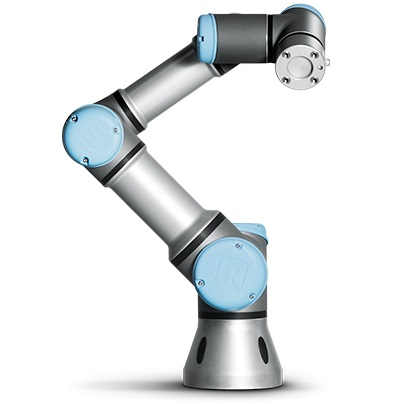
\includegraphics[scale=0.5]{image/Lab_ur3-robot-flexible-table-top-robot-big.jpg}

\vfill
\Large \textit{Liangjing Yang} \\
\Large \textit{Songjie Xiao} \\
\Large \textit{Tiexin Wang} \\
\Large \textit{Tengyue Wang}	\\
\Large \textit{Zhefan Lin}	\\
\Large \textit{Zheyuan Zhang}

\vspace{1cm}
\Large{Zhejiang University/University of Illinois at Urbana-Champaign}\\
\vspace{0.25cm}
\small{UR3e Python - ROS Interface}\\
\vspace{1cm}
\end{center}
\small{Modified from ECE470: Introduction to Robotics from University of Illinois at Urbana-Champaign
http://coecsl.ece.illinois.edu/ece470}
\end{titlepage}

%\chapter*{Acknowledgements}
%None of labs 2 through 6 would be possible without the work of Daniel Herring, the previous teaching assistant for the course who rewrote the bug-ridden Rhino interface.  I am also indebted to Robert Tao who compiled all of the lab assignments and appendices into one cohesive document and who patiently endured many formatting revisions to this manual.  I am grateful to Professor Seth Hutchinson for the privilege of working with him in 2004 and 2005 as he served as the course instructor.  It was Professor Hutchinson who suggested rewriting the lab assignments and merging them into a single lab manual.  Finally, thanks are due to the students in Introduction to Robotics who suffered through multiple drafts of each lab assignment and provided helpful feedback throughout the course.

\pagenumbering{roman}

\tableofcontents


\chapter*{Preface}
This is a set of laboratory assignments designed to complement the introductory robotics lecture taught in the College of Engineering at the University of Illinois at Urbana-Champaign.  Together, the lecture and labs introduce students to robot manipulators and computer vision along with the Robot Operating System (ROS) and serve as the foundation for more advanced courses on robot dynamics, control and computer vision.  The course is cross-listed in three departments (Electrical \& Computer Engineering, Aerospace Engineering, and Mechanical Science \& Engineering) and consequently includes students from a variety of academic backgrounds. \\

For success in the laboratory, each student should have completed a course in linear algebra and be comfortable with three-dimensional geometry.  In addition, it is imperative that all students have completed a freshman-level course in computer programming.  \textit{MODERN ROBOTICS
MECHANICS, PLANNING, AND CONTROL} (Kevin M. Lynch and Frank C. Park, 2017) is required for the lectures and will be used as a reference for many of the lab assignments.  We will hereafter refer to the textbook as \textit{MR} in this lab manual. \\

These laboratories are simultaneously challenging, stimulating, and enjoyable.  It is the author's hope that you, the reader, share a similar experience.\\

Enjoy the course! 
\thispagestyle{empty}

\mainmatter
\chapter{Introduction to the UR3}
\section{Important}
Read the entire lab before starting and especially the ``Grading" section so you know what needs to be accomplished before finishing the lab.
\section{Objectives}
The purpose of this lab is to familiarize you with the UR3 robot arm and its industrial programming interface called the teach pendant.\
In this lab, you will:
\begin{itemize}
\item Learn how to turn on and activate the UR3, and work with the teach pendant to create a simple program for the UR3
\item Use the teach pendant to turn on and off the suction cup gripper and use the gripper in a program
\item Move three stacked blocks from one position to another position using the rules specified for the Tower of Hanoi puzzle.  Blocks should be aligned on top
of each other.
\item Use high level ``\textbf{Move}" commands to move the UR3's Tool Center Point in linear and circular motions
\item Time permitting play with other functionality of the teach pendant.
\end{itemize}

\section{References}
\begin{itemize}
\item UR3 Owner's Manual:

\url{https://www.universal-robots.com/download/?option=52870#section52851}
\item UR3 Software Manual:

\url{https://www.universal-robots.com/download/?option=53077#section53064}
\item Universal Robots Academy

\url{https://www.universal-robots.com/academy/}

\item Since this is a robotics lab and not a course in computer science or discrete math, feel free to Google for solutions to the Tower of Hanoi\
problem.\footnote{\url{http://www.cut-the-knot.org/recurrence/hanoi.shtml} (an active site, as of this writing.)} You are \textbf{NOT} required to implement\
a recursive solution.
\end{itemize}

\section{Pre-Lab}
Before you come to lab it is very important that you go through the training videos found at Universal Robots website\
\url{https://www.universal-robots.com/academy/}.  These training sessions get into some areas that we will not be using in this\ 
class (for example you will not be changing safety settings), but go through all of the assignments as they will help you\ 
get familiar with the UR3 and its teach pendant.  You also may want to reference these sessions when you are in lab.

\section{Task}
The goal is to move a ``tower'' of three blocks from one of three locations on the table to another.  An example is shown in \figref{towers1}.  The\
blocks are numbered with block 1 on the top and block 3 on the bottom.  When moving the stack, two rules must be obeyed:
\begin{enumerate}
\item Blocks may touch the table in only three locations (the three ``towers'').  
\item You may not place a block on top of a lower-numbered block, as illustrated in \figref{legal1}.
\end{enumerate}

\begin{figure}
	\centering
		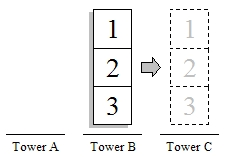
\includegraphics[scale=0.65]{image/lab1_towers.jpg}
	\caption{\figlbl{towers1} Example start and finish tower locations.}
\end{figure}

\begin{figure}
	\centering
		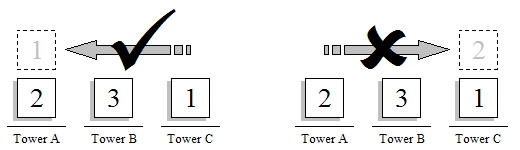
\includegraphics[scale=0.75]{image/lab1_legal.jpg}
	\caption{\figlbl{legal1} Examples of a legal and an illegal move.}
\end{figure}

\section{Procedure}
\begin{enumerate}
\item The Pre-Lab asked you to go through the basic UR3 training at Universal Robots website.  This training should have shown you how to make\ 
simple programs to move the UR3.  Initially your TA will demonstrate how to turn on and enable the UR3 as well as how to use the emergency stop\ 
button.  Then use this lab time to familiarize yourself with the UR3 robot.  First play around with simple programs that move the robot between a\ 
number of points.  
\item To turn on the suction for the suction cup gripper, \textbf{Digital output 0} needs to be set high.  Set low to turn off the suction.  Also \textbf{Digital\ 
input 0} indicates if the suction cup is gripping something.  It will return 1 if it is gripping an object and 0 if not.  Modify your above program\ 
(or make a new one) to add activating on and off the suction cup gripper.  
\item Choose the three spots on the robot's table where blocks can be placed when solving the Tower of Hanoi problem.
\item Use the provided colored tape to mark the three possible tower bases.  You should initial your markers so you can distinguish your\
tower bases from the ones used by teams in other lab sections.
\item Choose a starting position and ending position for the tower of three blocks.  Future note: In Lab 2 the user will enter the start and stop positions.

\item So you will need to use the suction cup gripper's feedback that indicates\ 
whether an object is being gripped or not.  Then with some ``\textbf{If}" instructions complete this task such that the user can put the two blocks in any of the\
three starting positions.  When you are finished, you will demo your program to your TA showning that your program works when two blocks are placed and aligned in the\
three different configurations and also does not have a problem if only one block or even no blocks are placed at their starting positions.  
Tips for creating this program:
\begin{itemize}
\item To turn on the suction cup, use the \textbf{Set} command and select \textbf{Digital Output 0} and turn it on or true.  Set it to off or false to turn off the suction.  
\item \textbf{Digital Input 0} indicates if something has been gripped by the suction cup.  Go to the \textbf{I/O} tab and turn on and off \textbf{Digital Output 0} and check which\
state of Digital Input 0 indicates gripped and upgripped.  
\item In the Structure tab under Advanced besides ``\textbf{If ... else}", you may also want to use the Assignment to create a global worker variable that, for example,\
stores the number of blocks collected.  In addition the \textbf{SubProg} item creates a subroutine that you may call when performing the same steps.  The subroutine's scope\
allows it to see the variables you create with the \textbf{Assignment} item.  
\item You may want to name your \textbf{Waypoints}.  This makes your program easier to read.  In addition if the robot needs to go to the same point multiple times\
in your program you can command it to go to the same waypoint name.  
\item Under the Structure tab you can use the \textbf{Copy} and \textbf{Paste} buttons to copy a line of code and past it in a different subsection of your code.  This cuts down\
on extra typing.  Also note the \textbf{Move} up and down buttons along with the \textbf{Cut} and \textbf{Delete} buttons.  Suppress is like commenting out a line of code.  
\item When you add an ``\textbf{If}" statement and then click on the \textbf{Command} tab, tap in the long white box to pull up the keyboard for entering the if condition.    
\end{itemize} 

\item Using the Teach Pendant create a program that solves the Tower of Hanoi problem.  Instead of using \textbf{MoveJ} moves like in Lab 1, experiment with using\
\textbf{MoveL} and \textbf{MoveP} moves.  \textbf{MoveL} moves the Tool Center Point (TCP) along a straight line, and \textbf{MoveP} is a process move that keeps the TCP moving at a constant\
speed and allows you to move along circular arcs.  Reference these three ``How To" articles from Universal Robots on creating circular arcs:
\begin {itemize}
\item \url{https://www.universal-robots.com/how-tos-and-faqs/how-to/ur-how-tos/circle-using-movec-16270/}
\item \url{https://www.universal-robots.com/how-tos-and-faqs/how-to/ur-how-tos/circular-path-using-movepmovec-15668/}
\item \url{https://www.universal-robots.com/how-tos-and-faqs/how-to/ur-how-tos/circle-with-variable-radius-15367/}
\end {itemize}
\item Demo this working program to your TA.  Your TA may ask you to improve your positioning if the stack does not end up aligned well.
Your program must have at least one obvious linear move and one obvious circular move that completely encircles one of the block positions.
\end{enumerate}
%% Updated by Ben Walt

\section{Report}
Each partner will submit a lab report using the guidelines given in the “ECE 470: How to Write a Lab Report” document.  Please be aware of the following:
\begin{itemize}
	\item Lab reports are due one week after the final session!
	\item Lab reports will be submitted online at \href{https://learn.intl.zju.edu.cn/webapps/login/}{BlackBoard}.
\end{itemize}
Your report should include the following:
\begin{itemize}
	\item Briefly explain the rules of Towers of Hanoi (Introduction/Objective)
	\item Concisely explain your solution (Method)
	\item Discuss your circular movement and how you implemented it (Method)
	\item Note anything you learned about operating the robot (Conclusion)
	\begin{itemize}
		\item How did you keep your block stacks neat?
		\item Observations about \textbf{MoveJ}, \textbf{MoveL}, and \textbf{MoveP}?
	\end{itemize}
	\item Make use of figures and tables as needed to aid in your explanation
	\item Read “ECE 470: How to Write a Lab Report” carefully so you know all the requirements
	  
\end{itemize}

\section{Demo}
Show your TA the program you created.  

\section{Grading}
\begin{itemize}
\item 10 points, completed this section by the end of the two hour lab session.  
\item 70 points, successful demonstration.
\item 20 points, report.
\end{itemize}


% \section{Preparation for Lab 2}
% In Lab 2, we will be moving on to use ROS to control the UR3.  We will use it to solve a modified version of the famous Towers of Hanoi problem.  Some suggested reading:

% \begin{itemize}
% \item Consult Appendix \ref{cprog} of this lab manual for details of ROS and Python functions used to control the UR3.
% \item ``\textit{A Gentle Introduction to ROS}", Chapter 2 and 3. \url{http://coecsl.ece.illinois.edu/ece470/agitr-letter.pdf}
% \begin{itemize}
% \item Chapter 2: 2.4 Packages, 2.5 The Master, 2.6 Nodes, 2.7.2 Messages and message types.
% \item Chapter 3 Writing ROS programs.
% \end{itemize}
% %Doesn't seem to exist anymore - Fall 2020
% %\item A short tutorial for ROS by Hyongju Park. \url{https://sites.google.com/site/ashortrostutorial/}
% \item \url{http://wiki.ros.org/}
% \item Since this is a robotics lab and not a course in computer science or discrete math, feel free to Google for solutions to\
% the Tower of Hanoi problem.\footnote{\url{http://www.cut-the-knot.org/recurrence/hanoi.shtml} (an active site, as of this writing.)} You\
% are not required to implement a recursive solution.

% \end{itemize}
\chapter{Get Started with ROS}
\section{Important}
Before this lab, please Consult \textbf{Appendix} \ref{cprog} of this lab manual for details of ROS Concepts (\textbf{Node}, \textbf{Topic}, \textbf{Message}).

\section{Objectives}
The purpose of this lab is to familiarize you with the ROS environment and its basic concepts of Node, Topic and Message through a simple turtle simulator.\
What's more, a useful tool tf is introduced, which lets user keep track of multiple coordinate frames over time.
In this lab, you will:

\begin{itemize}
	\item Learn how to show basic node, message and topic information.
	\item Learn how to publish and subscribe Messages to Topics.
	\item Learn how to transform points, vectors and other geometric entities between different coordinate frames.
\end{itemize}

\section{References}
\begin{itemize}
	\item ``\textit{A Gentle Introduction to ROS}", Chapter 2 and 3. \url{http://coecsl.ece.illinois.edu/ece470/agitr-letter.pdf}
	\begin{itemize}
		\item Chapter 2: 2.4 Packages, 2.5 The Master, 2.6 Nodes, 2.7.2 Messages and message types.
		\item Chapter 3 Writing ROS programs.
	\end{itemize}
	\item Turtlesim Documentation in ROS community.
	\url{http://wiki.ros.org/turtlesim}
\end{itemize}

\section{Procedure}

\begin{enumerate}
	\item create your own workspace according to \textbf{Appendix} \ref{cprog} of this lab manual. 
	This is the workspace you will use for the rest of the lab. DO NOT confuse it with the workspace other groups created. 
	Then copy the package \textbf{lab2pkg\_{}turtle} on your DESKTOP to your workspace \textbf{catkin\_(yourID)/src} . 
	What is IMPORTANT is to remember to source your workspace when you open a new terminal.

	\item \textbf{Starting} turtlesim: In three separate terminals, execute these three commands\\
	Hints: ctrl+alt+T(to start a new window), ctrl+shift+W(to close current window), ctrl+shift+E(split window vertically), ctrl+shift+O(split window horizontally)

\begin{lstlisting}[language=bash]
$ roscore
$ rosrun turtlesim turtlesim_node
$ rosrun turtlesim turtle_teleop_key
\end{lstlisting}

\begin{figure}
	\centering
		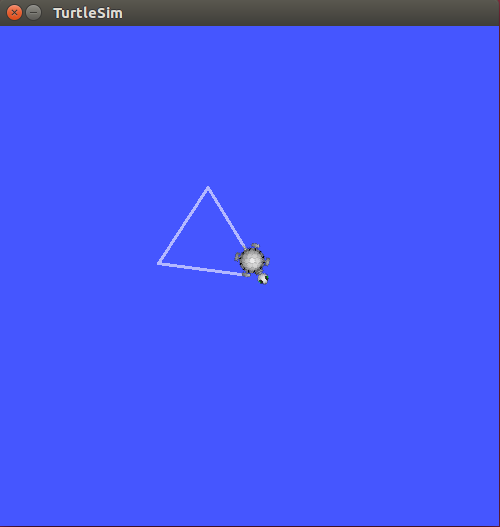
\includegraphics[scale=0.5]{image/lab2_turtlesim.png}
	\caption{\figlbl{turtle_sim} The turtlesim window}
\end{figure}

	If everything works correctly, you should see a graphical window similar to \figref{turtle_sim}.
	This window shows a simulated, turtle-shaped robot that lives in a square world.
	If you give your third terminal (the one executing the turtle\_{}teleop\_{}key command) the input focus and press the Up, Down, Left, or Right keys, the turtle will move in response to your commands, leaving a trail behind it.\\
	Making virtual turtles draw lines is not, in itself, particularly exciting.
	However, this example already has enough happening behind the scenes to illustrate many of the main ideas on which more interesting ROS systems are based.

	\item \textbf{Node} is a running instance of a ROS program. The basic command to create a node (also known as “running a ROS program”) is rosrun. ROS provides a few ways to get information about the nodes that are running
	at any particular time. To get a list of running nodes, try this command.

\begin{lstlisting}[language=bash]
# rosrun package-name executable-name
$ rosnode list
\end{lstlisting}

	If you do this in a new window, you will see a list of three nodes.

\begin{lstlisting}[language=bash]
$ /rosout
$ /turtlesim
$ /teleop_turtle
\end{lstlisting}

	The /rosout is a special node that is started automatically by roscore. Its purpose is somewhat similar to the standard output (i.e. std::cout). \\
	The other two nodes should be fairly clear: They're the simulator (turtlesim) and the teleoperation program(teleop\_{}turtle) we started ablove. \\
	You can get some information about a particular node using this command:

\begin{lstlisting}[language=bash]
$ rosnode info node-name
\end{lstlisting}

	The output includes a list of \textbf{topics} for which that node is a publisher or subscriber, the services offered by that node, its Linux process identifier
	(PID), and a summary of the connections it has made to other nodes.

	\item The primary mechanism that ROS nodes use to communicate is to send \textbf{Messages}. Messages in ROS are organized into named \textbf{Topics}.
	The idea is that a node that wants to share information will publish messages on the appropriate topic or topics;
	a node that wants to receive information will subscribe to the topic or topics that it's interested in.
	The ROS master takes care of ensuring that publishers and subscribers can find each other. \\
	This idea is probably easiest to see graphically, and the easiest way to visualize the publish-subscribe relationships between ROS nodes is to use this command:

\begin{lstlisting}[language=bash]
$ rqt_graph
\end{lstlisting}

\begin{figure}
	\centering
		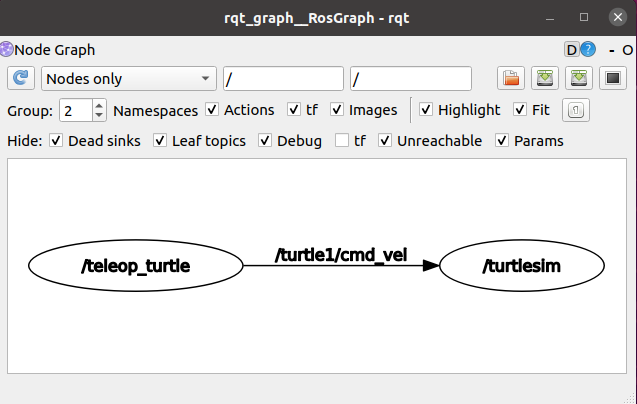
\includegraphics[scale=0.5]{image/lab2_rqt_graph.png}
	\caption{\figlbl{turtle_rqt} The rqt\_{}graph interface, showing the graph for the turtlesim example}
\end{figure}

	In this case, you will see something like \figref{turtle_rqt}. In this graph, the ovals represent nodes, and the directed edges represent publisher-subscriber relationships.
	The graph tells us that the node named /teleop\_{}turtle publishes messages on a topic called /turtle1/cmd\_{}vel, and that the node named /turtlesim subscribes to those messages. \\
	Now we can understand at least part of how the turtlesim teleoperation system works. When you press a key, the /teleop\_{}turtle node publishes messages with those movement commands on a topic called /turtle1/cmd\_{}vel. 
	Because it subscribes to that topic, the turtlesim\_{}node receives those messages, and simulates the turtle moving with the requested velocity. The important points here are:

	- The simulator doesn't care (or even know) which program publishes those cmd\_{}vel messages. Any program that publishes on that topic can control the turtle.

	- The teleoperation program doesn't care (or even know) which program subscribes to the cmd\_{}vel messages it publishes. Any program that subscribes to that topic is free to respond to those commands.
	
	\item Next let's take a closer look at the topics and messages themselves. To get a list of active topics, use this command:

\begin{lstlisting}[language=bash]
$ rostopic list
\end{lstlisting}

	In our example, this shows a list of five topics:

\begin{lstlisting}[language=bash]
$ /rosout
$ /rosout_agg
$ /turtle1/cmd_vel
$ /turtle1/color_sensor
$ /turtle1/pose
\end{lstlisting}

	You can see the autual messages that are being published on a single topic using the rostopic command, take /turtle1/pose as an exmaple:

\begin{lstlisting}[language=bash]
$ rostopic echo  /turtle1/pose
\end{lstlisting}

	your terminal will update pose data in real-time if you control the turtle by keyboard.

	Also you can learn more about a topic using the rostopic info command:

\begin{lstlisting}[language=bash]
$ rostopic info  /turtle1/pose
\end{lstlisting}

	You should see output similar to this:

\begin{lstlisting}[language=bash]
Type: turtlesim/Pose

Publishers:
  * /turtlesim (http://rvc-ece470:43601/)

Subscribers: None

\end{lstlisting}

	The most important part of this output is the very first line, which shows the \textbf{message type} of that topic. In the case of \textbf{/turtle1/pose}, the message type is 
	\textbf{turtlesim/Pose}. The message type of a topic tells you what information is included in each message on that topic, and how that information is organized.

	To see details about a message type, use a command like this:

\begin{lstlisting}[language=bash]
$ rosmsg show message-type-name
\end{lstlisting}

	Let's try using it on the message type for /turtle1/pose that we found above:

\begin{lstlisting}[language=bash]
$ rosmsg show turtlesim/Pose
\end{lstlisting}
	
	The output is:

\begin{lstlisting}[language=bash]
float32 x
float32 y
float32 theta
float32 linear_velocity
float32 angular_velocity
\end{lstlisting}

	The format is a list of fields, one per line. Each field is defined by a built-in data type (like int8, bool, or string) and a field name.
	The output above tells us that a turtlesim/Pose is a thing that contains five float32 items.

	Another example, one we'll revisit several times, is geometry\_{}msgs/Twist. This is the message type for the /turtle1/cmd\_{}vel topic, and it is slightly more complicated:

\begin{lstlisting}[language=bash]
geometry_msgs/Vector3 linear
	float64 x
	float64 y
	float64 z
geometry_msgs/Vector3 angular
	float64 x
	float64 y
	float64 z
\end{lstlisting}

	In this case, both linear and angular are \textbf{composite fields} whose date type is geometry\_{}msgs/Vector3. The indentation shows that fields named x, y, and z aremembers within
	those two top-level fields. That is, a message with type geometry\_{}msgs/Twist contains exactly six numbers, organized into two vectors called linear and angular. Each of these
	numbers has the built-in type float64.

	\item Finally, let's try to publish velocity command to the turtle in command line instead of using keyboard.
	We will use \textbf{rostopic pub} command to publish a message to a topic.

\begin{lstlisting}[language=bash]
$ rostopic pub /turtle1/cmd_vel geometry_msgs/Twist
$ "linear:
$   x: 1.0
$   y: 0.0
$   z: 0.0
$ angular:
$   x: 0.0
$   y: 0.0
$   z: -1.0" -r 1
\end{lstlisting}

	Here we are publishing a message of type geometry\_{}msgs/Twist to the topic /turtle1/cmd\_{}vel. The message is specified on the command line, and the -r option tells rostopic pub to
	publish the message repeatedly at a rate of 1 Hz. The message is specified in YAML format, which is a simple text-based format for representing structured data. The message we are
	sending is a Twist message with linear velocity 1.0 in the x direction and angular velocity -1.0 in the z direction. The turtle should move in a circle.\\
	Hint: you can utilize the full convenience of the command line by using the \textbf{tab} key to autocomplete the topic name and message type.\\

\end{enumerate}

\section{Task}

In order to master above concepts, here is one simple practice for you. We will have two turtles, as is shown in \figref{turtle_chase}. One is leader and the other is follower.
The leader turtle is controlled by keyboard input and the follower turtle should be programed to follow the trajectory.
what you should do is to write a program to make the follower turtle follow the leader turtle.\\

\begin{figure}
	\centering
		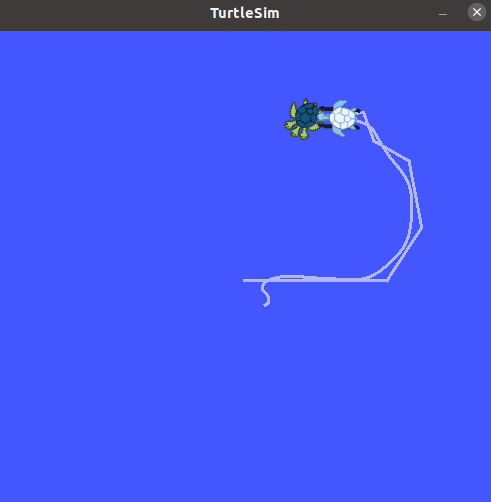
\includegraphics[scale=1]{image/lab2_turtle_chase.png}
	\caption{\figlbl{turtle_chase} turtle chase and catch game }
\end{figure}

Here give a brief introduction of the package \textbf{tf} we will use in this lab.
The \textbf{tf} package is used to keep track of multiple coordinate frames over time.

\begin{lstlisting}[language=bash]
$ roslaunch lab2pkg_turtle turtle_tf2_demo.launch
\end{lstlisting}

You will see the turtlesim start with two turtles. Once the turtlesim is started you can drive the central turtle around in the turtlesim using the keyboard arrow keys, 
select the second terminal window so that your keystrokes will be captured to drive the turtle.

This demo is using the tf2 library to create three coordinate frames: a \textbf{world} frame, a \textbf{turtle1} frame, and a \textbf{turtle2} frame.
This demo uses a tf2 broadcaster to publish the turtle coordinate frames.

\textbf{tf\_echo} reports the transform between any two frames broadcasted over ROS.

\begin{lstlisting}[language=bash]
$ rosrun tf tf_echo /world /turtle1
\end{lstlisting}

You will see the transform displayed as the \textbf{tf2\_echo} listener receives the frames broadcasted over ROS.

\begin{lstlisting}[language=bash]
At time 1622031731.625364060
- Translation: [2.796, 1.039, 0.000]
- Rotation: in Quaternion [0.000, 0.000, 0.202, 0.979]
At time 1622031732.614745114
- Translation: [1.608, 0.250, 0.000]
- Rotation: in Quaternion [0.000, 0.000, 0.032, 0.999]
\end{lstlisting}

As you drive your turtle around you will see the transform change as the two turtles move relative to each other.

Also \textbf{rviz} is a visualization tool that is useful for examining tf2 frames. 
Let's look at our turtle frames using rviz. Let's start rviz with the turtle\_rviz.rviz configuration file using the \textbf{-d} option:

\begin{lstlisting}[language=bash]
$ rosrun rviz rviz -d ${rospack find lab2pkg_turtle}/config/turtle_rviz.rviz
$ or
$ rosrun rviz rviz -d {your absolute path to turtle_rviz.rviz}
\end{lstlisting}

In the side bar you will see the frames broadcasted by tf2. As you drive the turtle around you will see the frames move in rviz.

Now you can start to write your own program to make the follower turtle follow the leader turtle.\\

\begin{figure}
	\centering
		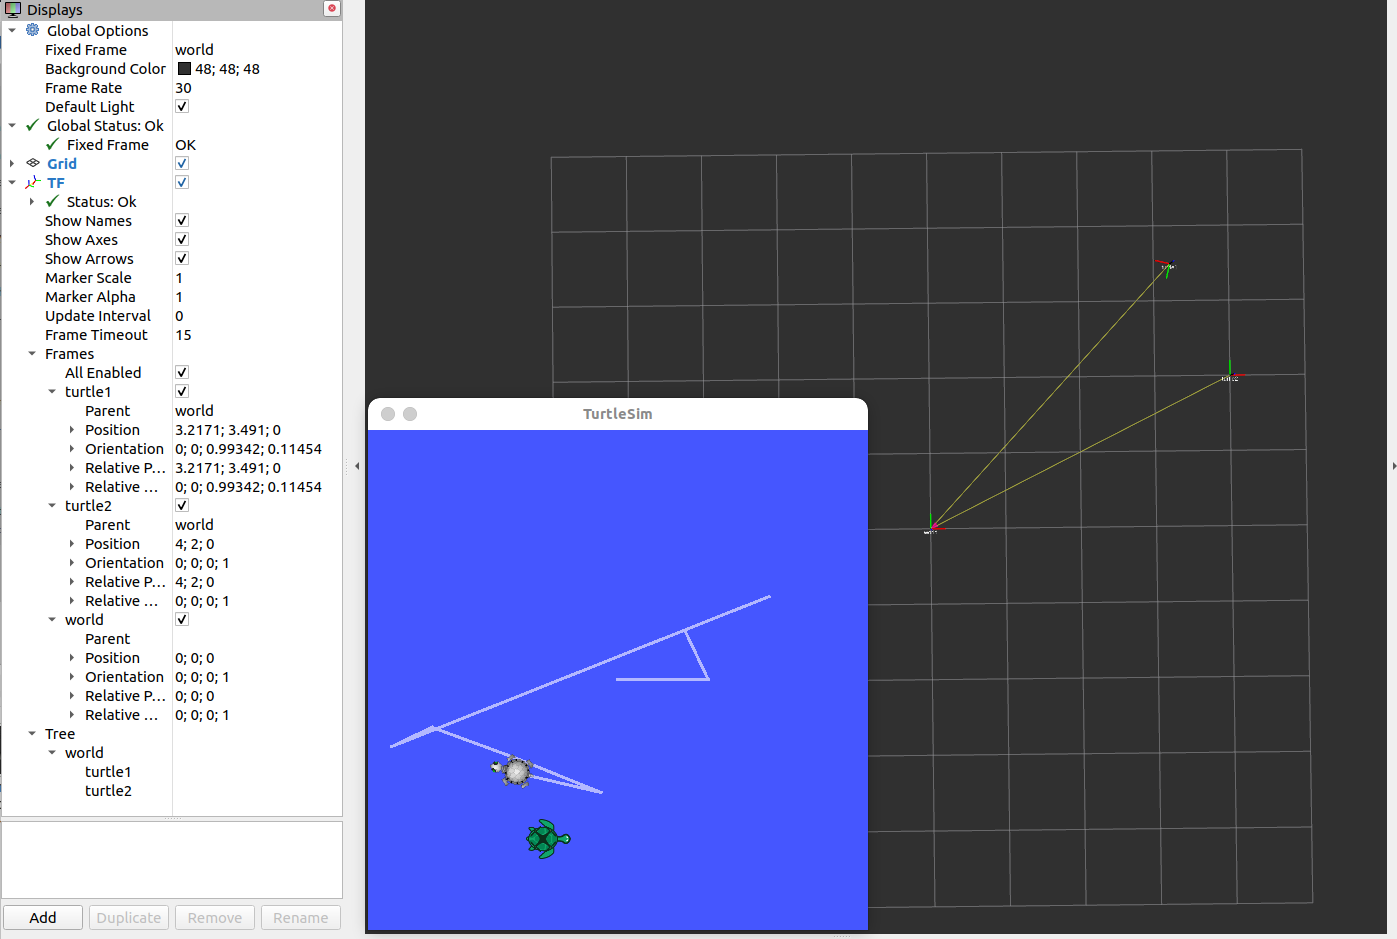
\includegraphics[scale=0.25]{image/lab2_turtle_rviz.png}
	\caption{\figlbl{turtle_rviz} The turtlesim window}
\end{figure}

\begin{enumerate}
	\item Establish your own workspace as shown in Appendix \ref{cprog} and all your programming work will be done here.
	\item Copy package \textbf{lab2pkg\_{}turtle} into your workspace. All your source code is in folder \textbf{ECE470\_LAB} on your desktop. Do Not Modify it!
	\item Complete your code and see how to run it in \textbf{README.md}.
\end{enumerate}

\section{Report}

Each partner will submit a lab report using the guidelines given in the “ECE 470: How to Write a Lab Report” document.  Please be aware of the following:
\begin{itemize}
	\item Lab reports are due one week after the final session!
	\item Lab reports will be submitted online at \href{https://learn.intl.zju.edu.cn/webapps/login/}{BlackBoard}.
\end{itemize}

\section{Demo}
Show your TA the program you created.  

\section{Grading}
\begin{itemize}
\item 10 points, completed this section by the end of the two hour lab session.  
\item 70 points, successful demonstration.
\item 20 points, report.
\end{itemize}



\chapter{The Tower of Hanoi with ROS}
\section{Important}
Read the entire lab before starting and especially the ``Grading" section so you are aware of all due dates and requirements associated with the lab.  Hopefully you are reading this well before your lab section meets as given the compressed schedule, it is very important that you arrive at lab well prepared.  This semester, the more you do prior to your lab session, the more you will get out of the short time you have with the TA.
% \todo[inline]{Need to change these}
\section{Objectives}
This lab is an introduction to controlling the UR3e robot using the Robot Operating System (ROS) and the Python programming language.  In this lab, you will:
\begin{itemize}
% \item Record joint angles that position the robot arm at waypoints in the Tower of Hanoi solution
\item Modify the given starter python file to move the robot to waypoints and enable and disable the suction cup gripper such that the blocks are moved in the\
correct pattern.
\item If the robot suction senses that a block is not in the gripper when it should be, the program should halt with an error.
\item Program the robot to solve the Tower of Hanoi problem allowing the user to select any of three starting positions and ending positions.
\end{itemize}

\newpage
\section{Pre-Lab}
Read ``\textit{A Gentle Introduction to ROS}", available online, Specifically:
\begin{itemize}
\item Chapter 2: 2.4 Packages, 2.5 The Master, 2.6 Nodes, 2.7.2 Messages and message types.
\item Chapter 3 Writing ROS programs.
\end{itemize}
\section{References}
\begin{itemize}
\item Consult Appendix \ref{cprog} of this lab manual for details of ROS and Python functions used to control the UR3e.
\item ``\textit{A Gentle Introduction to ROS}", Chapter 2 and 3. \url{http://coecsl.ece.illinois.edu/ece470/agitr-letter.pdf}
% I can't find this anymore Fall 2020
% \item A short tutorial for ROS by Hyongju Park. \url{https://sites.google.com/site/ashortrostutorial/}
\item \url{http://wiki.ros.org/}
\item Since this is a robotics lab and not a course in computer science or discrete math, feel free to Google for solutions to\
the Tower of Hanoi problem.\footnote{\url{http://www.cut-the-knot.org/recurrence/hanoi.shtml} (an active site, as of this writing.)} You\
are not required to implement a recursive solution.

\end{itemize}

\newpage
\section{Task}
% \todo[inline]{I think we should describe traditional TOH and then explain how ours works.  We also will want figures.}
\subsection{Standard Tower Of Hanoi}
As you hopefully know by now, the normal way that the Tower of Hanoi puzzle is set up is as a stack of discs or blocks as seen in \figref{towers}.  This makes many of the rules obvious such as that you cannot move a lower block while a higher block still rests on it.  This arrangement is hard to simulate in Gazebo (The simulator we will be using).  Stacked blocks do not behave in a stable manner and thus it is difficult to create neat stacks without disturbing/toppling them.  As an alternative, we have modified the puzzle to work with the simulator.

\subsection{Simulated Tower Of Hanoi}
In our version of Tower of Hanoi, we have laid the blocks flat on the table as seen in \figref{towers2d}.  Now, instead of rising vertically from the table, the blocks ``rise" as they move farther from the viewer.  Thus the ``towers" form the columns of a grid, while the ``height" depends on the rows of the grid.  We will make use of this matrix like structure to organize our waypoints in the code.
% The original goal of Tower of Hanoi is to move a ``tower'' of three blocks from one of three locations on the table to another. Due to the limitations of simulator, the tower is "2D" (lying on the table) instead of 3D one which you stack vertically. So instead of stacking the blocks upwards, you are "stacking" the blocks towards the robot base horizontally. 

% An example is shown in \figref{towers}.  The blocks are numbered with block 1 on the top and block 3 on the bottom. The blocks are color-coded in the simulator, and it corresponds to the numbers in the following order:

Color has been used to help keep track of the blocks in the simulator:
\begin{enumerate}
    \item Red - Top Block
    \item Yellow - Middle Block
    \item Green - Bottom Block
\end{enumerate}

This "2D" version doesn't have gravity to enforce building from "bottom" to "top", but you should still code it as if it has gravity (i.e. no floating blocks). You may not place a block on top of a lower-numbered block, as illustrated in \figref{illegal}. (For example, no green block on top of red or yellow blocks.)  An example of a legal move can be seen in \figref{legal}.

In addition, unlike an actual vacuum gripper, the vacuum gripper in the simulator has to go to the center of an object in order to actually grip it. Due to this difference, you will be given two files that record the locations of towers corresponding to the actual lab environment and the simulator environment.

For this lab, we will complicate the task slightly.  Instead of a set start and end position, your python program should use the robot to move a tower from {\it any} of the three\
locations to {\it any} of the other two locations.  Therefore, you should prompt the user to specify the start and destination locations for the tower.

Additionally, you will make use of suction feedback to verify that you have grasped the desired block successfully.  If a block is missing, the robot should stop the puzzle, shut off the gripper and return to its home position.

\begin{figure}
	\centering
		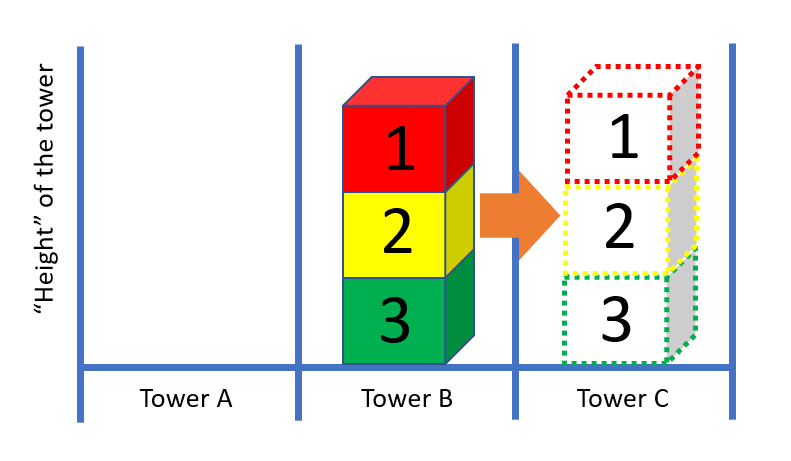
\includegraphics[scale=0.5]{image/lab3_3d_goal.png}
	\caption{\figlbl{towers} Standard Tower of Hanoi configuration with blocks stacked on top of each other.}
\end{figure}

\begin{figure}
	\centering
		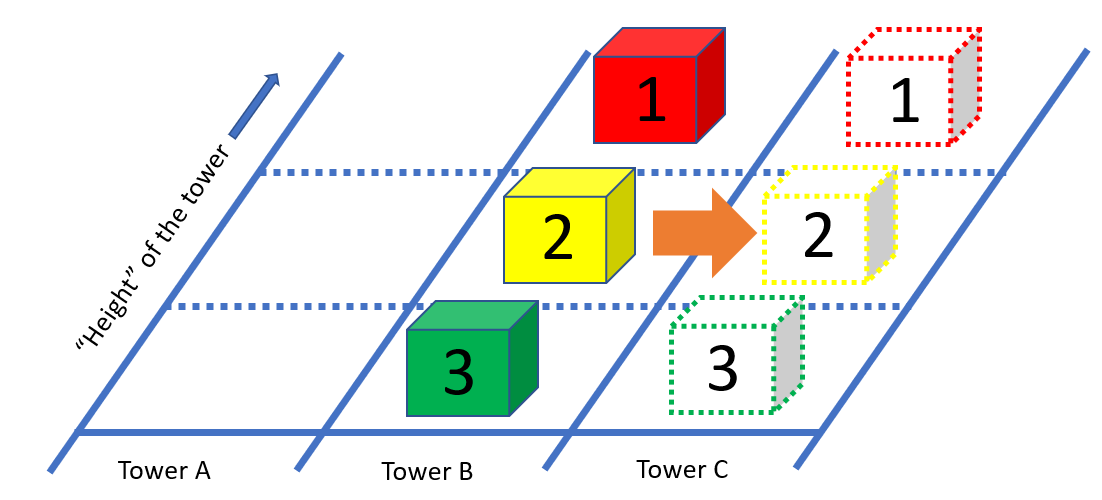
\includegraphics[scale=0.4]{image/lab3_2d_goal.png}
	\caption{\figlbl{towers2d} Example start and finish tower locations in the simulated version of the puzzle.}
\end{figure}

\begin{figure}
	\centering
		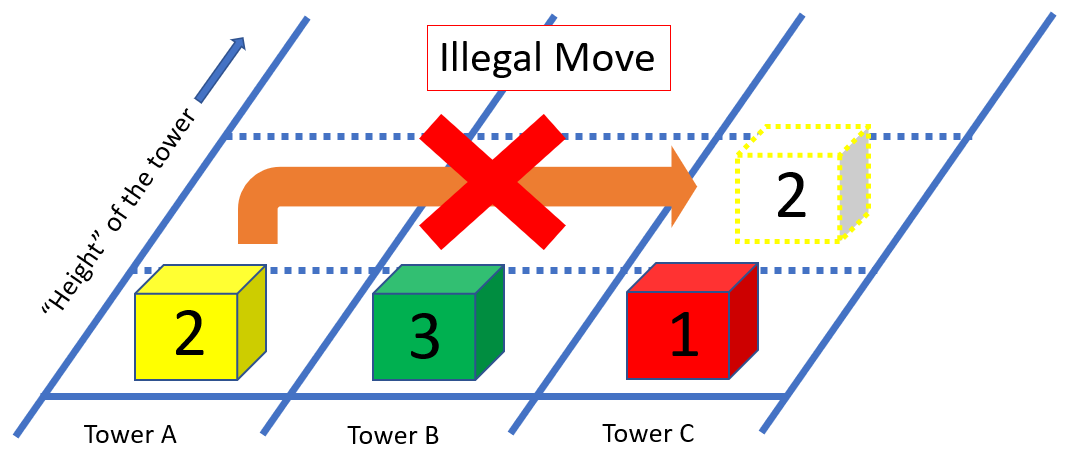
\includegraphics[scale=0.4]{image/lab3_2d_illegal.png}
	\caption{\figlbl{illegal} Example of an illegal move.}
\end{figure}

\begin{figure}
	\centering
		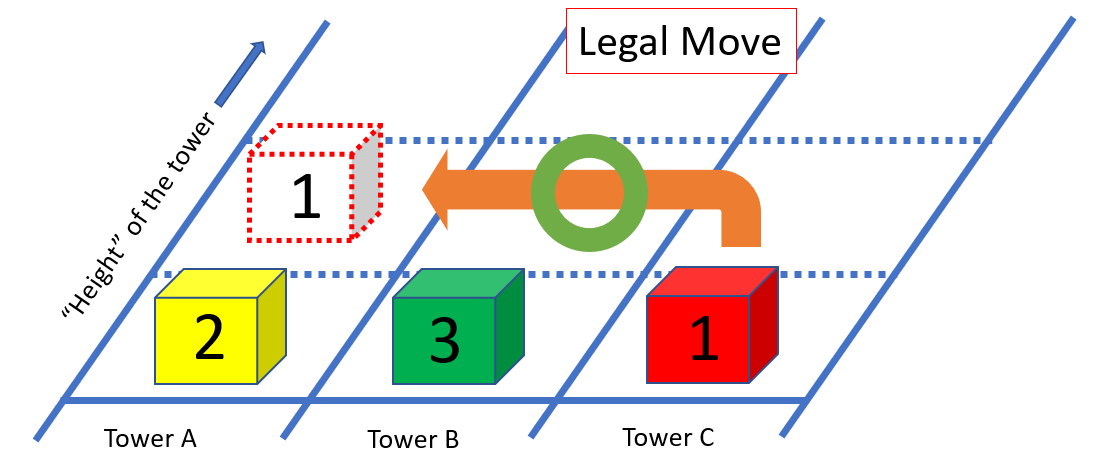
\includegraphics[scale=.4]{image/lab3_2d_legal.png}
	\caption{\figlbl{legal} Example of a legal move.}
\end{figure}



\newpage
\section{Procedure}
\begin{enumerate}
\item Create your own workspace as shown in Appendix \ref{cprog}.
\item Copy package \textbf{lab3pkg\_hanoi} into your workspace from \textbf{ECE470\_LAB}. All your coding work will be done in the script \textbf{lab3\_exec.py} with comments. Refer to \textbf{README.md} on how to run your code and robot!

\begin{itemize}
\item \textbf{lab3\_exec.py} a file in scripts folder with skeleton code to get you started on this lab. See Appendix \ref{cprog} for how to use basic ROS. Students are encouraged to make their own "cheat sheet" for some commonly used ROS and Linux commands. Also\
read carefully through the below section that takes you line by line through the starter code.  
\item \textbf{CMakeLists.txt} a file that sets up the necessary libraries and environment for compiling lab3\_exec.py.
\item \textbf{package.xml} This file defines properties about the package including package dependencies.
\item \textbf{README} To run lab3 code on real robot, please read it \textbf{FIRST}!
\item Every time you open a new terminal, make sure to source your workspace by running \textbf{source devel/setup.bash} in your workspace folder.
\end{itemize}

\item Modify \textbf{lab3\_exec.py} to prompt the user for the start and destination tower locations (you may assume that the user will not\
choose the same location twice) and move the blocks accordingly using the suction cup to grip the blocks.  The starter file performs basic motions 
but provides a function definition for moving blocks (\textbf{move\_block}). Once you understand
the starter code moving from one position to the next, clean up the code by completing the shell function \textbf{move\_block}.  
\textbf{move\_block} picks up a block from a tower and places it on another tower. You may also create other functions for prompting user input and solving the Tower of Hanoi problem given starting and ending locations but these are not required.  
\item Add one more feature to your program.  As you saw in Lab 1.5, the Coval device that is creating the vacuum for the gripper also senses
the level of suction being produced indicating if an item is in the gripper.  Recall that \textbf{Digital Input 0} are connected to
this feedback.  Use \textbf{Digital Input 0} to determine if a block is held by the gripper.  If no block is found where a block should be,
have your program exit, turn off the gripper, return home and print an error to the console.\\
To figure out how to do this with ROS you are going to have to do a bit of ``ROS" investigation.  Use ``\textbf{rostopic list}", ``\textbf{rostopic info}" and ``\textbf{rosmsg list}" to discover
what topic to subscribe and what message will be recieved in your subscribe callback function.  Once you find the topic and message run ``\textbf{rosmsg info}"
to figure out what variable you will need to read from the message sent to your callback function.  Just like the global variables thetas that
save the positions of the robot joints inside the call back \textbf{position\_callback()}, create global variables
to communicate to your code the state of \textbf{Digital Input 0}.  Normally once you figure out which message you will be using 
you need to import it in the \textbf{lab3\_header} file that defines this message.  The \textbf{lab3\_header} file has already imported it in \textbf{lab3\_header.py} for you.  Use the explanation below
and the given code in \textbf{lab3\_exec.py} that creates the subscription to \textbf{/joint\_states} and its callback function as a guide to subscribe to the rostopic
that publishes the IO status.     

\end{enumerate}

\section{Lab3\_exec.py Explained}
First open up \textbf{lab3\_exec.py} and read through the code and its comments as this is the latest version of Lab 2's starter code. Below is the same \textbf{lab3\_exec.py}\
file listing with code comments removed and possible small differences due to changes in the lab.  If you find a difference go with the actual \textbf{lab3\_exec.py}\
file as the correct version.  \textbf{lab3\_exec.py} is broken down into sections and described in more detail below.  

{\footnotesize
%\tiny{
%\begin{verbatim}[obeytabs,tabsize=4]
%\footnotesize{
\begin{verbatim}
import copy
import time
import rospy
import numpy as np
from lab3_header import *

# 20Hz
SPIN_RATE = 20 
    
# UR3 home location
home = np.radians([-87.42, -103.45, -72.77, -79.02, 89.95, 129.93])
    
# UR3 current position, using home position for initialization
current_position = copy.deepcopy(home)
    
thetas = [0.0, 0.0, 0.0, 0.0, 0.0, 0.0]
    
digital_in_0 = 0
analog_in_0 = 0
    
suction_on = True
suction_off = False
    
current_io_0 = False
current_position_set = False

Q = None
\end{verbatim}}

You can find \textbf{lab3\_header.py} in the \textbf{lab3pkg\_py/scripts} directory.  It includes all needed files to allow \textbf{lab3\_exec.py} to call ROS functionality.
\textbf{SPIN\_RATE} will be used as the publish rate to send commands to the ROS driver. This block also initializes positions such as the home position and a global variable to store the current position. There are also some other global variables for storing the input/feedback states and also some constants. You should use these global variables and constants in different functions to help you finish the task.

Q is a list that stores all the necessary waypoints for the robot to pick and place the blocks in order to solve the Tower of Hanoi. In each entry of Q[tower index][block height][above block/on block], there are six angles in radians that correspond to the arm's six joint angles. Q is defined as illustrated below:

\begin{figure}[h]
    \centering
    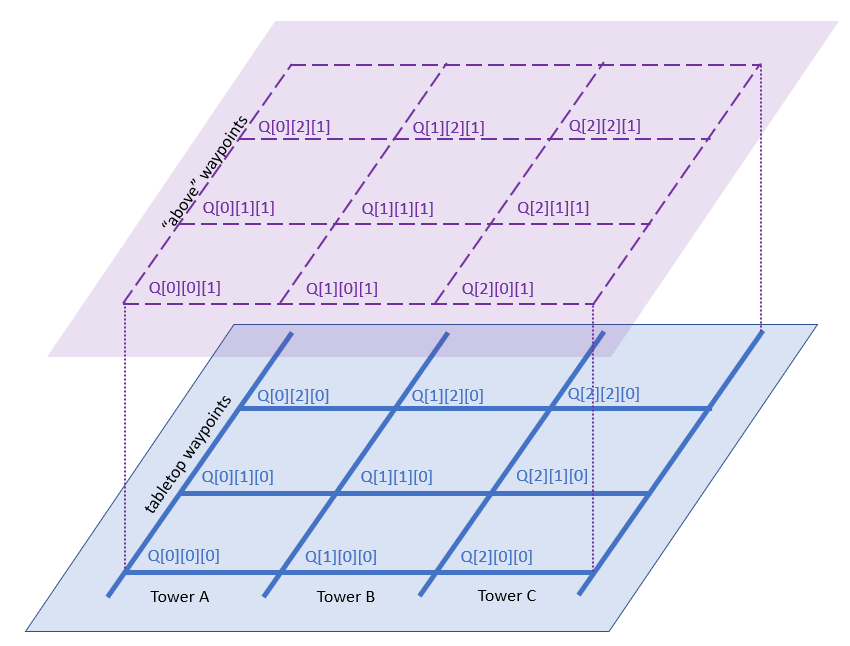
\includegraphics[scale=0.5]{image/lab3_waypoints.png}
    \caption{Waypoints Matrix Q}
\end{figure}
 
{\footnotesize
\begin{verbatim}
def position_callback(msg):

    global thetas
    global current_position
    global current_position_set

    thetas[0] = msg.position[0]
    thetas[1] = msg.position[1]
    thetas[2] = msg.position[2]
    thetas[3] = msg.position[3]
    thetas[4] = msg.position[4]
    thetas[5] = msg.position[5]

    current_position[0] = thetas[0]
    current_position[1] = thetas[1]
    current_position[2] = thetas[2]
    current_position[3] = thetas[3]
    current_position[4] = thetas[4]
    current_position[5] = thetas[5]

    current_position_set = True
\end{verbatim}}

This is \textbf{lab3\_node}'s callback function that is called when the \textbf{ur\_hardware\_interface} publishes new position data.  \textbf{ur\_hardware\_interface} publishes new
angle position data every 8ms, so this function \textbf{position\_callback} is run every 8ms.  
   
Next in \textbf{lab3\_exec.py} are the function \textbf{gripper()} and \textbf{move\_arm()}.  These functions are passed variables that are initialized at the beginning of the file. The program runs from the main function, so it will
be explained first and then we will come back to \textbf{gripper()} and \textbf{move\_arm()}.
   
{\footnotesize
\begin{verbatim}
def main():
    global home
    global Q
    global SPIN_RATE

    # Initialize ROS node
    rospy.init_node('lab3_node')

    # Initialize publisher for ur3e_driver_ece470/setjoint with buffer size of 10
    pub_setjoint = rospy.Publisher('ur3e_driver_ece470/setjoint',JointTrajectory,queue_size=10)
    
    # Initialize subscriber to /joint_states and callback fuction
    sub_position = rospy.Subscriber('/joint_states', JointState, position_callback)
\end{verbatim}}

To start as a ROS node the \textbf{rospy.init\_node()} function needs to be called.  Then the node needs to setup which other nodes it receives data from and which nodes\
it sends data to.  This code first specifies that it will be publishing a message to the ``\textbf{ur3e\_driver\_ece470}" node ``\textbf{setjoint}" subscriber.\
The message it will be sending is the \textbf{command} message which consists of\
the desired robot joint angles, the velocity of each joint and the acceleration of each joints.  Next \textbf{lab3\_node} subscribes to\
``\textbf{ur\_hardware\_interface}" node ``\textbf{joint\_states}" publisher.  Whenever new joint angles are\
ready to be sent, the callback function ``\textbf{position\_callback}" is called and passed the message \textbf{position} which\
contains the six joint angles.
As an exercise in lab, see if you can list the ``\textbf{ur3e\_driver\_ece470}", ``\textbf{ur\_hardware\_interface}" node and\
``\textbf{ur3e\_driver\_ece470/setjoint}" subscriber and ``\textbf{joint\_states}" publisher using the ``\textbf{rostopic list}" command in your \textbf{catkin\_ work directory}.  Also use ``\textbf{rostopic info}" to double\
check that ``\textbf{ur3e\_driver\_ece470/setjoint}" is a subscriber and ``\textbf{joint\_states}" is a publisher.  Also run ``\textbf{rosmsg list}" to find the messages.  

{\footnotesize
\begin{verbatim}   
    input_done = 0
    loop_count = 0
    
    while(not input_done):
        input_string = raw_input("Enter number of loops <Either 1 2 3 or 0 to quit> ")
        print("You entered " + input_string + "\n")
    
        if(int(input_string) == 1):
            input_done = 1
            loop_count = 1
        elif (int(input_string) == 2):
            input_done = 1
            loop_count = 2
        elif (int(input_string) == 3):
            input_done = 1
            loop_count = 3
        elif (int(input_string) == 0):
            print("Quitting... ")
            sys.exit()
        else:
            print("Please just enter the character 1 2 3 or 0 to quit \n\n")
	
\end{verbatim}}

This standard python code printing messages to the command prompt and receiving text input from the command prompt.  It loops until the correct data is input. 

{\footnotesize
\begin{verbatim}
    # Check if ROS is ready for operation
    while(rospy.is_shutdown()):
        print("ROS is shutdown!")

    rospy.loginfo("Sending Goals ...")
	
    loop_rate = rospy.Rate(SPIN_RATE)
\end{verbatim}}

Here the code waits for \textbf{roscore} to be executed and ready.  \textbf{rospy.loginfo} prints a message to the command prompt.  \textbf{rospy.Rate(SPIN\_RATE)} sets up a\
class \textbf{loop\_rate} that can be used to sleep the calling process.  The amount of time that the process will sleep is determined by the \textbf{SPIN\_RATE} parameter.\
In our case this is set to 20Hz or 50ms.  \textbf{loop\_rate} does not wake up 50 ms after it has been called, instead it wakes up the process every 50ms.  \textbf{loop\_rate}\
keeps track of the last time it was called to determine how long to sleep the process to keep a consistent rate.    
   
{\footnotesize
\begin{verbatim}
    move_block(pub_setjoint, pub_setio, start, 0, des, 2)

\end{verbatim}}

This moves the arm to a number of positions to give you a start at how to program the robot to move to different positions.  See the move\_arm
and gripper function definitions below.

{\footnotesize
\begin{verbatim}

    def move_arm(pub_setjoint, dest):
    msg = JointTrajectory()
    msg.joint_names = ["shoulder_pan_joint", "shoulder_lift_joint", 
       "elbow_joint","wrist_1_joint", "wrist_2_joint", "wrist_3_joint"]
    point = JointTrajectoryPoint()
    point.positions = dest
    point.time_from_start = rospy.Duration(2)
    msg.points.append(point)
    pub_setjoint.publish(msg)
    time.sleep(2.5)    

\end{verbatim}}

The \textbf{move\_arm()} function takes as parameters \textbf{pub\_setjoint}, which is the publisher to \textbf{ur3e\_driver\_ece470} commanding a new position for the robot to move
to. \textbf{dest} is the six joint angle destinations, in radians, that the robot will be commanded to move to.  
The code creates a variable \textbf{msg} which is the command message to be sent \textbf{ur3e\_driver\_ece470}.  \textbf{msg} is assigned the \textbf{joint\_names}, \textbf{positions} and \textbf{time\_from\_start}.
Next the \textbf{msg} is published to \textbf{ur3e\_driver\_ece470} with the \textbf{pub\_setjoint.publish(msg)} instruction.
\textbf{time.sleep(2.5)} will sleep 2.5s waiting for the robot getting to the commanded position.


% {\footnotesize
% \begin{verbatim}
% def gripper(pub_cmd, loop_rate, io_0):

%     global SPIN_RATE
%     global thetas
%     global current_io_0
%     global current_position

%     error = 0
%     spin_count = 0
%     at_goal = 0

%     current_io_0 = io_0

%     driver_msg = command()
%     driver_msg.destination = current_position
%     driver_msg.v = 1.0
%     driver_msg.a = 1.0
%     driver_msg.io_0 = io_0   
%     pub_cmd.publish(driver_msg)

%     while(at_goal == 0):

%         if( abs(thetas[0]-driver_msg.destination[0]) < 0.0005 and \
%             abs(thetas[1]-driver_msg.destination[1]) < 0.0005 and \
%             abs(thetas[2]-driver_msg.destination[2]) < 0.0005 and \
%             abs(thetas[3]-driver_msg.destination[3]) < 0.0005 and \
%             abs(thetas[4]-driver_msg.destination[4]) < 0.0005 and \
%             abs(thetas[5]-driver_msg.destination[5]) < 0.0005 ):

%             at_goal = 1
		
%         loop_rate.sleep()

%         if(spin_count >  SPIN_RATE*5):
%             pub_cmd.publish(driver_msg)
%             rospy.loginfo("Just published again driver_msg")
%             spin_count = 0

%         spin_count = spin_count + 1

%     return error
% \end{verbatim}}

% The \textbf{gripper()} function is very similar to the \textbf{move\_arm()} function above.  The same \textbf{pub\_cmd} and \textbf{loop-rate} are passed to \textbf{gripper()} but only the On/Off
% desired state of the suction cup gripper is the remaining parameter.  Looking at the \textbf{move\_arm()} function \textbf{gripper()} looks very similar but the
% robot joint destination is the current state of the arm so the robot is already at that position so it does not move.  All that the command
% changes is whether the suction gripper is On or Off by setting \textbf{driver\_msg.io\_0} equal to the passed parameter \textbf{bool io\_0}.  See the \textbf{move\_arm()}
% description for more details on this code.    


{\footnotesize
\begin{verbatim}
def move_block(pub_setjoint, pub_setio, start_loc, start_height, end_loc, end_height):
    global Q
\end{verbatim}}

The \textbf{move\_block()} function definition is provided and should be used to complete the assignment. Functions are useful when the same procedure is used many
times.  To move a block, multiple arm movements are necessary along with gripper
actuation. Instead of cluttering the main with many calls to \textbf{move\_arm} and \textbf{gripper()}, you will compartmentalize the calls in the \textbf{move\_block} function.
Use this function to compartmentalize moving a block from one tower to another. 
The start and end locations are integers given to tower positions and the heights are integers for blocks in the stack.


% \todo[inline]{A lot of this might change}

\section{Report}
Each student will submit a lab report using the guidelines given in the “ECE 470: How to Write a Lab Report” document.  Please be aware of the following:
\begin{itemize}
    \item Lab reports will be submitted online at \href{https://learn.intl.zju.edu.cn/webapps/login/}{BlackBoard}.
    \item The report will be due \textbf{Two} weeks after your lab session for Lab 2.  Exact times and dates can be seen on \href{https://learn.intl.zju.edu.cn/webapps/login/}{BlackBoard}.

\end{itemize}
Your report should include the following:
\begin{itemize}	
	\item Briefly explain the objective of the lab i.e. the goal and rules of Tower of Hanoi.  Images would greatly aid in this explanation.
	\item What was the focus of this lab? (Hint: ROS and implementing feedback)
	\item With that in mind you should cover the following (in detail):
	\begin{itemize}
		\item What is ROS and how does it work? (What kind of figure would help explain this?)
		\item How did you use the ROS commands (i.e. \textbf{rostopic list}, \textbf{rostopic info}, etc.) to complete your task?
		\item How did you implement feedback?
	\end{itemize}
	\item Make use of code snippets as needed to aid in your explanation
	\item \textbf{Read “ECE 470: How to Write a Lab Report” carefully so you know all the requirements.}
	\item Unless your TA gives other guidance, include your \textbf{lab3\_exec.py} code as an Appendix to your report	as described in lab report guidelines.
\end{itemize}

% \todo[inline]{Does this make sense schedule wise?  1 week after lab, they will be in their off week.  Are in-person demos optional?  I am not sure that I like just 1 week for demo, that is stricter than normal lab.}
\section{Demo}
% Demonstrations of your working code will either be done in-person or over Zoom.  They will be done live (i.e. no recordings) with your lab section TA.  Demos are due \textbf{2} weeks after your lab session.

% The default method of demonstrating your work will be via the simulation.  While we want to encourage in-person students to run their code on the real robot, due to time limitations, this may be difficult to do with your TA by the due date.  You can always run it for your own satisfaction at another time.
% \subsection{Demo Process}
Your TA will require you to run your program (at least) twice; on each run, the TA will specify a different set of start and destination locations for the tower.  They will also test that suction feedback has been implemented correctly.


\section{Grading}
\begin{itemize}
\item 80 points, successful demonstration.
\item 20 points, report.
\end{itemize}

% \setcounter{chapter}{2}
\chapter{Forward Kinematics}
\section{Important}
Read the entire lab before starting and especially the ``Grading" section so you are aware of all due dates and requirements associated with the lab.  Hopefully you are reading this well before your lab section meets as given the compressed schedule, it is very important that you arrive at lab well prepared.  This semester, the more you do prior to your lab session, the more you will get out of the short time you have with the TA.
\section{Objectives}
The purpose of this lab is to implement the exponential forward kinematics on the UR3e robot to estimate the end-effector pose given a set of joint angles.  In this lab you will:
\begin{itemize}
	\item Solve the exponential forward kinematic equations for the UR3e.
	\item Write a Python function that moves the UR3e to a configuration specified by the user.
	\item Compare your exponential forward kinematic estimation with the actual robot movement. 
\end{itemize}

\section{References}
\begin{itemize}
\item Chapter 4 of \textit{Modern Robotics} provides details of how to construct an exponential forward kinematic for an open-chain robot.
\end{itemize}

\section{Tasks}

\subsection{Theoretical Solution}
Find the forward kinematic equations for the UR3e robot using the exponential forward kinematics method.  Solve for $T_{06}$ and record the 6 matrices defined by $e^{[S_1]\theta_1}$ through $e^{[S_6]\theta_6}$.

\subsection{Physical Implementation} \label{sec:physical}
The user will provide six joint angles $\left\{\theta_1,\theta_2,\theta_3,\theta_4,\theta_5,\theta_6\right\}$, all given in degrees.  The angle ranges are as follows:

\begin{eqnarray*}
-90^{\circ}<&\theta_1&<90^{\circ}\\
-180^{\circ}<&\theta_2&<0^{\circ}\\
-5^{\circ}<&\theta_3&<140^{\circ}\\
-95^{\circ}<&\theta_4&<-5^{\circ}\\
-115^{\circ}<&\theta_5&<70^{\circ}\\
-170^{\circ}<&\theta_6&<170^{\circ}
\end{eqnarray*}

Note that these ranges are approximate and vary slightly from machine to machine.  If you receive a protective stop, note the affected joint on the teach pendant and make appropriate corrections. 
It is also worth noting that not all configurations are achievable or desirable.  Some will strike the table or wall or be difficult to measure accurately. 
These limits are primarily for the real robot and will not affect the simulation, but it is advised that you make use of them to achieve realistic configurations.

Once the angles are selected, using the ROS Python program move the joints to these desired angles.  Your program should additionally calculate and display the translation\
matrix $T_{06}$ that rotates and translates the end effector's coordinate frame to the base frame.

\subsection{Comparison}
For any provided set of joint angles $\left\{\theta_1,\theta_2,\theta_3,\theta_4,\theta_5,\theta_6\right\}$, compare the measured position or the position output from the ROS topic with the value calculated by your Python forward kinematics function.  

\section{Procedure}
	
\subsection{Theoretical Solution}
\begin{enumerate}
\item In exponential forward kinematics (especially for an open chain kinematics), there are three components that are essential for the calculation.
    \begin{itemize}
    \item A fixed base frame $f_0$
    \item Robot's “zero” configuration (or some might call it initial position)
    \item A well-defined end-effector frame $f_6$
    \end{itemize}

Practically, you can define the base frame, the end-effector frame, and zero configuration arbitrarily. As long as you remain consistent with your definitions, the end results will be identical for the same robot. 
However, doing so will pose difficulties when your TA tries to verify your answer or debug your process. Therefore we encourage you to use the same frame placement and zero configuration for both convenience and safety purposes. See \figref{UR3e_zero_config}.  
For convenience when measuring, the base frame, $f_{0}$, is placed at the middle of robot's base.

\begin{figure}[h]
	\centering
		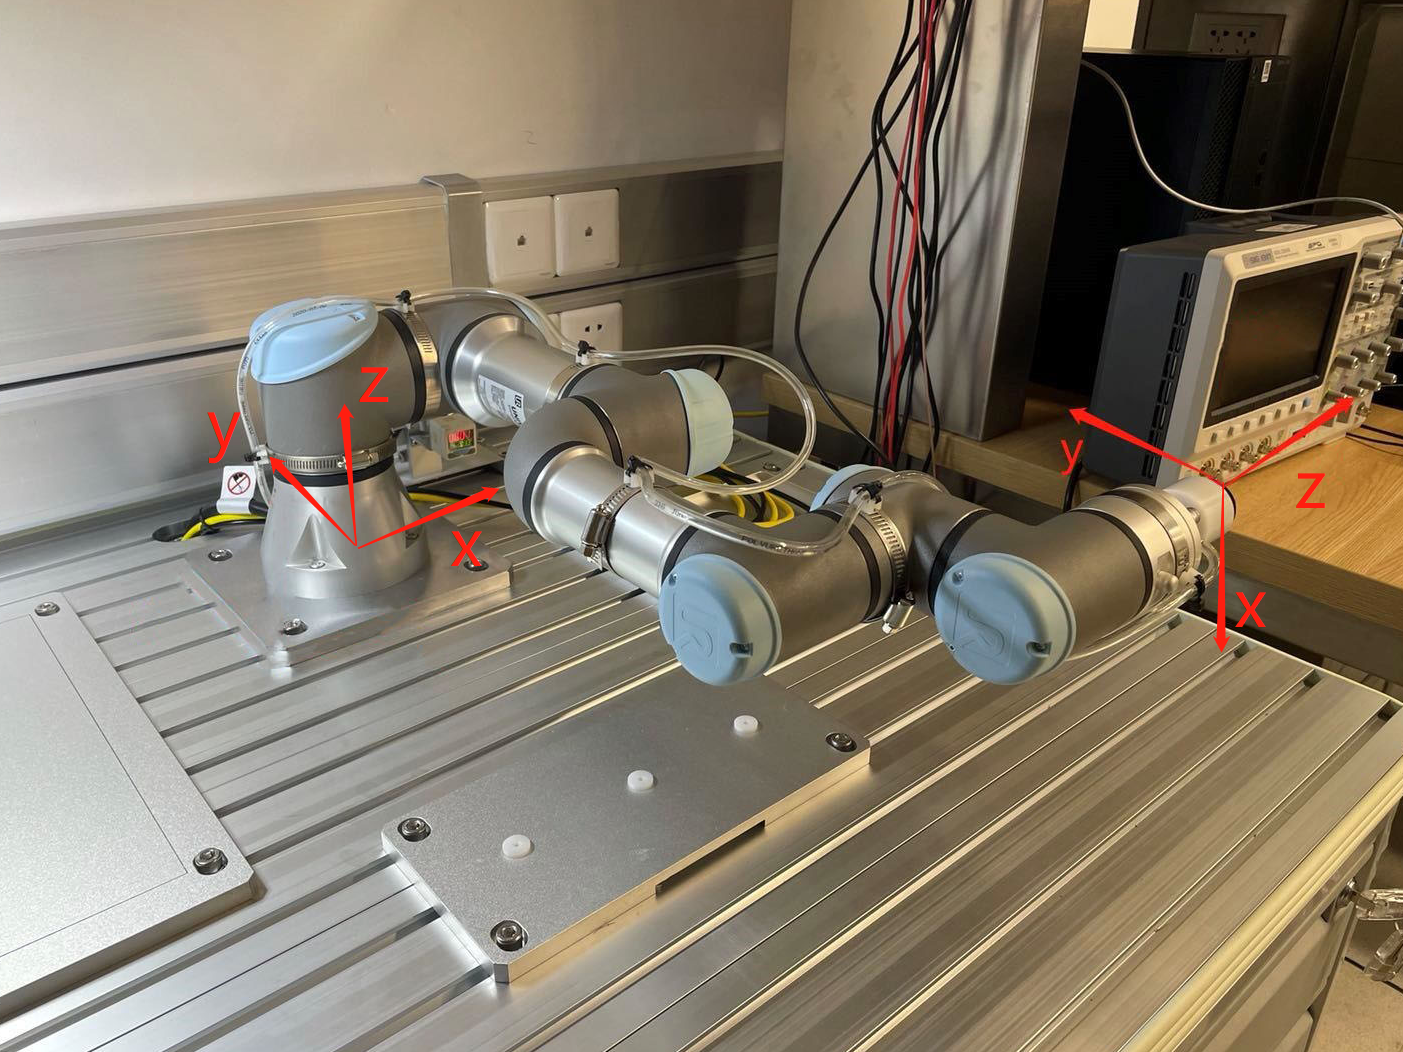
\includegraphics[height=3.4in]{image/lab4_zero_config.jpg}
	\caption{\figlbl{UR3e_zero_config} “zero” configuration and frame placement for UR3e.}
\end{figure}

Moreover, please note that in this lab, all the UR3e robots have a pre-defined zero configuration. The pose shown in \figref{UR3e_zero_config} is \textbf{NOT the TRUE zero configuration} according to the teach pendant. In this pose (\figref{UR3e_zero_config}), you would read the following joint angles from \textbf{the teach pendant}:

\begin{center}
\begin{tabular}{ |c|c|c|c|c|c| } 
\hline
Joint 1 & Joint 2 & Joint 3 & Joint 4 & Joint 5 & Joint 6\\
\hline
90.0$^{\circ}$ & 0.0$^{\circ}$ & 0.0$^{\circ}$ & -90.0$^{\circ}$ & 0.0$^{\circ}$ & 0.0$^{\circ}$\\ 
\hline
\end{tabular}
\end{center}
In the  \textbf{teach pendant's} zero configuration, (due to how the robot is originally mounted) the robot arm would face the far edge of the table and the wrist joint would point into the table, which is an awkward pose to make measurements and do experiments. Hence, we added some angle offsets in the function script such that:

\begin{lstlisting}
	return_value[0] = theta1 + (0.5*PI)
	return_value[1] = theta2
	return_value[2] = theta3
	return_value[3] = theta4 - (0.5*PI)
	return_value[4] = theta5
	return_value[5] = theta6
\end{lstlisting}

(\textbf{Attention:} Remember in the previous lab, when we enter the angle value
on control panel into python code, the value of base and elbow should be
switched.)

\textbf{Any joint angle measurements from the robot that are passed to your ROS program will be corrected to the “zero” configuration shown in \figref{UR3e_zero_config}.}
In other words, now if you set all the joint of UR3e to zero (zero configuration) in \textbf{ROS}:
\begin{center}
\begin{tabular}{ |c|c|c|c|c|c| } 
\hline
Joint 1 & Joint 2 & Joint 3 & Joint 4 & Joint 5 & Joint 6\\
\hline
0.0$^{\circ}$ & 0.0$^{\circ}$ & 0.0$^{\circ}$ & 0.0$^{\circ}$ & 0.0$^{\circ}$ & 0.0$^{\circ}$\\ 
\hline
\end{tabular}
\end{center}
You would see the UR3e poses as \figref{UR3e_zero_config} showed.

\item The sole purpose of the forward kinematics algorithm is to estimate the end-effector's pose (orientation and position) with respect to the base frame given a set of joint angles. This information can be packed and calculated in a “homogeneous transformation matrix” as taught by Lynch \& Park in \textit{Modern Robotics}:
\begin{center}
\begin{equation*}
T(\theta) = e^{[S_1]\theta_1} e^{[S_2]\theta_2}...... e^{[S_{n-1}]\theta_{n-1}} e^{[S_n]\theta_n} M
\end{equation*}
\end{center}

While our objective is to solve for the homogeneous transformation matrix $T(\theta)$ of the “motion” caused by certain joint angle configurations, there are seven matrices we need to specify:
    \begin{itemize}
    \item The screw axes $S_1$ to $S_6$ (we have six here because UR3e has six joints) expressed in the base frame, corresponding to the joint motions when the robot is at its zero configuration (see \figref{UR3e_zero_config})
    \item The end-effector pose M (a 4x4 homogeneous transformation matrix) with respect to the base frame, corresponding to the zero configuration
    \end{itemize}
A screw axis S can be represented by $S=(\omega,v)$, where the $\omega$ is the joint axis defined by the \textbf{right hand rule} (\figref{hand}). $v$ can be computed by $v= -\omega \times q$, where q is the displacement (position) of the joint center with respect to the base frame.
\begin{figure}[t]
	\centering
		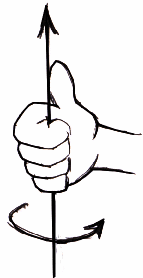
\includegraphics[scale=1]{image/lab4_hand.png}
	\caption{\figlbl{hand}The "right hand rule"}
\end{figure}

\item Using the symbolic toolbox of Matlab or Python, find the closed form solution of $T_{06}$.  You should note how long and complex the solution is due to the contribution of each joint's motion.  Additionally, calculate the 6 matrices defined by $e^{[S_1]\theta_1}$ through $e^{[S_6]\theta_6}$.

\item To aid in your calculations, several figures have been included.
\begin{itemize}
    \item \figref{UR3SA} shows the screw axes and direction of rotation (use the right rule) for each joint.
    \item \figref{UR3JC} shows the joint centers to aid in locating your $q$ values.
    \item \figref{UR3Dim} shows the dimensions of all of the links of the UR3e.
    \item \figref{EEoffset} shows the dimensions of the end effector including the aluminum plate and suction gripper.
\end{itemize}

\end{enumerate}

\subsection{Implementation on UR3e}
\begin{enumerate}
\item Copy \textbf{lab4pkg\_fk} into ``\textbf{src}" directory of your catkin directory.  Don't forget ``\textbf{source devel/setup.bash}" when you open a new terminal.  Then from your base catkin\
directory run ``\textbf{catkin\_make}" and if you receive no errors you copied your lab3 starter code correctly.  Also so that ROS registers this new package ``\textbf{lab4pkg\_fk}",
run ``\textbf{rospack list}" and you should see \textbf{lab4pkg\_fk} as one of the many packages.
\item You will notice that in \textbf{lab4pkg\_fk/scripts} there are now three *.py files.  \textbf{lab4\_exec.py} is the main() code, \textbf{lab4\_func.py} defines the important
forward kinematic functions. \textbf{lab4\_header.py} defines the header files.  We divide them up in this fashion for clarity.  In this lab you will be mainly editing
\textbf{lab4\_func.py}.  You can of course change \textbf{lab4\_exec.py} but most of its functionality has already been given to you.  Study the code and comments in
\textbf{lab4\_exec.py} and \textbf{lab4\_func.py} to see what the starter code is doing and what parts you are going to need to change. Your job is to add the code in the function \textbf{Get\_MS()} that correctly populates the six screw axes $S_1$ to $S_6$ as well as the transformation matrix M.  The Python code uses the ``numpy" module to create and multiply matrixes; meanwhile, the matrix exponential ``expm()" is achieved by including the ``Scipy" module.  Then, with the S and M values you populated, write the code in function \textbf{lab\_fk()} that generates and prints the homogeneous transformation matrix $T(\theta)$.

\item Once your code is finished, run it using ``\textbf{rosrun lab4pkg\_fk lab4\_exec.py [theta1] [theta2] [theta3] [theta4] [theta5] [theta6]}" with all angles in
degrees - e.g. \textbf{rosrun lab4pkg\_py lab4\_exec.py 0 90 45 0 -90 105}.  Remember that in another command prompt you should have first run roscore and drivers using
``\textbf{roslaunch ur\_robot\_driver ur3e\_bringup.launch}".

\item For in-person students, you should measure the x,y,z position of the end-effector using the provided ruler and square.  For students using the simulation, it is not possible to measure this way, so we must use another method.  A simple way is to use some of the ROS commands we learned before: ``\textbf{rostopic echo /gripper/position -n 1}".  These values are being calculated differently and so there will be small differences between this value and your calculations.
\item You should verify that your code works by selecting a variety of poses that will test the full range of motion.  Your TA will not be providing you test angles, so you should make use of the joint limits provided in Section \ref{sec:physical}.

\end{enumerate}
\subsection{Comparison}
\begin{enumerate}
\item Your TA will select two sets of joint angles $\left\{\theta_1,\theta_2,\theta_3,\theta_4,\theta_5,\theta_6\right\}$ when you demonstrate\
your working ROS program.  
\item Run your ROS node and move the UR3e to each of these configurations.  With a ruler and square (or the appropriate ROS command for the simulation),  measure the x,y,z position vector of the center of the gripper for each set of angles.  Call these vectors $r_1$ and $r_2$ for the first and second sets of joint angles, respectively.

\item Compare these measurements to the translation vector calculated by your ROS node.  
Call these calculated vectors $d_1$ and $d_2$.	

\item For each set of joint angles, Calculate the error between the measured and calculated kinematic solutions.  We will consider the error to be the magnitude of the distance between the measured center of the gripper and the location predicted by the forward kinematic equation:
\[
error_1 = \left\| r_1 - d_1 \right\| = \sqrt{(r_{1x}-d_{1x})^2 + (r_{1y}-d_{1y})^2 + (r_{1z}-d_{1z})^2}.
\]
A similar expression holds for $error_2$.
\end{enumerate}


\section{Report}
Each student will submit a lab report using the guidelines given in the “ECE 470: How to Write a Lab Report” document.  Please be aware of the following:
\begin{itemize}
    \item Lab reports will be submitted online at \href{https://learn.intl.zju.edu.cn/}{Blackboard}.
    \item The report will be due \textbf{2} weeks after your lab session for Lab 3.  Exact times and dates can be seen on \href{https://learn.intl.zju.edu.cn/}{Blackboard}.
\end{itemize}


Your lab report should include the following:
\begin{itemize}
\item Explain how you determined $\mathcal{S}_{1}$ thru $\mathcal{S}_{6}$ and $\textbf{M}$ - include figures as needed.
\item Include a figure that shows all frames and axes used.
\item Include a table of all $\omega$ and $q$ used and the $v$ derived.
\item Figures should be your own creation and not copies of the lab manual.

 \item Use Matlab or Python's symbolic toolbox to generate the final homogeneous transform $T_{06}$ as a function of $\left(\theta_{1},\theta_{2},\theta_{3},\theta_{4},\theta_{5},\theta_{6}\right)$.  As this is too cumbersome to include in your report, include $e^{[S_1]\theta_1}$ through $e^{[S_6]\theta_6}$ in your report (do not use screenshots).

\item Substitute in your given joint angles into your symbolic solution to verify it.
\item For each test point, include:
    \begin{itemize}
        \item The given $\left(\theta_{1},\theta_{2},\theta_{3},\theta_{4},\theta_{5},\theta_{6}\right)$
        \item The calculated $d$ and measured $r$ vectors
        \item The scalar error
        \item The output of your symbolic solution
    \end{itemize}
    \item Include a brief discussion of sources of error.
\end{itemize}
Unless your TA gives other guidance, include the following as appendices:
\begin{itemize}
    \item Your $\textbf{lab4\_func.py}$ code (and $\textbf{lab4\_exec.py}$ if it was edited).
    \item Your Matlab or Python code used to calculate the symbolic $T_{06}$.
\end{itemize}


\section{Demonstration}
Demonstrations of your working code will either be done in-person or over Zoom.  They will be done live (i.e. no recordings) with your lab section TA.  Demos are due \textbf{2} weeks after your lab session.\\

The default method of demonstrating your work will be via the simulation.  While we want to encourage in-person students to run their code on the real robot, due to time limitations, this may be difficult to do with your TA by the due date.  You can always run it for your own satisfaction at another time.
\subsection{Demo Process}
Your TA will require you to run your program twice, each time with a different set of joint variables.


\section{Grading}
\begin{itemize}
\item 80 points, successful demonstration.
\item 20 points, individual report.  
\end{itemize}


% \section{Tentative Due Dates - Fall 2020}
% The exact date and time will depend on your lab section and can be found on \href{www.gradescope.com}{GradeScope}.
% \subsection{Group A}
% \begin{itemize}
%     \item Demonstration - Week of October 19
%     \item Report - Week of October 26
% \end{itemize}

% \subsection{Group B}
% \begin{itemize}
%     \item Demonstration - Week of October 26
%     \item Report - Week of November 2
% \end{itemize}

\section{Preparation for Lab 5}
Lab 5 will cover inverse kinematics.  In class you will mostly focus on numerical inverse kinematics, but we will be using analytical inverse kinematics - i.e. we will use geometry and constraints to find a closed form solution to the problem.\\
Suggested Reading:
\begin{itemize}
    \item Chapter 6 of \textit{Modern Robotics} provides multiple examples of inverse kinematics solutions. Especially Section 6.1.
    \item Chapter 3 of \textit{Robot Modeling and Control}, by M. Spong, S. Hutchinson and M Vidyasagar (Wiley and Sons, 2005).  Especially Section 3.3.3.  (A version of this text is available online.)
\end{itemize}


\begin{figure}[t]
	\centering
		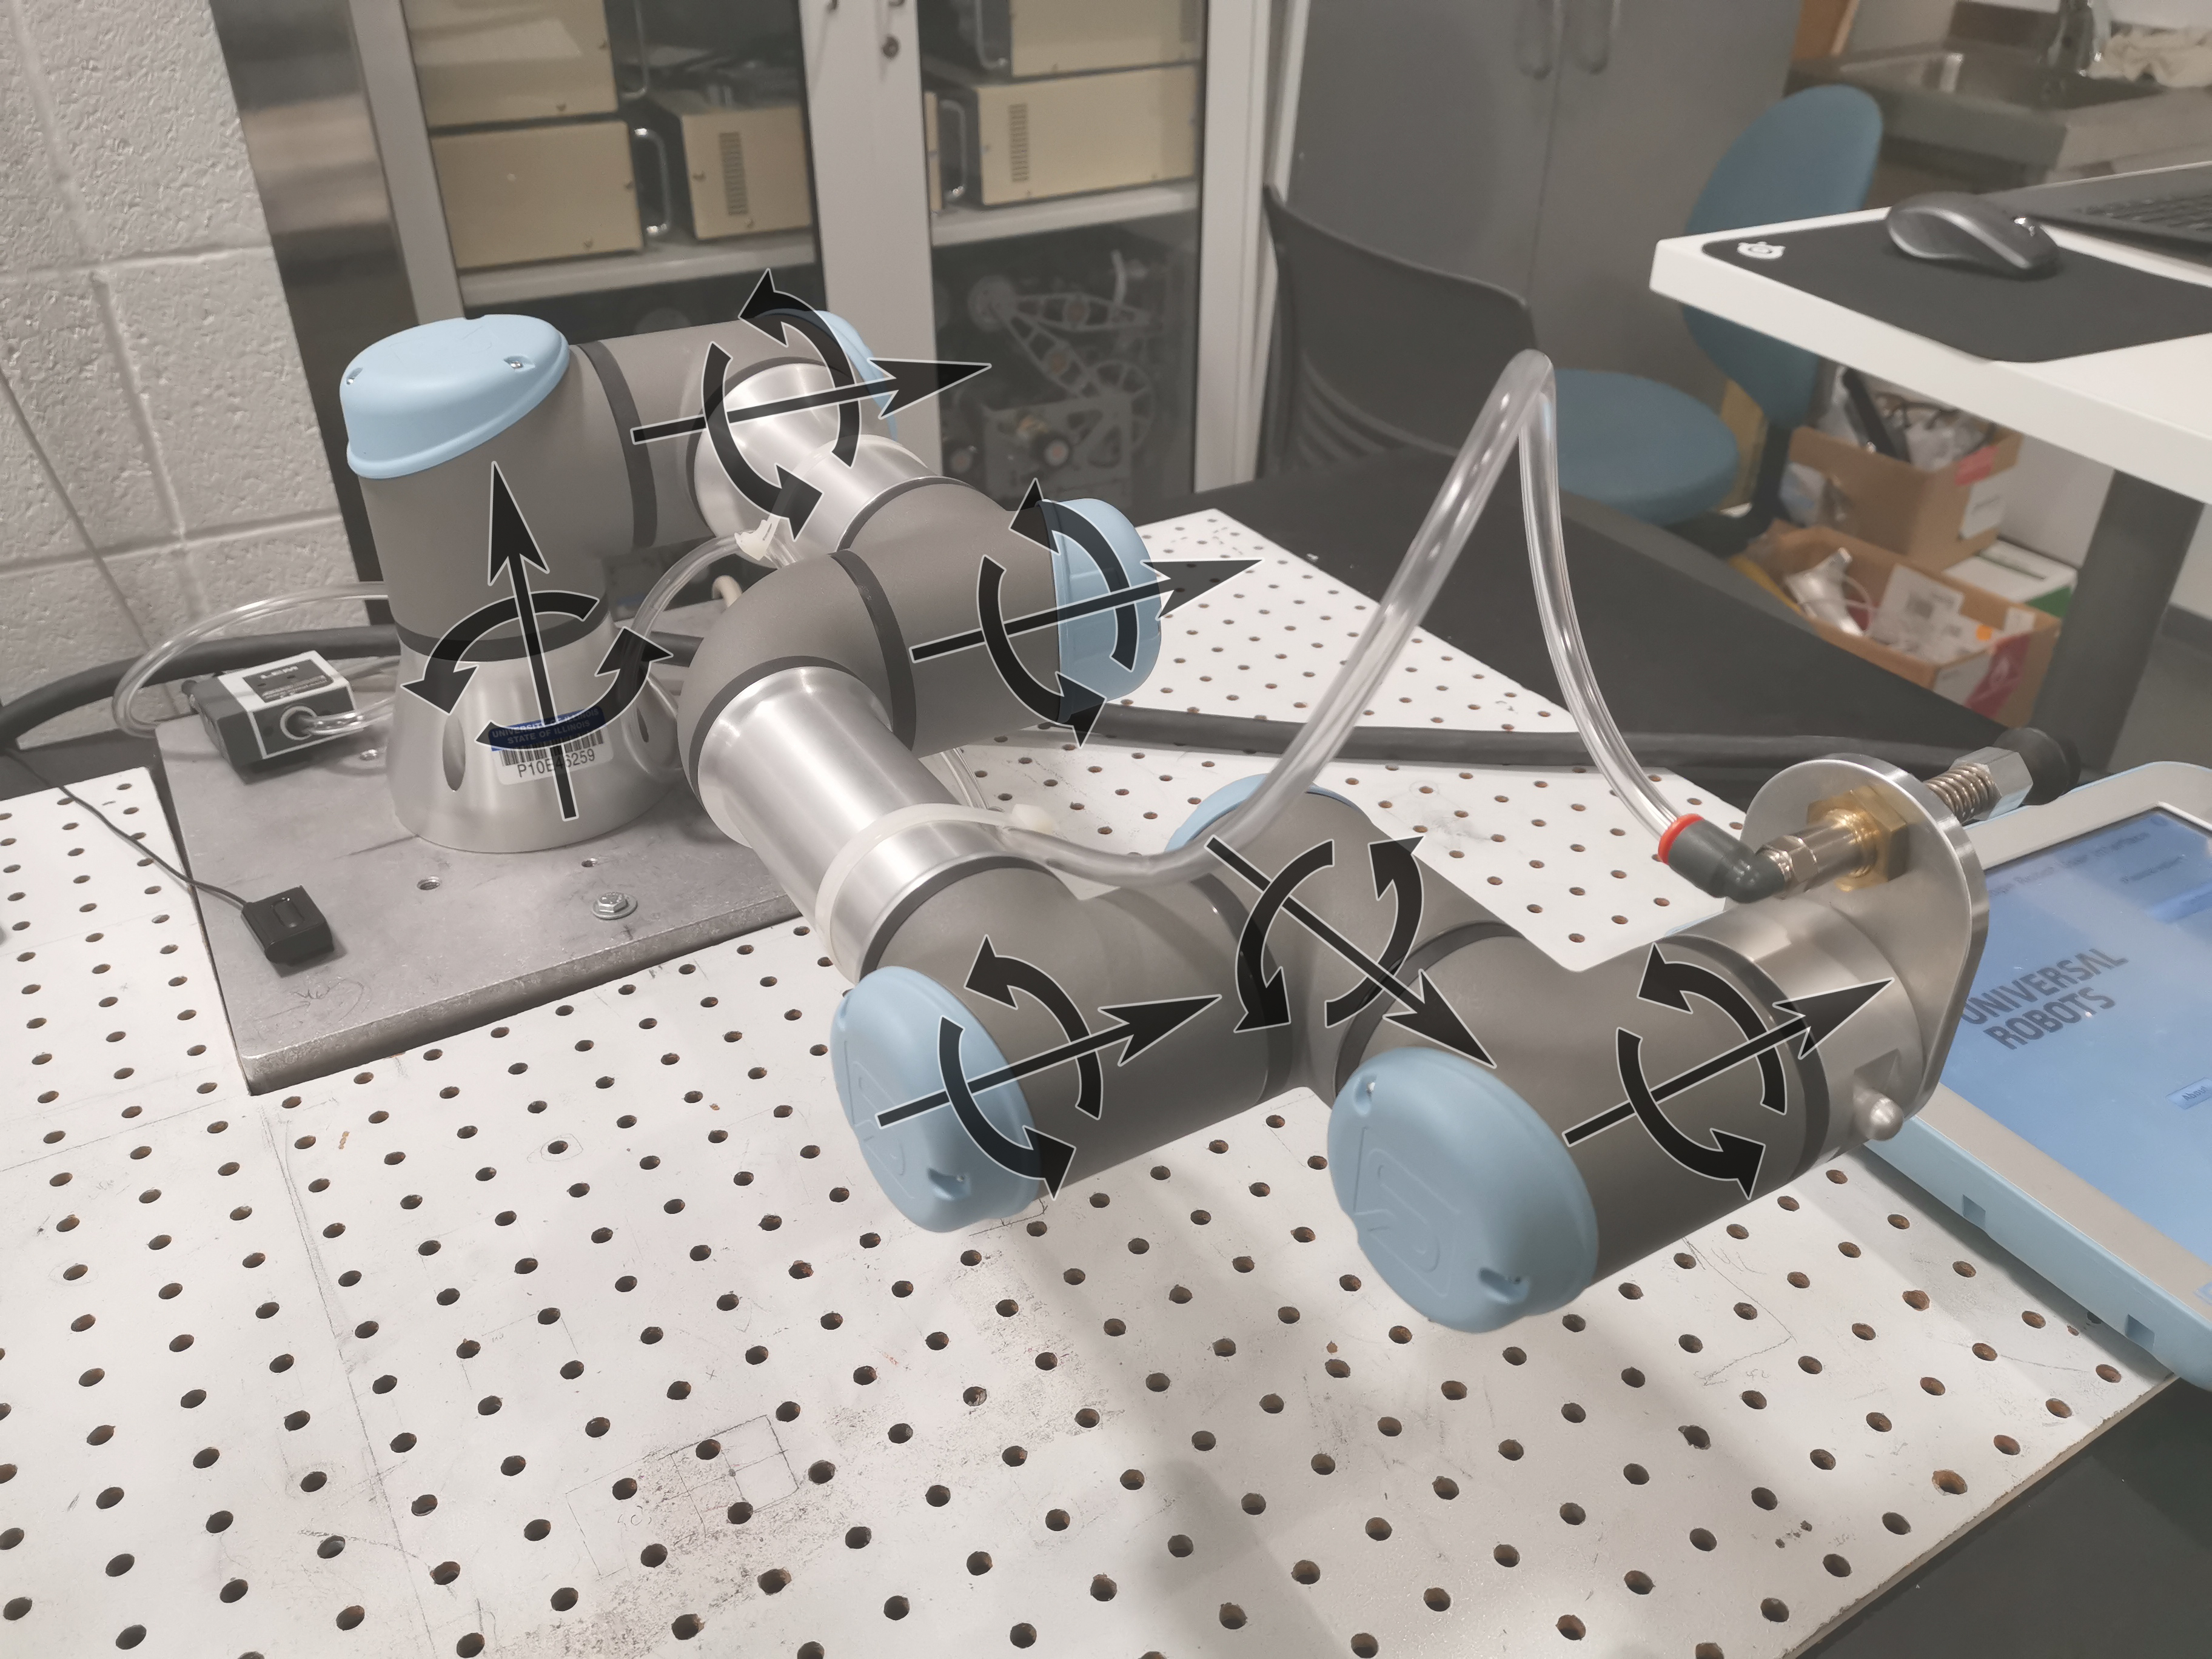
\includegraphics[height=3.4in]{image/lab4_ur3_forwardkin1.jpg}
	\caption{\figlbl{UR3SA} Screw axes on UR3e.}
\end{figure}

\begin{figure}[t]
	\centering
		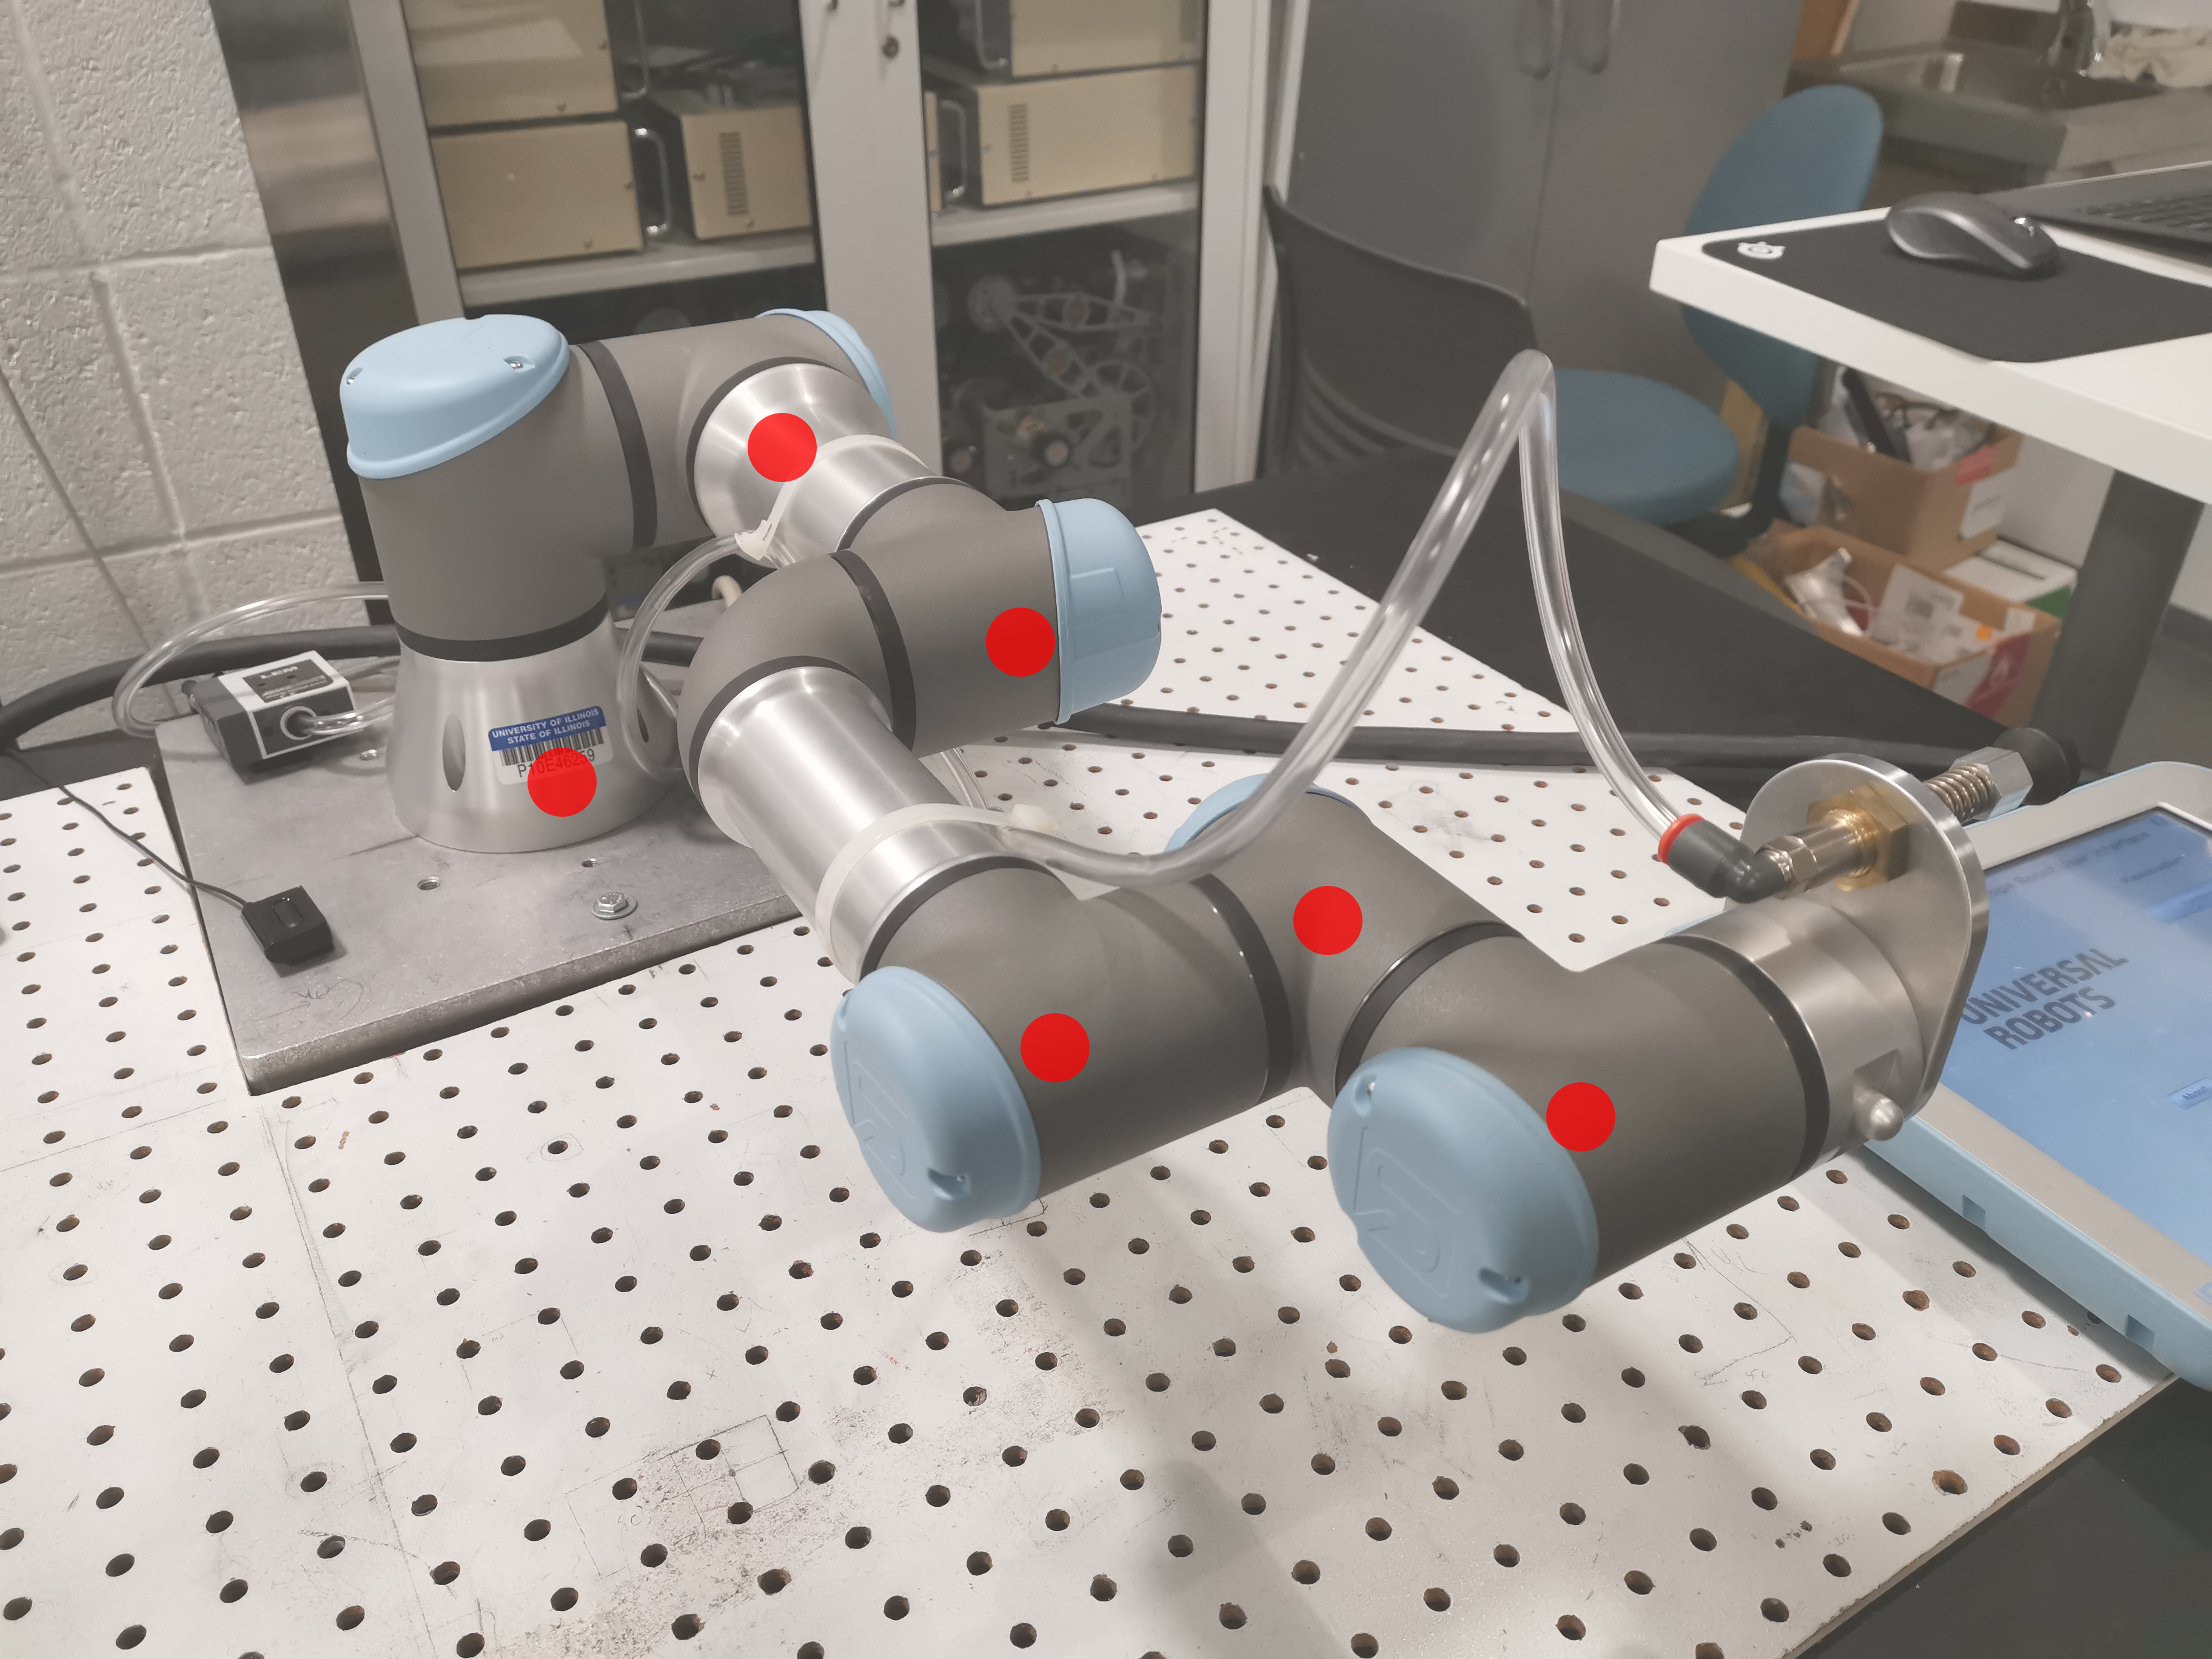
\includegraphics[height=3.4in]{image/lab4_ur3_forwardkin.jpg}
	\caption{\figlbl{UR3JC} Joint center locations on UR3e.}
\end{figure}

\begin{figure}[t]
	\centering
		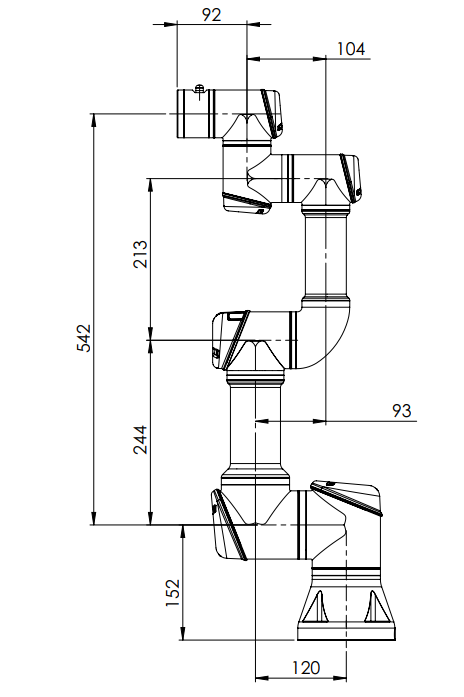
\includegraphics[height=6in]{image/lab4_ur3e_config.png}
	\caption{\figlbl{UR3Dim} Approximate Dimensions of the UR3e in mm. *EACH UR3e IS SLIGHTLY DIFFERENT DUE TO ITS MANUFACTURE TOLERANCE.}
\end{figure}


\begin{figure}[t]
	\centering
		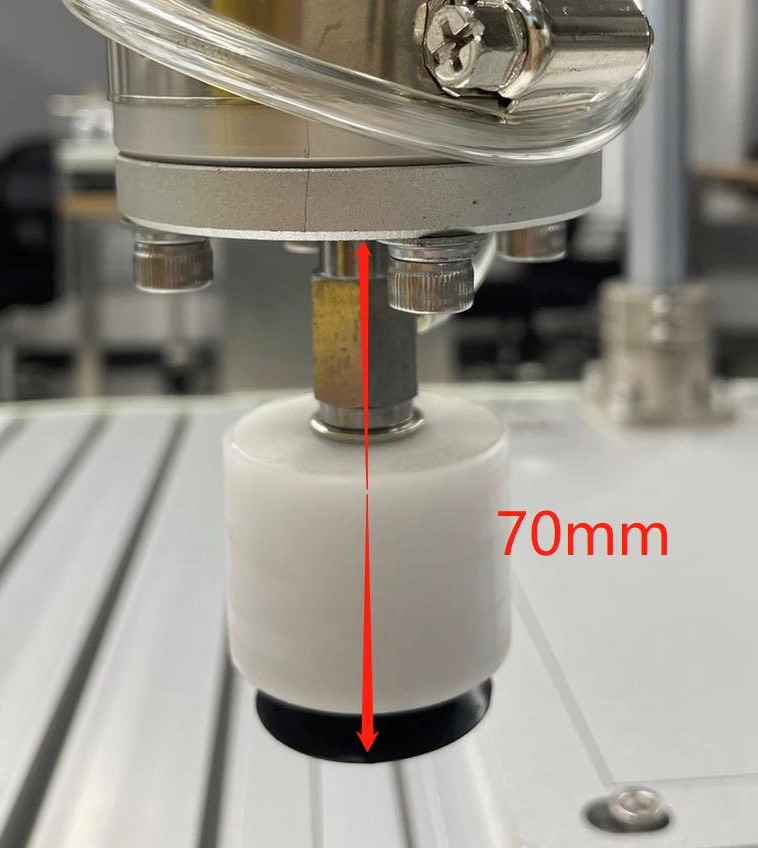
\includegraphics[height=3.5in]{image/lab4_ee_dim.jpg}
	\caption{\figlbl{EEoffset} Approximate Dimensions of the attached end effector plate and suction gripper in mm.}
\end{figure}

\chapter{Inverse Kinematics}
\section{Important}
Read the entire lab before starting and especially the ``Grading" section so you are aware of all due dates and requirements associated with the lab.  Hopefully you are reading this well before your lab section meets as given the compressed schedule, it is very important that you arrive at lab well prepared.  This semester, the more you do prior to your lab session, the more you will get out of the short time you have with the TA.
\section{Objectives}
The purpose of this lab is to derive and implement a solution to the inverse kinematics problem for the UR3e robot.  In this lab we will:
\begin{itemize}
	\item Derive elbow-up inverse kinematic equations for the UR3e
	\item Write a Python function that moves the UR3e to a point in space specified by the user.
\end{itemize}

\section{Reference}
Chapter 6 of \textit{Modern Robotics} provides multiple examples of inverse kinematics solutions.

\section{Tasks}
\subsection{Solution Derivation}
\textbf{Make sure to read through this entire lab before you start deriving your solution.  There are some
needed details not covered in this section.}


Given a desired end-effector position in space $(x_{grip},y_{grip},z_{grip})$ and orientation $\left\{\theta_{yaw},\theta_{pitch}(fixed),
\theta_{roll}(fixed)\right\}$, write six mathematical expressions 
that yield values for each of the joint angles. For the UR3e robot, there are many solutions to the inverse kinematics
problem.  We will implement only one of the \textit{elbow-up} solutions.

\begin{itemize}
\item In the inverse kinematics problems you have examined in class (for 6 DOF arms with spherical wrists), usually the first step is to solve
for the coordinates of the wrist center.  The UR3e does not technically have a spherical wrist center but we will define the wrist center as $z_{cen}$
which equals the same desired z value of the suction cup and $x_{cen}$, $y_{cen}$ are the coordinates of $\theta_6$'s z axis.
In addition, to make the derivation manageable,
add that $\theta_5$ will always be $-90^{\circ}$ and $\theta_4$ is set such that link 7 and link 9 are always parallel to the world x,y plane.   
\begin{figure}[tbp]
	\centering
		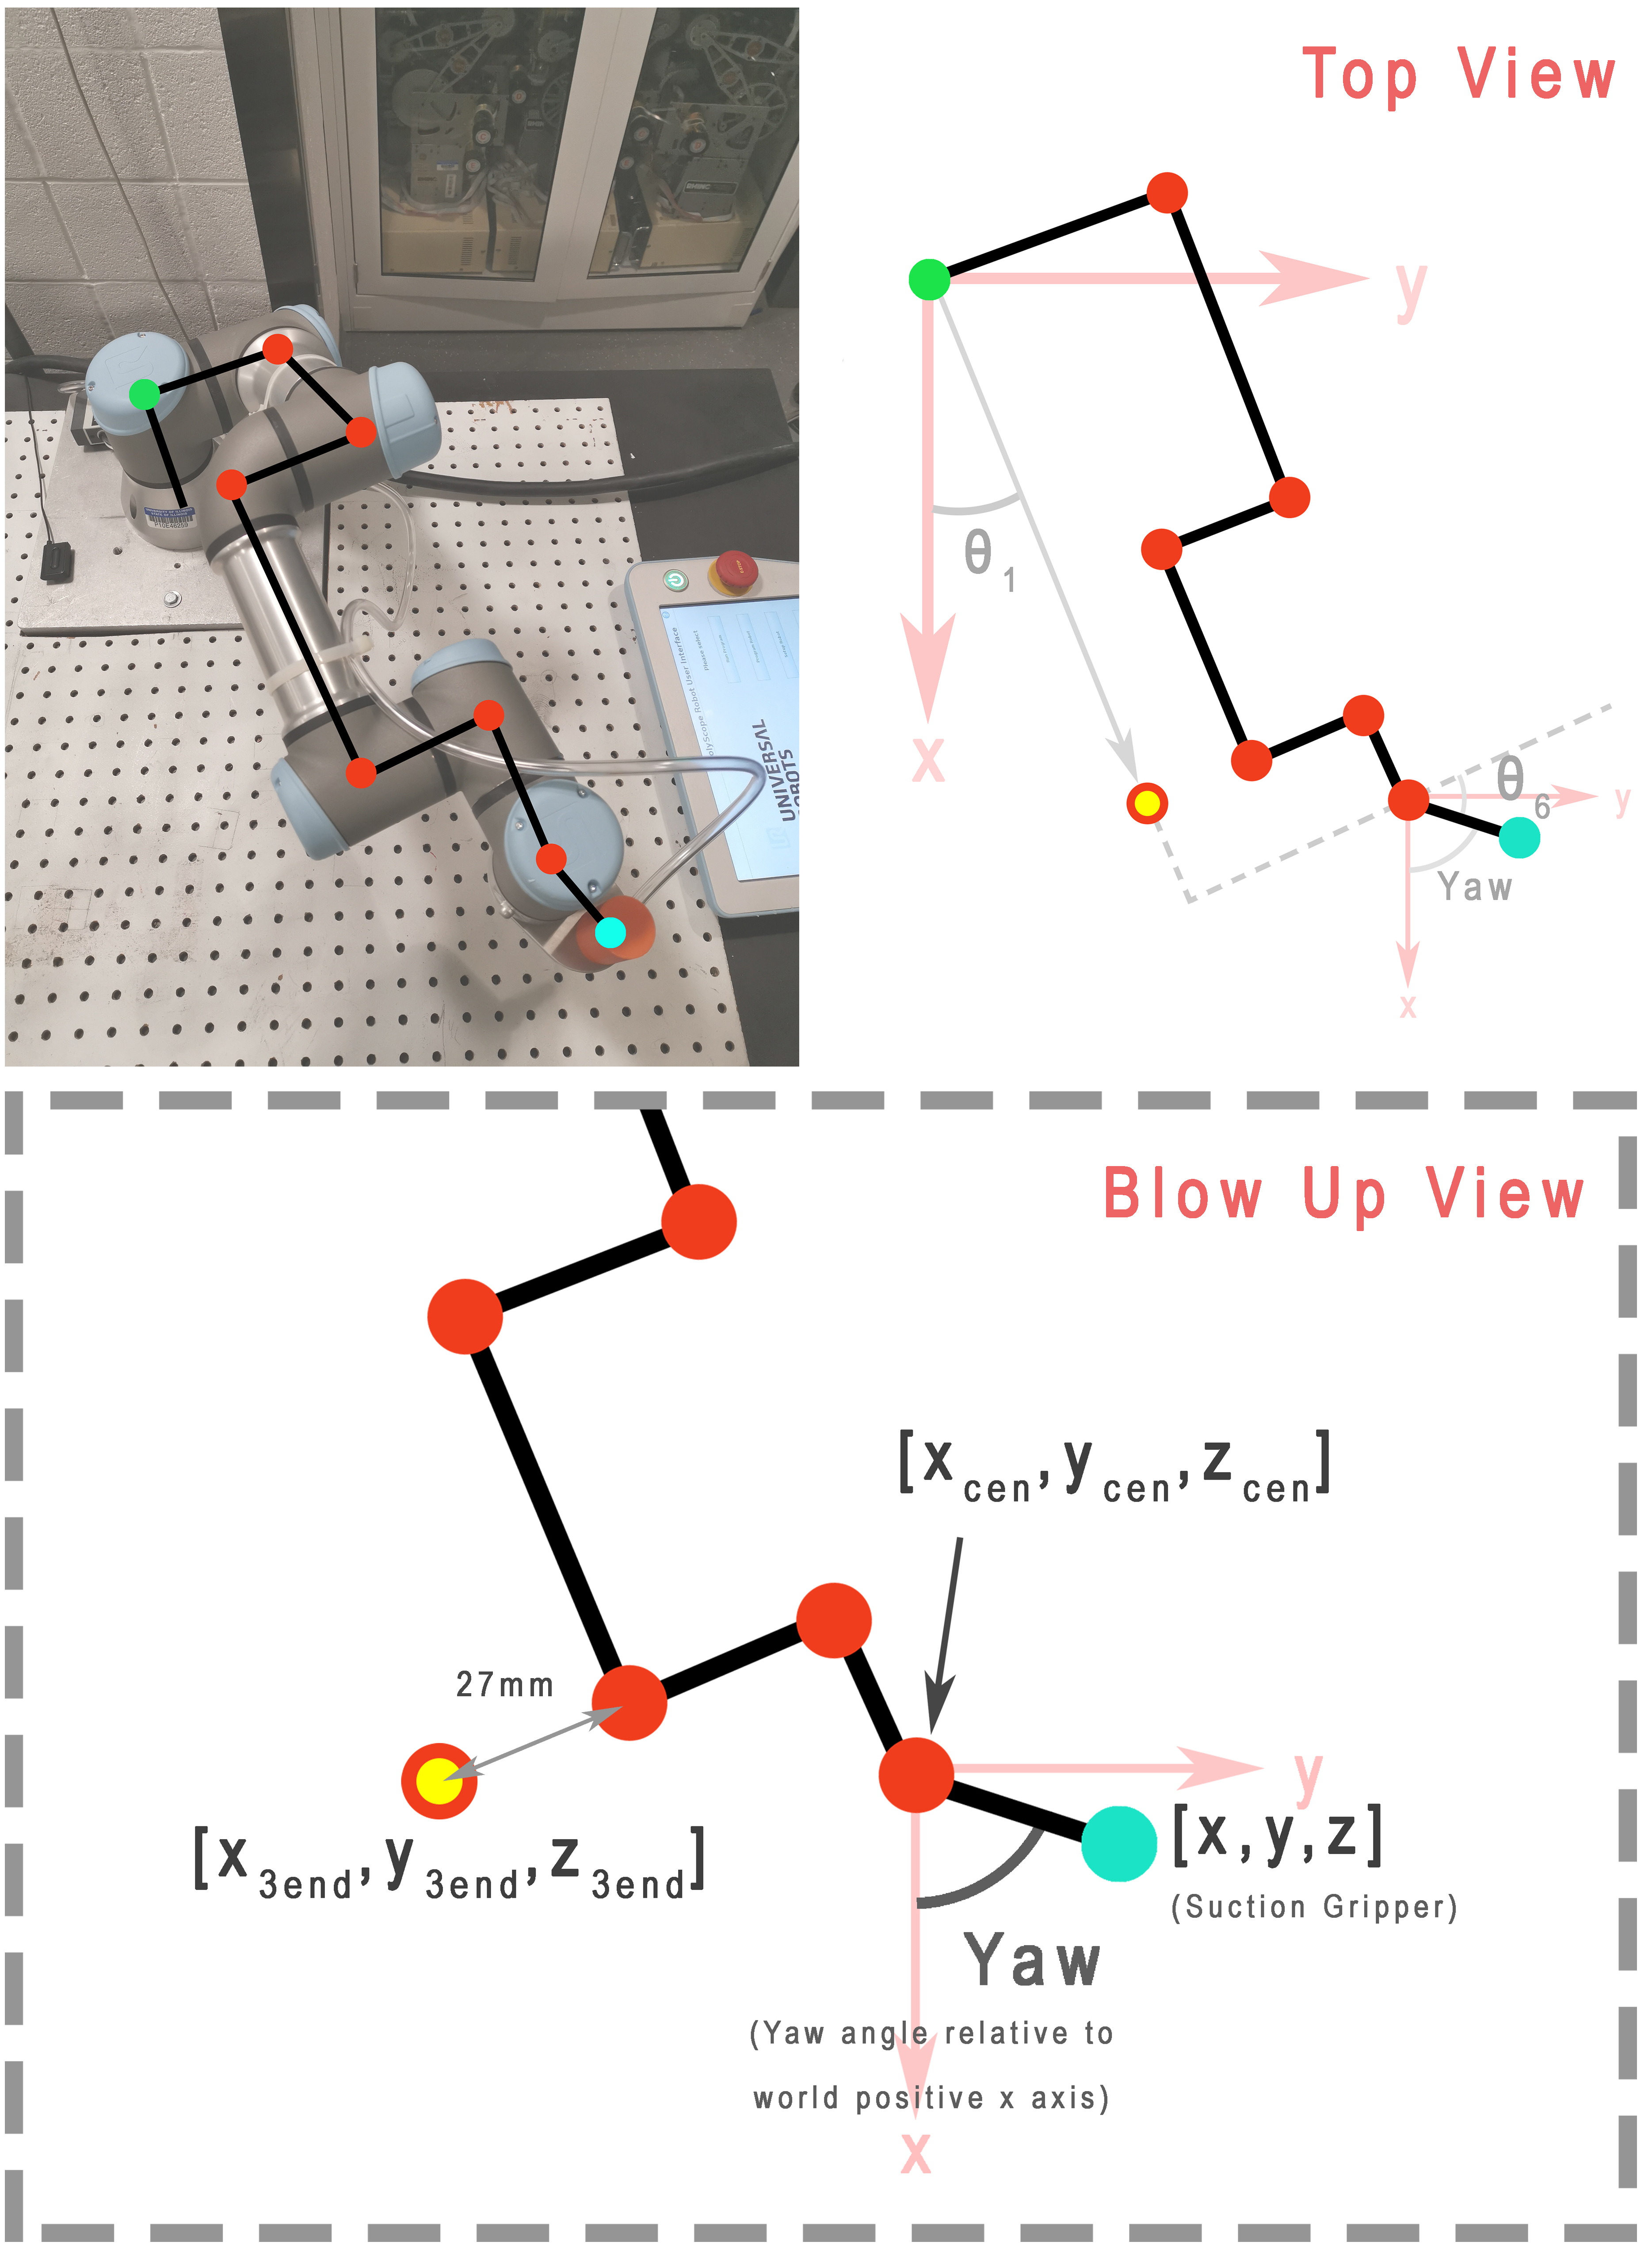
\includegraphics[scale=0.127]{image/lab5_ur3_pre4.jpg}
	\caption{\figlbl{TopView} Top View Stick Pictorial of UR3e. Note that the coordinate frames are in the same direction
	as the World Frame but not at the World frame's origin.  One origin is along the center of joint 1 and the second
	is along the center of joint 6.}
\end{figure}

\begin{figure}[tbp]
	\centering
		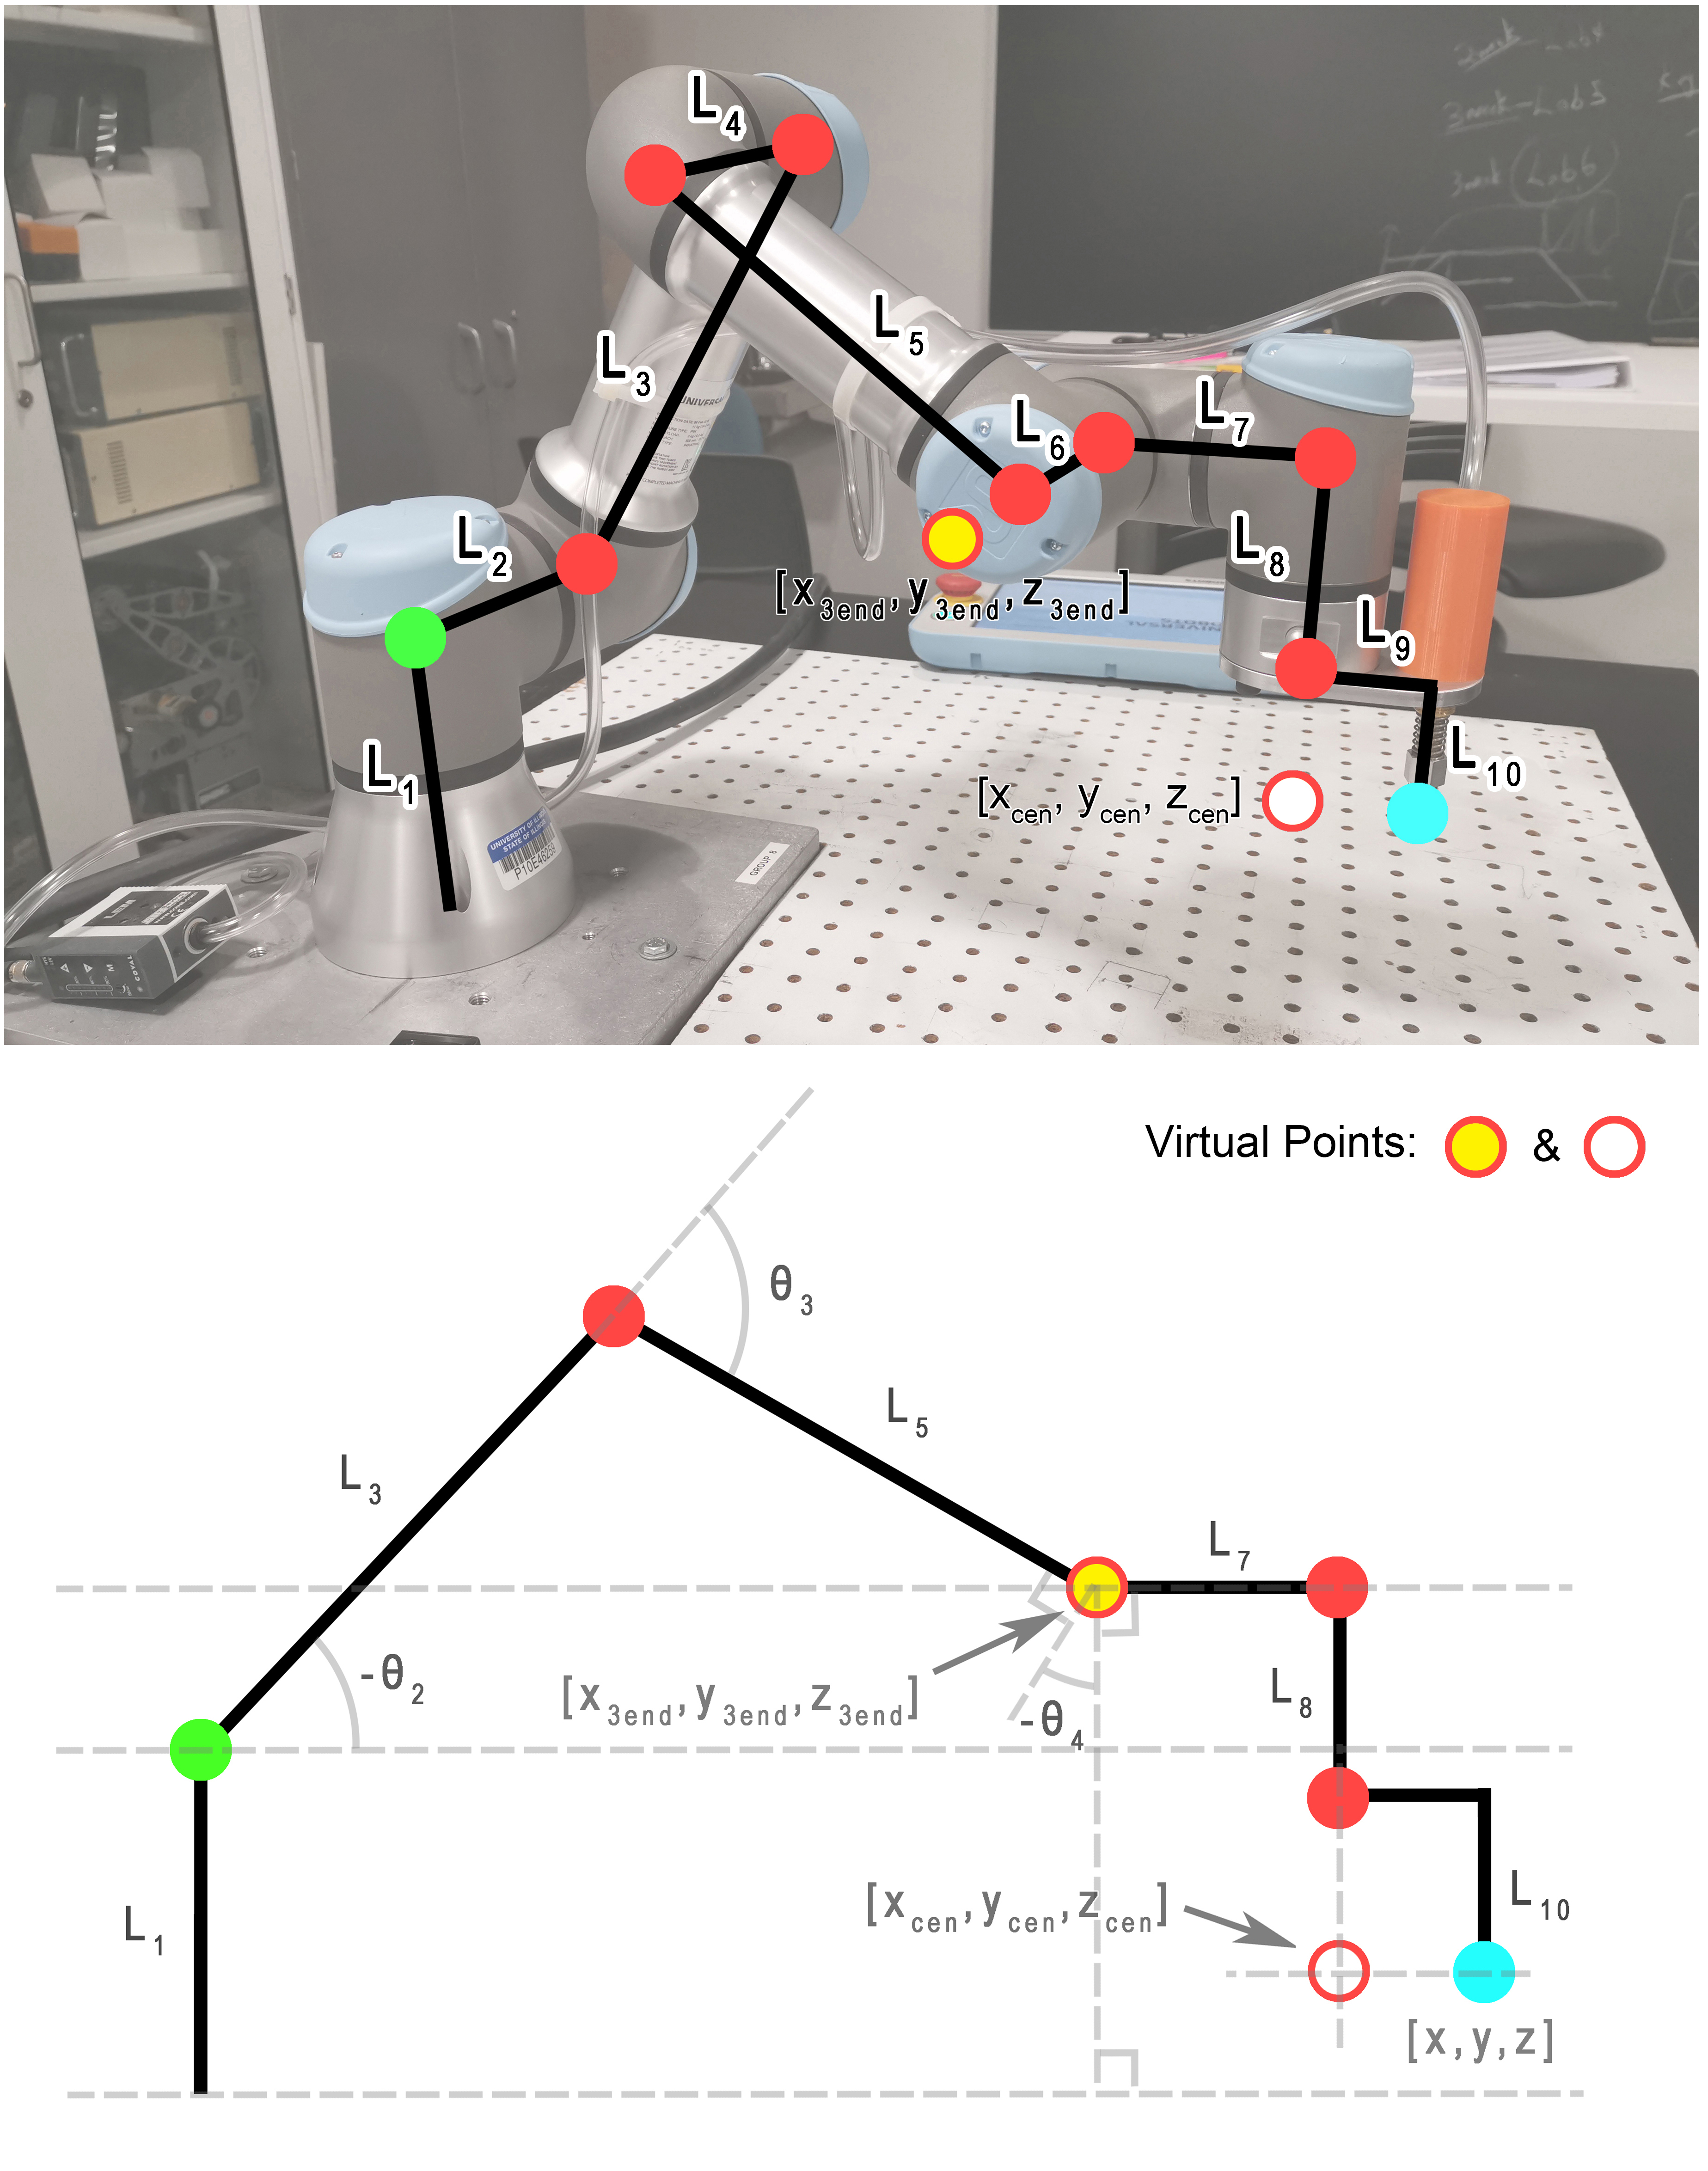
\includegraphics[scale=0.125]{image/lab5_ur3_side3_1_old.jpg}
	\caption{\figlbl{SideView} Side View Stick Pictorial of UR3e.}
\end{figure}

\item Solve the inverse kinematics problem in the following order:
\begin{enumerate}
	\item $x_{cen}$, $y_{cen}$, $z_{cen}$, given yaw desired in the world frame and the desired x,y,z of the suction cup. The suction cup aluminum
plate (link 9) has a length of 0.0535 meters from the center line of the suction cup to the center line of joint 6. Remember that this
aluminum plate should always be parallel to the world's x,y plane.  See \figref{SideView}.	
	\item $\theta_1$, by drawing a top down picture of the UR3e, \figref{TopView}, and using $x_{cen}$, $y_{cen}$, $z_{cen}$ that you just calculated.
	\item $\theta_6$, which is a function of $\theta_1$ and yaw desired.  Remember that when $\theta_6$ is equal to zero the suction cup aluminum plate
is parallel to link 4 and link 6.
  	\item $x_{3end}$, $y_{3end}$, $z_{3end}$ is a point off of the UR3e but lies along the link 6 axis, \figref{TopView}.  For example if $\theta_1 = 0^{\circ}$ then $y_{3end} = 0$.
If $\theta_1 = 90^{\circ}$ then $x_{3end} = 0$.  First use the top down view of the UR3e to find $x_{3end}$, $y_{3end}$.  One way is to choose an appropriate
coordinate frame at $x_{cen}$, $y_{cen}$ and find the translation matrix that rotates and translates that coordinate frame to the base frame.  
Then find the vector in the coordinate frame you chose at $x_{cen}$, $y_{cen}$ that points from $x_{cen}$, $y_{cen}$ to $x_{3end}$, $y_{3end}$.
Simply multiply this vector by your translation matrix to find the world coordinates at $x_{3end}$, $y_{3end}$.  For $z_{3end}$ create a view of
the UR3e, \figref{SideView}, that is a projection of the robot onto a plane perpendicular to the x,y world frame and rotated by $\theta_1$ about
the base frame.  Call this the side view.  Looking at this side view you will see that $z_{3end}$ is $z_{cen}$ offset by a constant.    
	\item $\theta_2$, $\theta_3$ and $\theta_4$, by using the same side view drawing just drawn above to find $z_{3end}$, \figref{SideView}.
Now that $x_{3end}$, $y_{3end}$, $z_{3end}$ have
been found use sine, cosine and the cosine rule to solve for partial angles that make up $\theta_2$, $\theta_3$ and $\theta_4$.  Hint:  In this side view, a parallel to the base construction line through joint 2
and a parallel to the base construction line through joint 4 are helpful in finding the needed partial angles.       		
\end{enumerate}
\end{itemize}

\subsection{Implementation}
Implement the inverse kinematics solution by writing a Python function to receive world frame coordinates $(x_{Wgrip},y_{Wgrip},z_{Wgrip},yaw_{Wgrip})$, compute the desired
joint variables $\left\{\theta_1,\theta_2,\theta_3,\theta_4,\theta_5,\theta_6\right\}$, and command the UR3e to move to that pose
using functions written in Lab4.

\section{Procedure}
\begin{itemize}
	\item Copy \textbf{lab5pkg\_ik} to your workspace.  You will notice that there are three .py files.  
\textbf{lab5\_exec.py}, \textbf{lab5\_func.py} and \textbf{lab5\_header.py}.  The \textbf{lab5\_func.py} file again will be compiled into a library so that future labs can easily call the inverse kinematic
function.  Like Lab 4, most of the needed code is given to you in \textbf{lab5\_exec.py}.  Your main job will be to add all the inverse kinematic equations to
\textbf{lab5\_func.py}. Please refer to the intermediate steps below to perform the inverse kinematic calculations.  If you look
at \textbf{lab5\_header.py} it includes \textbf{lab5\_header.py}.  This allows you to call the functions you created in \textbf{lab5\_func.py}.

    \item Once your code is finished, run it using ``\textbf{rosrun lab5pkg\_ik lab5\_exec.py [x] [y] [z] [yaw(degrees)]}" - e.g. ``\textbf{rosrun lab5pkg\_ik lab5\_exec.py 0.1 0.1 0.15 90}".  Remember to run drivers that in another command prompts at first. 

    \item For in-person students, you should measure the x,y,z position of the end-effector using the provided ruler and square.  For students using the simulation, it is not possible to measure this way, so we must use another method.  A simple way is to use some of the ROS commands we learned before: ``\textbf{rostopic echo /gripper/position -n 1}".  These values are being calculated differently and so there will be small differences between this value and your calculations.
    
    \item You should verify that your code works by selecting a variety of poses that will test the full range of motion.  Your TA will not be providing you test points.

	\item In your code (This is repeating the derivation steps above):
\begin{enumerate}	
	\item Establish the world coordinate frame (frame $w$) centered at the corner of the UR3e's base shown in \figref{frames}.
The $x_w$ and $y_w$ plane should correspond to the surface of the table, with the $x_w$ axis parallel to the sides of the
table and the $y_w$ axis parallel to the front and back edges of the table.  Axis $z_w$ should be normal to the table surface,
with up being the positive $z_w$ direction and the surface of the table corresponding to $z_w=0$.\\
We will solve the inverse kinematics problem in the base frame (frame 0), so we will immediately convert the coordinates entered by
the user to base frame coordinates.  Write three equations relating coordinates $(x_{Wgrip},y_{Wgrip},z_{Wgrip})$ in the world frame to coordinates
$(x_{grip},y_{grip},z_{grip})$ in the base frame of the UR3e.  
  \begin{eqnarray*}
	x_{grip}(x_{Wgrip},y_{Wgrip},z_{Wgrip}) =\\
	y_{grip}(x_{Wgrip},y_{Wgrip},z_{Wgrip}) =\\
	z_{grip}(x_{Wgrip},y_{Wgrip},z_{Wgrip}) =
	\end{eqnarray*}

\begin{figure}[h]
	\centering
		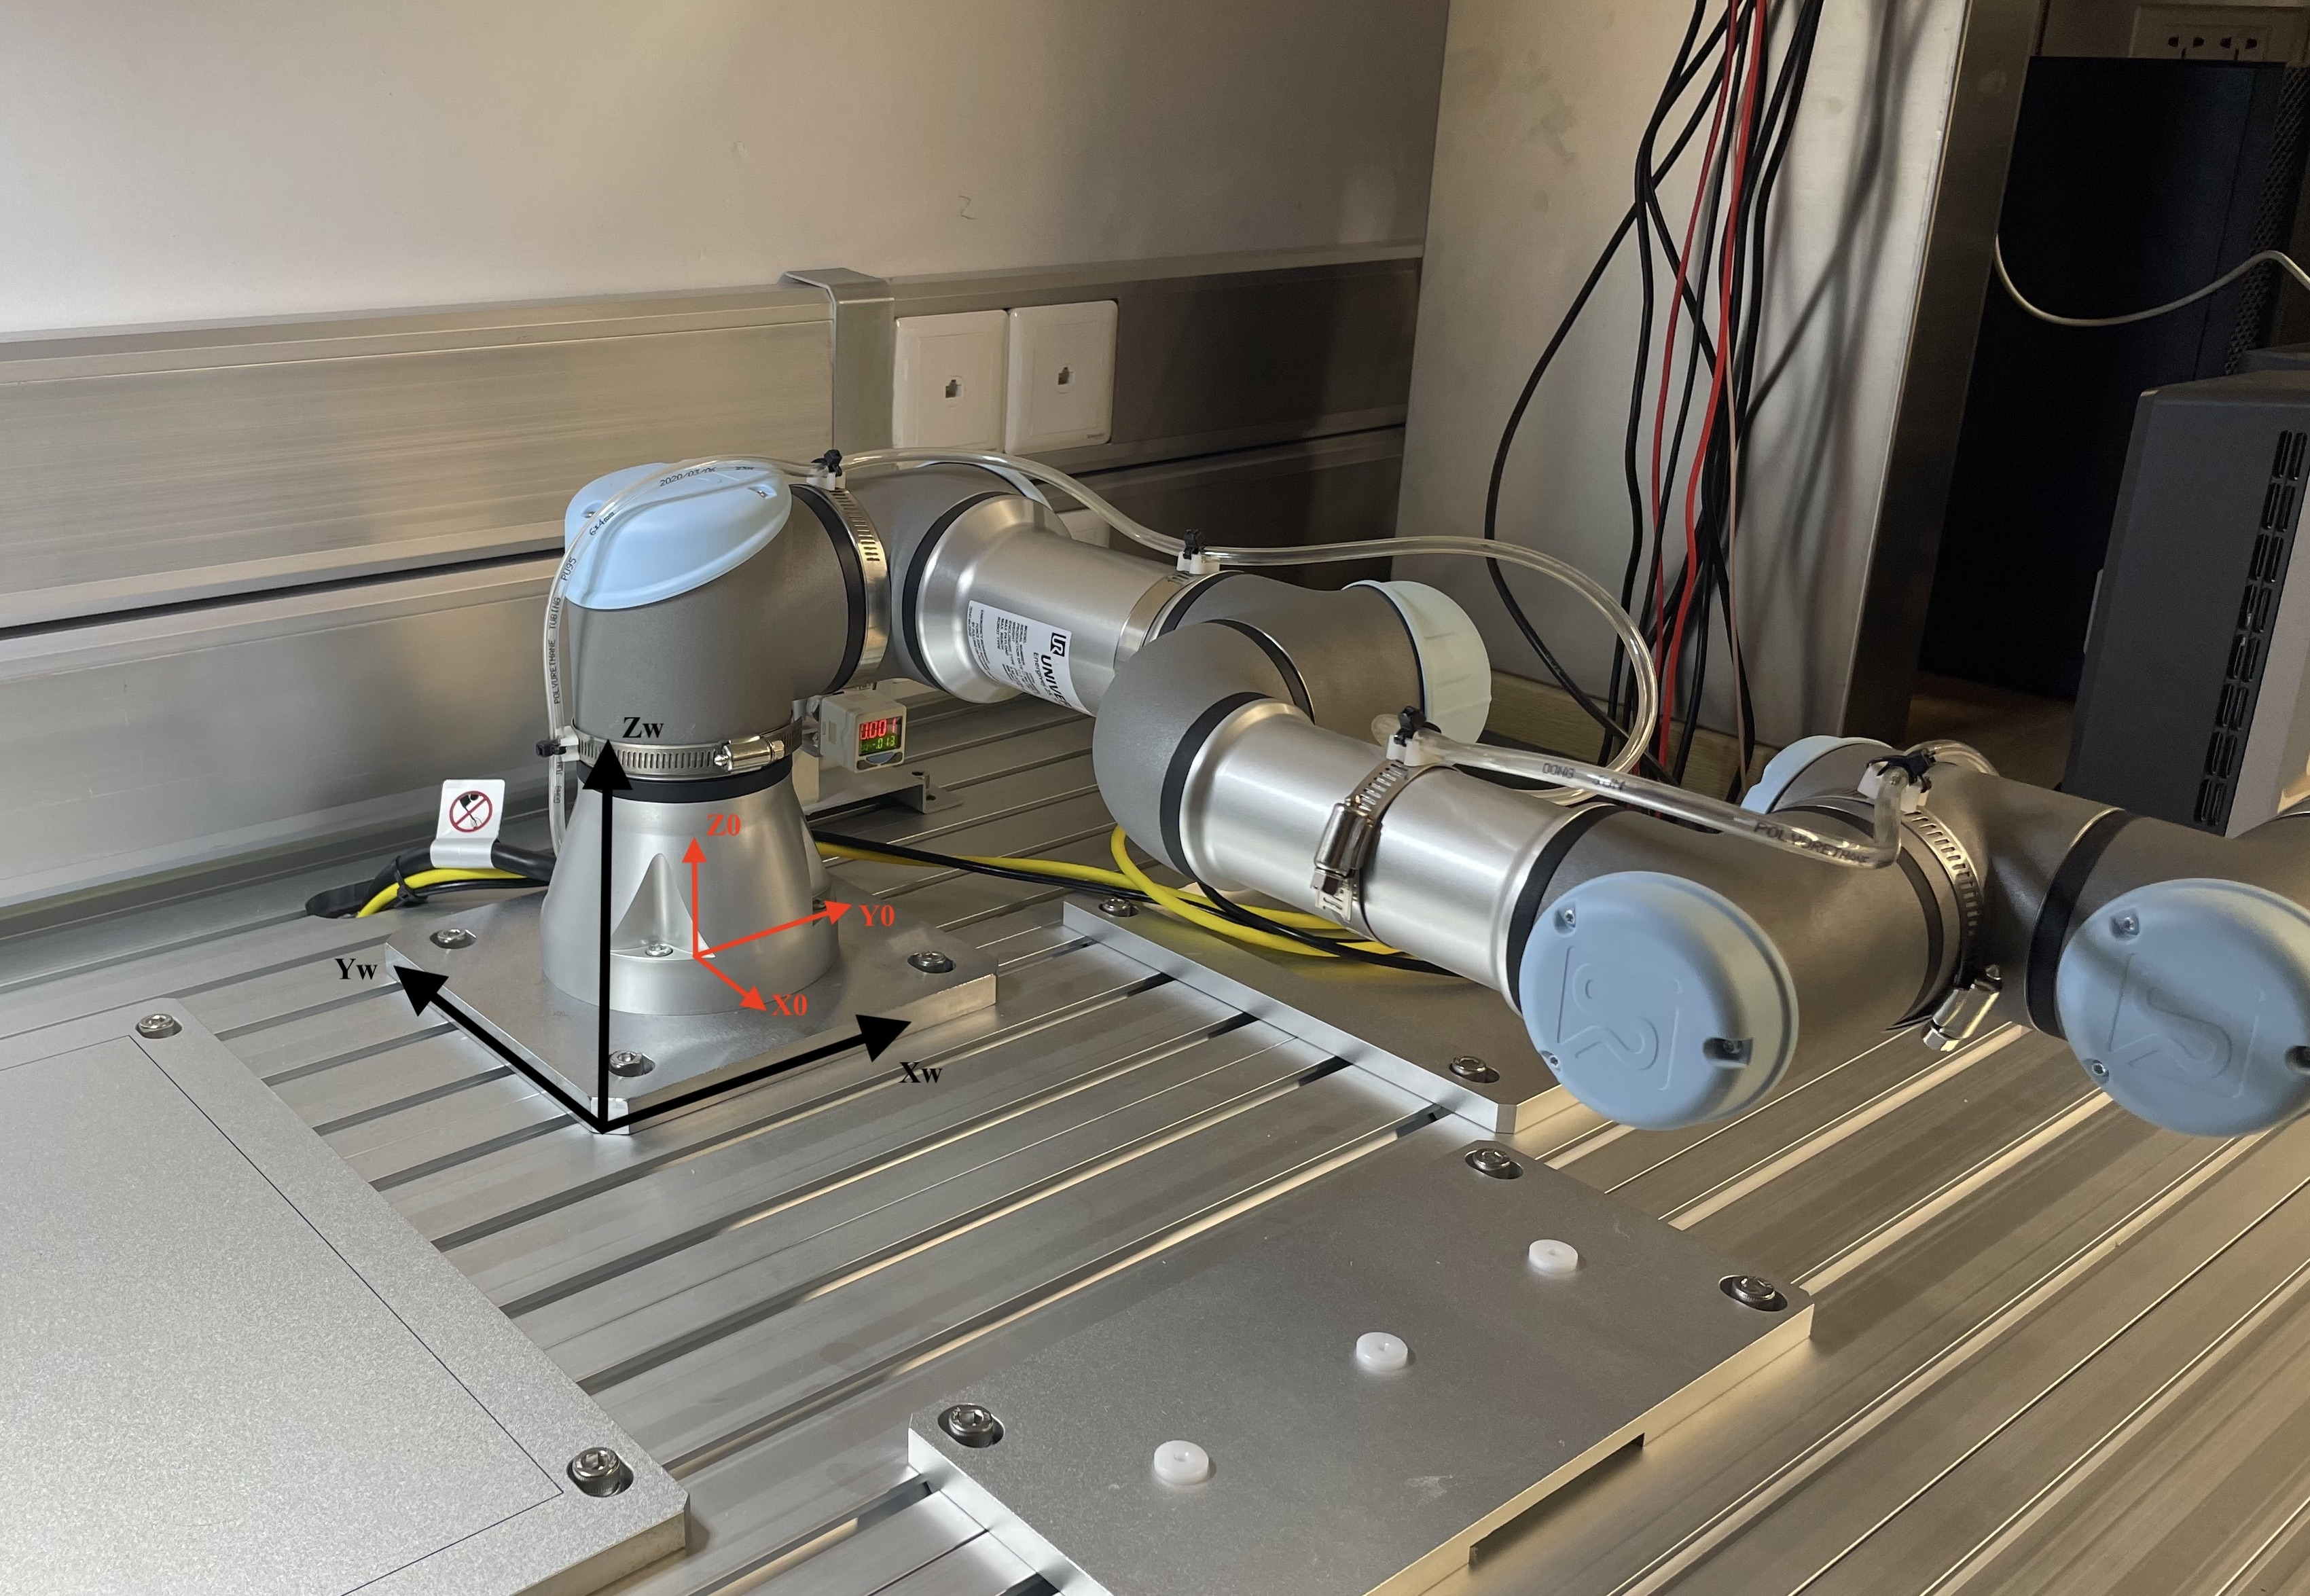
\includegraphics[scale=0.75]{image/lab5_wf0f_1.jpg}
	\caption{\figlbl{frames} Correct location and orientation of the world frame.}
\end{figure}

\item Given the desired position of the gripper $(x_{grip},y_{grip},z_{grip})$ (in the base frame) and the yaw angle, find wrist's center point $(x_{cen},y_{cen},z_{cen})$.
\begin{eqnarray*}
	x_{cen}(x_{grip},y_{grip},z_{grip},yaw) =\\
	y_{cen}(x_{grip},y_{grip},z_{grip},yaw) =\\
	z_{cen}(x_{grip},y_{grip},z_{grip},yaw) = 
\end{eqnarray*}

\item Given the wrist's center point $(x_{cen},y_{cen},z_{cen})$, write an expression for the waist angle $\theta_1$.  Make sure to use the \textbf{atan2()} 
function instead of \textbf{atan()} because \textbf{atan2()} takes care of the four quadrants the x,y coordinates could be in.  
\begin{equation}
	\theta_1(x_{cen},y_{cen},z_{cen}) = 
\end{equation}
\item Solve for the value of $\theta_6$, given yaw and $\theta_1$.
\begin{equation}
	\theta_6(\theta_1,yaw) = 
\end{equation}
\item Find the projected end point $(x_{3end},y_{3end},z_{3end})$ using $(x_{cen},y_{cen},z_{cen})$ and $\theta_1$.  
\begin{eqnarray*}
	x_{3end}(x_{cen},y_{cen},z_{cen},\theta_1) =\\
	y_{3end}(x_{cen},y_{cen},z_{cen},\theta_1) =\\
	z_{3end}(x_{cen},y_{cen},z_{cen},\theta_1) = 
\end{eqnarray*}

\item Write expressions for $\theta_2$, $\theta_3$ and $\theta_4$ in terms of the end point.  You probably will want to define some intermediate
variables to help you with these calculations.
\begin{eqnarray*}
	\theta_2(x_{3end},y_{3end},z_{3end}) =\\
	\theta_3(x_{3end},y_{3end},z_{3end}) =\\
	\theta_4(x_{3end},y_{3end},z_{3end}) = 
\end{eqnarray*}

\item Now that your code solves for all the joint variables (remember that $\theta_5$ is always $-90^{\circ}$) send these six values to the Lab 4 
function \textbf{lab\_fk()}.  You will need to copy you Lab 4 solution into these functions. Do this simply to check that your inverse kinematic calculations are correct. Double check that the x,y,z point that you asked the robot
to go to is the same value displayed by the forward kinematic equations.

\end{enumerate}	
\end{itemize}	

\newpage

\section{Report}
You should submit a lab report using the guidelines given in the ECE 470: How to Write a Lab Report document.  Please be aware of the following:
\begin{itemize}
    \item \textbf{Lab reports are due with your demo for lab 5!}
    \item Lab reports will be submitted online at \href{https://learn.intl.zju.edu.cn/}{Blackboard}.
\end{itemize}
Your lab report should include the following:
\begin{itemize}
% 	\item Coversheet containing your name name, ``Lab 4'', and the weekday and time your lab section meets (for example, ``Tuesday, 3pm'').
    \item A clearly written derivation of the inverse kinematics solution for each joint variable $\left(\theta_{1},\theta_{2},\theta_{3},\theta_{4},\theta_{5},\theta_{6}\right)$. You \textbf{must} include figures in your derivation. Diagrams should be your own creation and clear and easily read.  Do not use hand drawn figures or annotations.
\item For each test point include:
    \begin{itemize}
        \item The given $\{\left(x_{w_{grip}}, y_{w_{grip}},z_{w_{grip}}\right),\theta_{yaw}\}$
        \item The measured position
        \item The scalar error
    \end{itemize}
\item Include a brief discussion of sources of error.

\end{itemize}

As appendices to your report, include the following:
\begin{itemize}
    \item Your $\textbf{lab5\_func.py}$ code and $\textbf{lab5\_exec.py}$ if it was edited.
\end{itemize}

\section{Demo}
Your TA will require you to run your program twice, each time with a different set of desired position and orientation. Your program should reach the desired position and orientation with almost no error. You will be required to be able to demo on the simulator, even if you choose to demo on the real robot.

\section{Grading}
\begin{itemize}
% \item If you don't show up in the in-person and online labs, you \textbf{automatically lose up to 30 points} unless you have a excused absence. Not seeing this line is not a valid one.
% \item 10 points, by the \textbf{end of the first two hour lab session}, show your TA your equations for finding $x_{cen}$, $y_{cen}$, $z_{cen}$.
% \item 10 points, take home assignment after first two hour lab session, by the \textbf{start of the second two hour lab session}, show your TA your equations for $\left\{\theta_1,\theta_2,\theta_3,\theta_4,\theta_5,\theta_6\right\}$.
% \item 10 points, by the \textbf{end of the second two hour lab session}, show your TA your inverse kinematic equations for $\left\{\theta_1,\theta_2,\theta_3,\theta_4,\theta_5,\theta_6\right\}$ implemented in Python code.  
\item 80 points, successful demonstration.
\item 20 points, individual report.  
\end{itemize}


% \section{Tentative Due Dates - Fall 2020}
% The exact date and time will depend on your lab section and can be found on \href{https://learn.intl.zju.edu.cn/}{Blackboard}.
% \subsection{Group A}
% \begin{itemize}
%     \item Demonstration - Week of November 16
%     \item Report - Week of November 16
% \end{itemize}

% \subsection{Group B}
% \begin{itemize}
%     \item Demonstration - Week of November 30
%     \item Report - Week of November 30
% \end{itemize}
%\setcounter{chapter}{4}
\chapter{Robot Vision I: Image Processing}



% \todo[inline]{Edit blob\_search to add more guide comments}
% \todo[inline]{Do we need more HSV guidance?}
% \todo[inline]{Change showmask?}
% \todo[inline]{Make sure we mention circle/keypoints in blob search text}
\section{Important}
Read the entire lab before starting and especially the ``Grading" section so you are aware of all due dates and requirements associated with the lab.  There will be only one online session for this lab, so it is important that you prepare for that one opportunity to work with your TA.

\section{Scope}
\begin{itemize}
    \item Image Representation including Gray-scale image representation, Thresholding and Binarization.
    \item Image Processing including Filtering, Connectivity and Edge detection
    \item Image Analysis including Object segmentation, Pose estimation and Classification
\end{itemize}    

\section{Objectives}

This is the capstone lab of the semester and will integrate your work done in previous labs with python, ROS, and forward and inverse kinematics.  It will also introduce you to some basic OpenCV techniques.  In this lab you will:
\begin{itemize}
	\item Use OpenCV functions to distinguish the shape of the blocks and find the centroid and angle of them.
	\item Develop transformation equations that relate pixels in the image to coordinates in the world frame
	\item Report the world frame coordinates $(x_w,y_w)$ of the centroid of each block in the camera’s view.
	\item Move the block to a predefined position in the robot's work area.
\end{itemize}


\section{Background}

\begin{itemize}
	% \item Appendix \ref{computervision} which explains how to derive the intrinsic and extrinsic equations for the camera.
    % \item HSV Color Space:
    % \begin{itemize}
    % \item \url{https://en.wikipedia.org/wiki/HSL_and_HSV}
    % \item \href{https://stackoverflow.com/questions/10948589/choosing-the-correct-upper-and-lower-hsv-boundaries-for-color-detection-withcv}{https://stackoverflow.com/questions/10948589/}
    % \item \href{https://www.rapidtables.com/convert/color/rgb-to-hsv.html}{Converting RGB to HSV}
    % \end{itemize}
    
    % \item Simple Blob detector:
    % \begin{itemize}
    % \item \url{www.learnopencv.com/blob-detection-using-opencv-python-c/}
    % \item \href{https://stackoverflow.com/questions/8076889/how-to-use-opencv-simpleblobdetector}{https://stackoverflow.com/questions/8076889/}
    % \item \url{https://www.programcreek.com/python/example/89350/cv2.SimpleBlobDetector}
    % \item \url{https://www.programcreek.com/python/example/71388/cv2.SimpleBlobDetector_Params}
    % \end{itemize}
    \item Image Acquisition \\
Image sensors, like many other types of sensors, acquire signal from the surrounding to
obtain information pertaining to the environment. Signals can be generated from light wave,
or other form of energy for example (acoustic in ultrasound imaging) by an imaging system.
The process of acquiring images of the surrounding scene is an important aspect for robot
applications. As robots are usually expected to accomplish specific tasks while interacting with
the environment, a typical robot vision system involves processing video stream on-the-fly
for timely feedback control or decision making. Hence, connecting imaging systems to the
robot becomes an important aspect for robot vision.

A camera device is often used to acquire timely visual information of the surrounding. In
this lab, we will connect a camera to capture images represented as digital information for
processing and computational operation.
\end{itemize}



\begin{itemize}
    \item Image Processing \\
Behind the scenes of robot vision lies image processing operations that enhance, analyze
and/or transform the image data. In robot vision, a robot makes sense of the surrounding
through acquired and processed images that present useful information including colors,
geometries, structures and motions.

In this lab, we process images by applying thresholding, binarization and filtering. Image
analysis is performed through edge detection, object segmentation, pose estimation and
similarity score measurement.
\end{itemize}   


\section{Tasks}
In this lab, we will be using some built in functions in the \textbf{OpenCV} library to locate blocks based on their shape and find their centroids.  \textbf{OpenCV} is a powerful set of open source tools that are useful for computer vision tasks.  They will allow us to efficiently complete tasks without having to develop the algorithms ourselves.

% \subsection{Description}
In this lab, we have several randomly placed blocks with different shapes and directions under an industrial camera, as is showed in the \figref{lab5description}.
All we need to do is to stack the block of the \textbf{same shape} in the \textbf{same direction} together.
The destination is not specified. Any place in the upper right area is fine. 

\begin{figure}
	\centering
		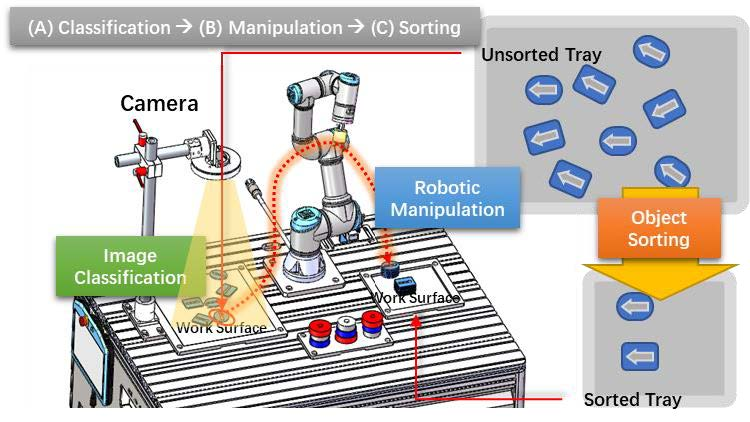
\includegraphics[scale=0.9]{image/lab6_table.jpg}
	\caption{\figlbl{lab5work} Task Description including Image Classification, Robot Manipulation and Object Sorting}
\end{figure}

\begin{figure}
	\centering
		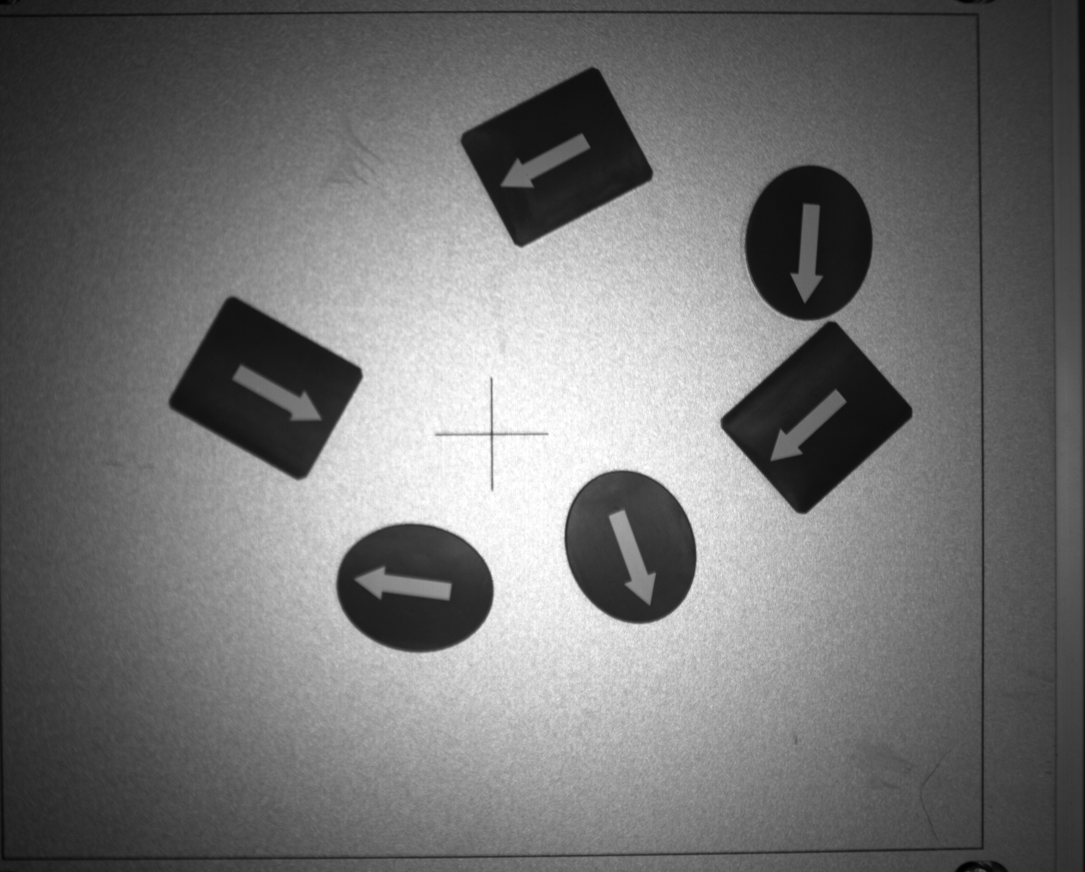
\includegraphics[scale=0.2]{image/lab6_real_pic.jpg}
	\caption{\figlbl{lab5description} Example of randomly placed blocks}
\end{figure}

\begin{figure}
	\centering
		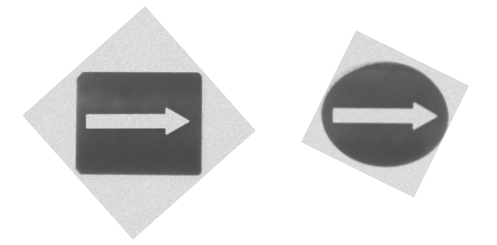
\includegraphics[scale=0.5]{image/lab6_example.jpg}
	\caption{\figlbl{lab5example} example.jpg}
\end{figure}

% Thresholding is the way we will isolate the objects that we are interested in by color.  We will be using the HSV color space to accomplish this.  HSV stands for Hue, Saturation and Value.  Using \textbf{OpenCV}, we will mask out any objects that don't fall within the desired HSV range that we set.  This allows us to focus only on the green and yellow blocks that we wish to locate.


% \textbf{Side Note:}  What is the H,S,V color space?  Please see the reference link to the Wikipedia  page discussing color spaces.  You are probably most familiar with the R,G,B (red,green,blue) color space.  Here each pixel of an image has a R,G,B value.  With H,S,V colors are placed on a color wheel and you indicate which color you are interested in by selecting an angle range.  In \textbf{OpenCV} the range of the angle is from 0 degrees to 180 degrees.  (You will find other implementations that use 0-360).  For example a blueish color would be in the angle range of 110 degrees to 130 degrees.  The S value is a number between 0 and 255 with 0 being very white and washed out and 255 the full, clear color.  The V value is also a number between 0 and 255 with 0 being very dark and shaded and 255 the full clear color.  The main reason we use the H,S,V color space in this lab is that it makes finding a color with different shading and lighting conditions much easier. 

% Once we have thresholded the image, we are left with `blobs'.  Blobs consist of the groups of pixels that were not masked out by thresholding.  No matter how well we perform thresholding, there will always be noise in the image.  We only really care about the blobs that correspond to the blocks we wish to find and the \textbf{OpenCV} function \textbf{SimpleBlobDectector} can help us do that.  It allows us to filter out blobs based on features like size, roundness, eccentricity, etc.  In addition, once we have narrowed down to the blobs we care about, it can help us find the centroid of these blobs.


% \subsection{Camera Calibration and Transformation}
% The problem of camera setup is that of relating (row,column) coordinates in an image to the corresponding coordinates in the world frame $(x_w,y_w,z_w)$.  A camera transformation equation will be developed to allow us to perform this conversion. Several parameters must be specified in order to implement the equations. Specifically, we are interested in \textbf{$\theta$} the rotation between the world frame and the camera frame and \textbf{$\beta$} the scaling constant between distances in the world frame and distances in the image and $T_{x}$ and $T_{y}$ the relationship between the origin of the camera frame and the world frame. Due to simulation limitations, these values and others have been provided for you.

% Appendix \ref{computervision} will guide you through the development of the camera transformation equations and explain the camera calibration process.

% \subsection{Pick and Place}
% Your program should:

% \begin{itemize}
% \item Move the Robot out of the way so that the camera can view the entire work area in order to find the blocks randomly placed in that area.  

% \item Use \textbf{OpenCV} functions to find the centroid $(x_w,y_w)$ of each block.

% \item Display a center point and a circle around each discovered block in the video display window.  

% \item Command the robot to pick up each block one at a time and place it in the appropriate goal position. 

% \item When finished with all blocks exit from the program.  

% \end{itemize}

\section{Procedure}
\subsection{Lab Set Up}
Start as you normally do by downloading the Lab 5 starter files from the lab website, unzip them and place them in your \textbf{src} directory along with the rest of the lab packages.

If you look inside \textbf{lab5pkg\_py/scripts}, you will see a number of Python files, but we will only be editing a few during this lab.  A brief description of each file is provided here:
\begin{itemize}
    \item \textbf{lab5\_exec.py} - The main executable.  It contains all the code to move the arm.  You will edit this to complete the pick and place task.
    % \item \textbf{lab5\_blob\_search.py} - This contains all the code related to image thresholding and finding blobs and centroids.  You will edit this to locate the desired objects and return their positions in pixel coordinates.
    % \item \textbf{lab5\_coordinate\_converter.py} - This contains the camera calibration and transformation code. You will edit this to add in the camera transformation equations.
    \item \textbf{lab5\_func.py} - This contains the forward and inverse kinematics code.  You should edit to add your solutions from Lab 3 and 4.
    \item \textbf{lab5\_header.py} - This is a standard header file with imports and constant definitions.  There is no need to edit this.
    % \item \textbf{lab5\_gen\_image.py} and \textbf{lab5\_spawn\_block.py} - These are used to generate blocks to pick up.  Do not edit.
    \item \textbf{lab5\_img.py} - This contains all the image processing, camera calibration and transformation code. You will edit this to process your image, find the camera transformation equation.
    \item \textbf{CMakeLists.txt} a file that sets up the necessary libraries and environment for compiling lab5\_exec.py.
    \item \textbf{package.xml} This file defines properties about the package including package dependencies.
    \item \textbf{README} To run lab5 code on real robot, please read it \textbf{FIRST}!
    \item Every time you open a new terminal, you need to run \textbf{source devel/setup.bash} in your catkin folder.
    
\end{itemize}

\subsection{Image Acquisition}
In this lab, we just capture the image manually. First, copy the folder \textbf{Snapshot} in folder \textbf{lab5pkg} to the \textbf{Windows} System.
Then you can edit the python script \textbf{save\_image.py} to change the directory where your snapshots will save
before you run it to store a series of images. After that, we can use these images in our ROS programming.

\subsection{Image Processing}

In order to distinguish the shape of the blocks, we use a template matching method here. 
The \textbf{example.jpg} ,shown in \figref{lab5example},is the given template, including a rectangular block and an elliptical one.
Then the similarity measurement of the target block can help with the classification problem when comparing with the template.

{\footnotesize
%\tiny{
%\begin{verbatim}[obeytabs,tabsize=4]
%\footnotesize{
\begin{verbatim}
    rospack = rospkg.RosPack()
    lab5_path = rospack.get_path('lab5pkg_py')
    img_path = os.path.join(lab5_path, 'scripts', 'example.jpg')
    _img = cv2.imread(img_path)
    _draw_img = _img.copy()

    _blur = cv2.bilateralFilter(_img, 19, 130, 30)
    _blur = cv2.medianBlur(_blur, 9)

    _img_gray = cv2.cvtColor(_blur, cv2.COLOR_BGR2GRAY)
    _xgrd = cv2.Sobel(_img_gray, cv2.CV_16SC1, 1, 0)
    _ygrd = cv2.Sobel(_img_gray, cv2.CV_16SC1, 0, 1)
    _img = cv2.Canny(_xgrd, _ygrd, 30, 220)
\end{verbatim}}
Code Explanation: First, we obtain the path to the template \textbf{example.jpg} and read it subsequently by the \textbf{OpenCV} method \textbf{cv2.imread}.
Then we preprocess the image by \textbf{cv2.bilateralFilter} and \textbf{cv2.medianBlur}.
Bilateral filter can smooth images while preserving edges by means of a nonlinear combination of nearby image values.
And median filter is also common to eliminate isolated noise.
After converting image to gray-scale using \textbf{cv2.cvtColor}, we can exploit \textbf{Sobel} and \textbf{Canny} operator
to detect the edge of the template.

\begin{figure}
	\centering
		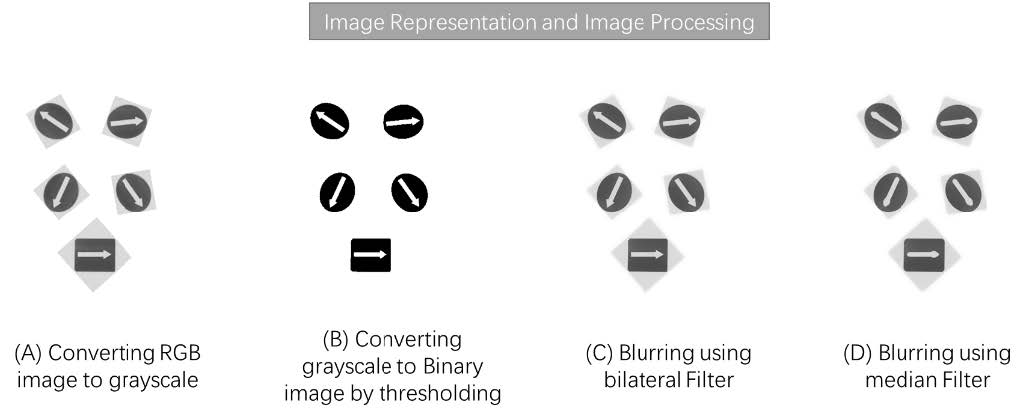
\includegraphics[scale=1]{image/lab6_img_process.jpg}
	\caption{\figlbl{lab5_1} Image Representation and Image Processing}
\end{figure}

\begin{figure}
	\centering
		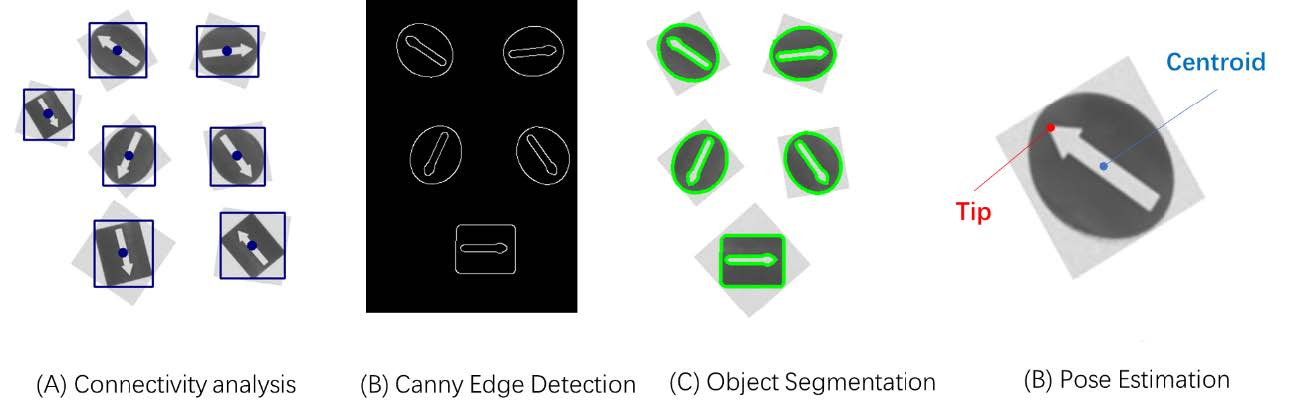
\includegraphics[scale=0.9]{image/lab6_edge.jpg}
	\caption{\figlbl{lab5_2} Image Representation and Image Processing}
\end{figure}

{\footnotesize
%\tiny{
%\begin{verbatim}[obeytabs,tabsize=4]
%\footnotesize{
\begin{verbatim}
    _w, _h = _img.shape
    # rectangle
    _img_1 = _img[:, :_w]
    # ellipse
    _img_2 = _img[:, _w:]

    # rectangle
    _img_1, _contours_1, hierarchy = cv2.findContours(_img_1, cv2.RETR_TREE, cv2.CHAIN_APPROX_SIMPLE)
    # ellipse
    _img_2, _contours_2, hierarchy = cv2.findContours(_img_2, cv2.RETR_TREE, cv2.CHAIN_APPROX_SIMPLE)
\end{verbatim}}

Code Explanation: Here we divide the image into two parts, i.e., rectangle and ellipse.
Then we use \textbf{cv2.findContours} to find contours. Variables \textbf{\_contours\_1} and \textbf{\_contours\_2} store all contours, each of which is composed of
a series of pixel points.\\
\textbf{IMPORTANT}: Before you use the contours found by \textbf{cv2.findContours}, please check and ensure these are what you want!
And Try to figure out why the number of contours is twice.

{\footnotesize
%\tiny{
%\begin{verbatim}[obeytabs,tabsize=4]
%\footnotesize{
\begin{verbatim}
    # compute the center of a contour
    N = cv2.moments(contours[i * 2])
    _center_x = int(N["m10"] / N["m00"])
    _center_y = int(N["m01"] / N["m00"])
    # draw a circle on the center point
    cv2.circle(draw_img, (int(_center_x), int(_center_y)), 7, [0,255,0], -1)
\end{verbatim}}

Code Explanation: Here we use \textbf{cv2.moments} to compute the centroids and label a circle on the center point
by \textbf{cv2.circle}.


% \subsection{Running the Program}
% To run the code, open a terminal window and in your catkin working directory:
	
% % \begin{lstlisting}[language=bash]
% %     $ source devel/setup.bash
% %     $ roslaunch lab5pkg_py lab5.launch
% % \end{lstlisting}
% \begin{lstlisting}[language=bash]
%     $ source devel/setup.bash
%     $ roslaunch ur3_driver ur3_gazebo.launch
% \end{lstlisting}

% Then open a second terminal window and in your catkin working directory:
    
% \begin{lstlisting}[language=bash]
%     $ source devel/setup.bash
%     $ rosrun lab5pkg_py lab5_coordinate_converter.py
% \end{lstlisting}

% Then open a third terminal window and in your catkin working directory:
    
% \begin{lstlisting}[language=bash]
%     $ source devel/setup.bash
%     $ rosrun lab5pkg_py lab5_exec.py --missing False 
%     --image 0
% \end{lstlisting}


% The -{}-\textit{missing} flag, when \textbf{True}, will allow you to test your gripper feedback implementation.  The -{}-\textit{image} flag will change what image is being displayed.  It is normally set to image 0, but can be changed so you can test all 5 images i.e 0 to 4.  Each image represents a different set of block locations.  Your final code must work on all five images. The code has been divided up like this to aid you in working with it.  You should not need to restart Gazebo while making edits to files, but you can easily restart the coordinate converter node after you edit that file.  The executable will naturally stop after completing its tasks.

% When you run the program, you will see two image windows pop-up.  One is the color or raw image.  The other is a black and while masked image that will change based on your threshold values.  Note that sometimes the two windows will appear on top of each other making it appear that one is not present.  Simply move the top window to see both.



% \subsection{Threshold camera image to distinguish the colors of choice} \label{ObjCentriod}
% In \textbf{lab5\_blob\_search.py}, in the function \textbf{blob\_search(...)}, you will edit the following to locate the green and yellow blocks.  They are currently set to threshold blue colored objects.
% {\footnotesize
% \begin{verbatim}
%     lower = (110, 50, 50)   # Blue lower
%     upper = (130, 255, 255) # Blue upper
% \end{verbatim}}

% Selecting the correct values for thresholding can be rather challenging and requires some trial and error.  There are several methods that you can use to find these values.  One is to review how the HSV color space works and select an appropriate Hue value.  Once that is selected, you should adjust Saturation and Value until a clean image is created.  If necessary, you may need to widen or narrow your Hue range.  Another method is to convert the RGB value given in the image window to an HSV value.  Note the RGB values displayed in the lower left hand corner of \figref{centroid}.  They represent the RGB value of what ever pixel the mouse pointer is hovering over.  Using these values in a website like the one listed in the references will allow you to get a starting point for your HSV ranges.  Pay attention to how the HSV value is represented on the website compared to the way it is represented in \textbf{OpenCV}. Note that you will have to create a different set of ranges for for each color and select the appropriate range depending on what color you are looking for.

% When successfully completed, you will see a black and white image with white shaped blobs that have little `noise' inside their boundaries.  It is okay to have more than one blob in the image as long the block we desire is seen as this process works in conjunction with blob detection to isolate the desired block.  See \figref{thresh} for reference. You will only see one threshold image at a time.  When you you are done viewing the image, you should press the enter key to move to the next step - make sure the image window is selected when you hit enter and not a terminal or other window.
% \begin{figure}[ht]
% \centering
% 	
\includegraphics[height=6cm]{lab5_threshold.png}
% \caption{\figlbl{thresh} A well thresholded image.  Note you can see the block clearly.}
% \end{figure}


% \subsection{Blob Detection}
% In \textbf{lab5\_blob\_search.py}, in the function \textbf{blob\_search(...)}, you will edit the following to identify blobs within the thresholded image.
% {\footnotesize
% \begin{verbatim}
%     # Setup SimpleBlobDetector parameters.
%     params = cv2.SimpleBlobDetector_Params()

%     # Filter by Color
%     params.filterByColor = False

%     # Filter by Area.
%     params.filterByArea = False

%     # Filter by Circularity
%     params.filterByCircularity = False

%     # Filter by Inertia
%     params.filterByInertia = False

%     # Filter by Convexity
%     params.filterByConvexity = False
% \end{verbatim}}
% Currently all the `filterBy...' parameters are set to False.  You need to decide which filter parameters you want to use to limit the detected blobs to the block you care about.  This is done by setting it to \textbf{True} and adding the necessary parameters to the code.  You should consult the \textbf{OpenCV} references for help in understanding what these parameters mean and how to properly set them.  It is not necessary or desirable to use all the parameters, so you only need to select the ones that you think will help. When set correctly, the only keypoints detected will be those of the desired block and their centroids will be drawn accurately on the block as seen in \figref{centroid}. Note that these parameters will have no effect on the mask view, only the keypoints found.  In order to mark the keypoints and draw a circle around the block, complete the following code and uncomment them:
% {\footnotesize
% \begin{verbatim}
%     # Draw a circle around the detected block
%     # im_with_keypoints = cv2.circle(image_raw, (int(c), int(r)), ???)

%     # Draw the keypoints on the detected block
%     # im_with_keypoints = cv2.drawKeypoints(im_with_keypoints, keypoints, ???)


% \end{verbatim}}

% \begin{figure}[ht]
% \centering
% 	
\includegraphics[height=6cm]{lab5_centroid.png}
% \caption{\figlbl{centroid} A properly drawn centroid on the block.}
% \end{figure}



% \subsubsection{Camera Calibration}
% Camera calibration is the process of figuring out the parameters used in the camera transformation. \textbf{lab5\_coordinate\_converter.py} contains these values.
% {\footnotesize
% \begin{verbatim}
%     # Params for camera calibration
%     theta = -0.09
%     beta = 730.0
%     tx = -0.297435628054
%     ty = -0.0763807206584
% \end{verbatim}}


% \subsubsection{Camera Transformation}
% Camera transformation will be completed in in \textbf{lab5\_coordinate\_converter.py}.  You should work through the process of finding the camera transformation equations in Appendix \ref{computervision}.  These equations will then be entered into the function \textbf{IMG2W(r,c)}.  The goal of this function is to take the received pixel values and convert them to world frame coordinates in meters.  When you update this file, you need to restart the coordinate converter node for the changes to take effect.

% \subsection{Pick and Place}
% To complete the pick and place portion of this lab, you will need to edit \textbf{lab5\_exec.py}.  There are a number of tasks in this section that should be familiar to you from Lab 2.  
% In the \textbf{main()} function, you will have to complete the logic of the pick and place task. 


% {\footnotesize
% \begin{verbatim}
%     # Call blob search
%     green_image_rc = blob_search(cv_image.copy(), 'green')
%     yellow_image_rc = blob_search(cv_image.copy(), 'yellow')
% \end{verbatim}}

% After calling \textbf{blob\_search(...)}, you will have the location of the green and yellow blocks in pixels.  You will then need to pass this data to \textbf{lab5\_coordinate\_converter.py} so we can get the position in world coordinates.  To do this, we will create a publisher to pass the pixel values to our coordinate converter.  Then, when it is done converting the image, we will subscribe to the coordinate converter's output.  Note that a small break between the publishing the data to the image coordinate converter and making use of the subscriber's output maybe needed to prevent accessing old data (Suggestion: Look at \textbf{rospy.sleep(...)}).  The publisher and subscriber will use the \textbf{Point} message type and you should research this to figure out what data it contains.

% You will also need to complete the \textbf{move\_block(...)} function.  While this is similar to the work done in Lab 2, we now no longer have hard coded angle values.  You will need to use your inverse kinematics to find these angles.  The goal positions are provided in the code.  Additionally, your \textbf{move\_block(...)} function should detect missing blocks as you did in Lab 2.  If a missing block is found the program should move the arm back to home and halt the program with an error message.

% When complete, you will be able to run the code on any of the five images and it will locate, pick up and place both colored blocks.

\subsection{Debugging}
This lab can be a bit tricky to work through as several parts require trial and error.  Here are some suggestions:
\begin{itemize}
    \item Approach the lab sequentially and make sure you get good results at each step.
    \item Comment out parts that you are not currently using (Don't forget the uncomment them though...)
\end{itemize}


\section{Report}
This lab does not require a formal lab report - only the submission of your code.  You should a submit a document to \href{https://learn.intl.zju.edu.cn/}{Blackboard} containing all of the files that you edited to complete the lab.  This will be submitted to \href{https://learn.intl.zju.edu.cn/}{Blackboard} as in the past.

\section{Demo}
Your TA will require you to run your program twice, each time with different initial block positions and verify that your program can locate the blocks and place them in the correct location.  You will also demonstrate that suction feedback is working.

\section{Grading}
\begin{itemize}
\item 100 points, successful demonstration and submission of the code. (No code = 0 points)
\end{itemize}


% \section{Tentative Due Dates - Fall 2020}
% Lab 5 demonstration will be due by 5PM on Wednesday, December 16.  Code must be submitted on \href{www.gradescope.com}{GradeScope}, by midnight that same day.  Note that each TA will only have a limited number of office hours prior to this time, so you should plan ahead to meet this deadline.


\chapter{Robot Vision II: Camera Calibration}



\section{Important}
Read the entire lab before starting and especially the ``Grading" section so you are aware of all due dates and requirements associated with the lab.  There will be only one online session for this lab, so it is important that you prepare for that one opportunity to work with your TA.

\section{Scope}
\begin{itemize}
    \item Camera Calibration - Obtain the relation between camera and world reference frame
    \item Robot-Camera Calibration - Obtain the mapping between the camera and robot coordinates
    \item Image-Guided Manipulation - Plan and execute path for manipulation task
\end{itemize}    

\section{Objectives}

This is the capstone lab of the semester and will integrate your work done in previous labs with python, ROS, and forward and inverse kinematics.  It will also introduce you to some basic OpenCV techniques.  In this lab you will:
\begin{itemize}
	\item Use OpenCV functions to distinguish the shape of the blocks and find the centroid and angle of them.
	\item Develop transformation equations that relate pixels in the image to coordinates in the world frame
	\item Report the world frame coordinates $(x_w,y_w)$ of the centroid of each block in the camera’s view.
	\item Move the block to a predefined position in the robot's work area.
\end{itemize}


\section{Background}
\subsection{The Camera Model and Calibration Process}
    Robotic systems commonly rely on visual information from the surrounding to perceive
the environment. The source of this information typically comes in the form of images
depicting the scene of the camera views. Therefore, camera can be an extremely useful
sensing device to provide a robotic system with control feedback and perception. Like many
other sensors, there is usually a need to map the acquired signal (imagery) to measurement
(spatial) through a calibration process based on a camera model. The central projection
camera model as shown in \figref{lab6model} is a representation of the image formation process relating
points in world coordinates to their projection on a virtual image plane.
\begin{figure}
	\centering
		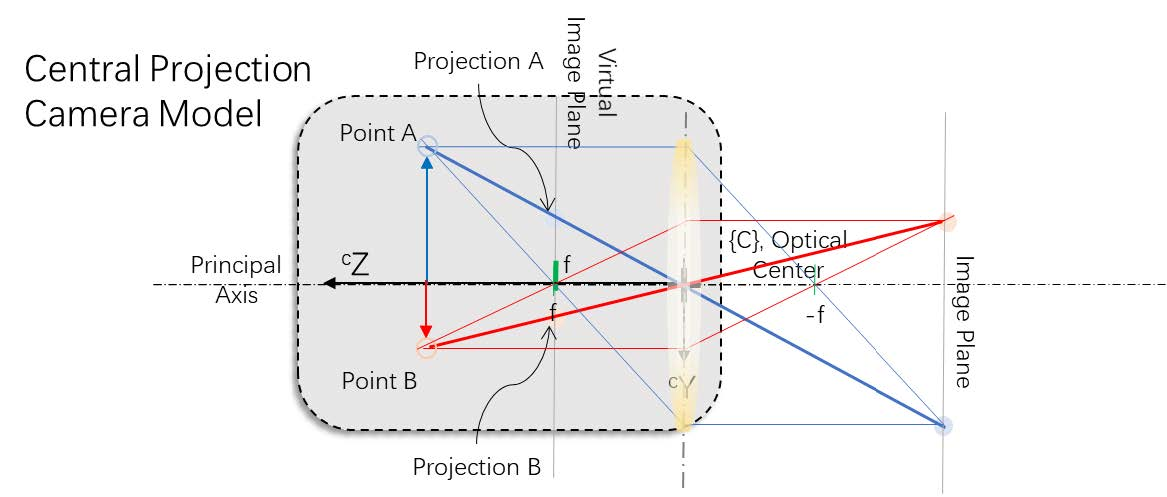
\includegraphics[scale=1]{image/lab7_camera.jpg}
	\caption{\figlbl{lab6model} Central Projection Camera Model}
\end{figure}

Camera calibration uses known image data of scene from different camera views to
establish a mapping between the camera pose and the world reference. This mapping is
usually in the form of a camera calibration matrix expressed as
\begin{equation}
    M=C(R \mid t)
\end{equation}
where $R$ and $t$ are the 3-by-3 rotation matrix and 3-by-1 translation vector, respectively, from 
the camera's viewpoint. Together they are known as the extrinsic matrix. Matrix $C$ is a 3-by-3 matrix
with intrinsic parameters including its focal length $(f_x,f_y)^T$, principal point $(i_c,j_c)^T$
expressed as
\begin{equation}
    \mathbf{C}=\left(\begin{array}{ccc}
    f_{x} & a & i_{o} \\
    0 & f_{y} & j_{o} \\
    0 & 0 & 1
    \end{array}\right)
\end{equation}
Lens distortion model is often included to account for the distorting effect with the lens.
The warping effect can be modeled using Brown-Conrady model in which a distorted pixel
can be compactly expressed as
\begin{equation}
    \overline{\mathbf{X}}_{\text {distort }}=\left(1+k_{1} r^{2}+k_{2} r^{4}\right)\left(\begin{array}{l}
    \bar{x} \\
    \bar{y}
    \end{array}\right)+\left(\begin{array}{ll}
    l_{1} & l_{2}
    \end{array}\right)\left(\begin{array}{cc}
    2 \overline{x y} & r^{2}+2 \bar{y}^{2} \\
    r^{2}+2 \bar{x}^{2} & 2 \overline{x y}
    \end{array}\right)
\end{equation}

where $\left(\begin{array}{ll}\bar{x} & \bar{y}\end{array}\right)^{\mathrm{T}}$ is the normalized image projection $\mathrm{C}\left(\begin{array}{ll}x / z & y / z\end{array}\right)^{\mathrm{T}}$
,and $r$ represents norm $\left(\left(\begin{array}{ll}\bar{x} & \bar{y}\end{array}\right)^{\mathrm{T}}\right)$.
The radial and tangential distortion coefficients are denoted by $k_{1-2}$ and $l_{1-2}$,respectively.
In this lab, we will use a simplified model where the imaging plane is parallel to the work
surface. Hence, relation between the image coordinates and world reference frame reduces
to 1-dof rotation and 2-dof translation and scaling. Since the 2-dof scaling can be
determined independently based on the parallel constraint, the camera calibration process
reduces to obtaining the orientation and translation of the work surface and imaging plane.



\subsection{The Robot-Camera Calibration Process}
In order to guide robot manipulation using images acquired from the camera, we need
to first know the spatial relationship between the camera and the robot. Combining with the
camera calibration matrix, we will be able to, under the appropriate specified constraints, map
image coordinates to robotic joint coordinates for path planning and execution to accomplish
manipulation tasks. There are many robot-camera calibration approaches for different
conditions and application.

To simplify the demonstration of robot-camera calibration process, this lab will use an
eye-to-hand model, where the camera is fixed with respect to the world coordinate system
with known spatial relationship to the robot base. Combing the camera calibration model, we
can now map image coordinates to world coordinates referenced from the base and
subsequently the robotic joint coordinates.


\section{Lab Activities}
In this lab we will use the image processing techniques demonstrated in previous lab to detect,
and label objects in the camera scene hence guiding manipulation tasks in object classification
and sorting as illustrated below.

\begin{figure}
	\centering
		
\includegraphics[scale=1]{image/lab7_workflow.jpg}
	\caption{\figlbl{lab6workflow} Workflow for the task of image-guided robotic object sorting}
\end{figure}

\begin{figure}
	\centering
		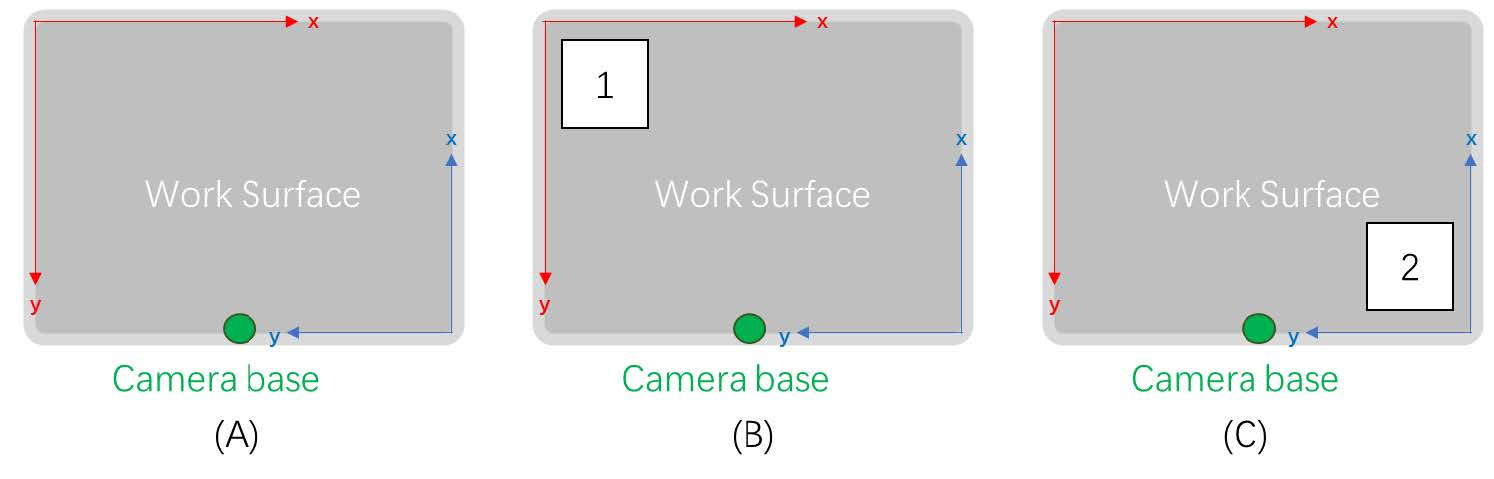
\includegraphics[scale=0.8]{image/lab7_register.jpg}
	\caption{\figlbl{lab6register} Registering two positions to find image-robot relationship}
\end{figure}

\begin{itemize}
    \item Transform Image (Pixel) Coordinates to Robotic Reference Frame
    \begin{itemize}
        \item Define relationship between the robot base frame and the pixel coordinate frame as
        illustrated by the red and blue axes, respectively.
        \item Move robot to Region 1: pixel coordinates $(x_1,y_1)$; register the robot coordinates as $(x_1',y_1')$.
        \item Move robot to Region 2: pixel coordinates $(x_2,y_2)$; register the robot coordinates as $(x_2',y_2')$
        \item Obtain the ratio that map $(x,y)$ to $(x',y')$ as define below:
        \begin{equation}
            \begin{aligned}
            &x_{ratio}=\left(x_{2}^{\prime}-x_{1}^{\prime}\right) /\left(y_{2}-y_{1}\right) \\
            &y_{ratio}=\left(y_{2}^{\prime}-y_{1}^{\prime}\right) /\left(x_{2}-x_{1}\right)
            \end{aligned}
        \end{equation}
        \begin{equation}
            \begin{aligned}
            &x^{\prime}=x^{\prime}_1+x_{ratio} *\left(y-y_{1}\right) \\
            &y^{\prime}=y^{\prime}_1+y_{ratio} *\left(x-x_{1}\right)
            \end{aligned}
        \end{equation}
    \end{itemize}
    \item Classify Objects and Compute Pose (Lab 5: Image Processing)
    \begin{itemize}
        \item Label the objects and
        \item Compute their center positions and orientation in the scene
    \end{itemize}
    \begin{figure}
        \centering
            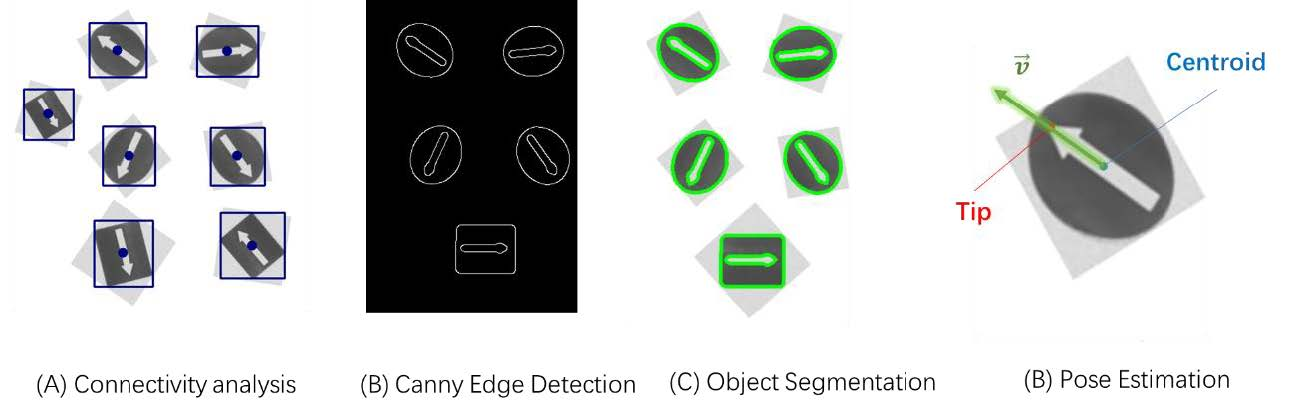
\includegraphics[scale=1]{image/lab7_pose.jpg}
        \caption{\figlbl{lab6process} Image processing to classify and localize object in camera scene}
    \end{figure}

    \item Move Robot using on Transformed Coordinates
    Move robot arm from one position to another as you have done in Lab 4 (inverse kinematics)
    with the Transformed Coordinates,
    \begin{itemize}
        \item Locate objects and check their label as in the image
        \item Transform coordinates to robot coordinate system
        \item Move to pick (suction grip) object from the unsorted tray as should in \figref{lab6flow}
        \item Move to sort objects into specific pose in the sorted tray as shown in \figref{lab6flow}
    \end{itemize}
\end{itemize}

\begin{figure}
	\centering
		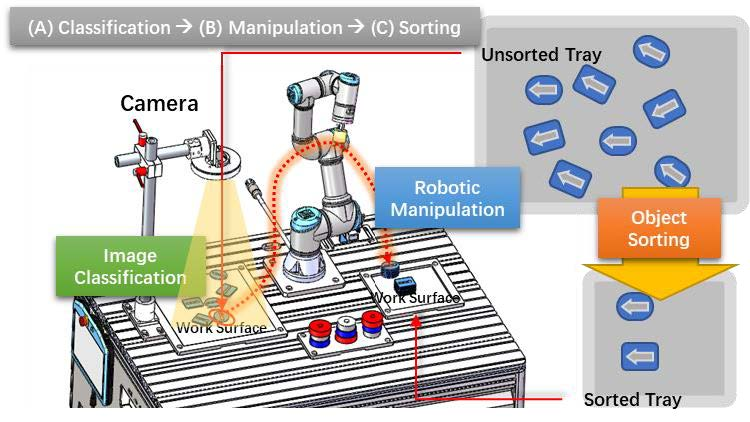
\includegraphics[scale=1]{image/lab6_table.jpg}
	\caption{\figlbl{lab6flow} Image processing to classify and localize object in camera scene}
\end{figure}


\section{Debugging}
This lab can be a bit tricky to work through as several parts require trial and error.  Here are some suggestions:
\begin{itemize}
    \item Approach the lab sequentially and make sure you get good results at each step.
    \item Comment out parts that you are not currently using (Don't forget the uncomment them though...)
\end{itemize}


\section{Report}
This lab does not require a formal lab report - only the submission of your code.  You should a submit a document to \href{https://learn.intl.zju.edu.cn/}{Blackboard} containing all of the files that you edited to complete the lab.  This will be submitted to \href{https://learn.intl.zju.edu.cn/}{Blackboard} as in the past.

\section{Demo}
Your TA will require you to run your program twice, each time with different initial block positions and verify that your program can locate the blocks and place them in the correct location.  You will also demonstrate that suction feedback is working.

\section{Grading}
\begin{itemize}
\item 100 points, successful demonstration and submission of the code. (No code = 0 points)
\end{itemize}


% \section{Tentative Due Dates - Fall 2020}
% Lab 5 demonstration will be due by 5PM on Wednesday, December 16.  Code must be submitted on \href{www.gradescope.com}{GradeScope}, by midnight that same day.  Note that each TA will only have a limited number of office hours prior to this time, so you should plan ahead to meet this deadline.


\appendix
\chapter{ROS Programming with Python}
\label{cprog}


\section{Overview}
ROS is an open-source, meta-operating system for your robot. It provides the services you would expect from an operating system, including
hardware abstraction, low-level device control, implementation of commonly-used functionality, message-passing between processes, and package
management. It also provides tools and libraries for obtaining, building, writing, and running code across multiple computers. \\

\begin{itemize}
\item The ROS runtime ``graph" is a peer-to-peer network of processes (potentially distributed across machines) that are loosely coupled
using the ROS communication infrastructure. ROS implements several different styles of communication, including synchronous RPC-style
communication over services, asynchronous streaming of data over topics, and storage of data on a Parameter Server. \\

\item For more details about ROS: \url{http://wiki.ros.org/}
\item How to install on your own Ubuntu: \url{http://wiki.ros.org/ROS/Installation}
\item For detailed tutorials: \url{http://wiki.ros.org/ROS/Tutorials}
\item ``\textit{A Gentle Introduction to ROS}", Chapter 2 and 3. \url{http://coecsl.ece.illinois.edu/ece470/agitr-letter.pdf}
\end{itemize}

\section{ROS Concepts}
The basic concepts of ROS are nodes, Master, messages, topics, Parameter Server, services, and bags. However, in this course, we will only
be encountering the first four.
\begin{itemize}
\item \texttt{Nodes}  “programs” or ”processes” in ROS that perform computation. For example, one node controls a laser range-finder, one node controls
 he wheel motors, one node performs localization ...
\item \texttt{Master} Enable nodes to locate one another, provides parameter server, tracks publishers and subscribers to topics, services.
In order to start ROS, open a terminal and type:
\begin{lstlisting}[language=bash]
$ roscore
\end{lstlisting}
roscore can also be started automatically when using roslaunch in terminal, for example:
\begin{lstlisting}[language=bash]
$ roslaunch <package name> <launch file name>.launch
# the launch file for all our labs:
$ roslaunch ur_robot_driver ur3e_bringup.launch 
\end{lstlisting}
\item \texttt{Messages} Nodes communicate with each other via messages.  A message is simply a data structure, comprising typed fields.
\item \texttt{Topics} Each node publish/subscribe message topics via send/receive messages. A node sends out a message by publishing it to a
given topic. There may be multiple concurrent publishers and subscribers for a single topic, and a single node may publish and/or subscribe to 
multiple topics.In general, publishers and subscribers are not aware of each others' existence.
\end{itemize}
\begin{figure}[h]
	\centering
		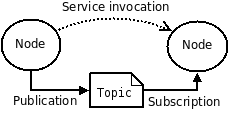
\includegraphics[scale=0.6]{image/appendixA_ROS_basic_concepts.png}
	\caption{\figlbl{ros_concept} source: \url{http://wiki.ros.org/ROS/Concepts}}
\end{figure}

\section{Before we start..}
Here are some useful Linux/ROS commands
\begin{itemize}
\item The command “ls” stands for (List Directory Contents), List the contents of the folder, be it file or folder, from which it runs.
\begin{lstlisting}[language=bash]
$ ls
\end{lstlisting}

\item The “mkdir” (Make directory) command create a new directory with name path. However is the directory already exists, it will return an
error message “cannot create folder, folder already exists”.
\begin{lstlisting}[language=bash]
$ mkdir <new_directory_name>
\end{lstlisting}

\item The command “pwd” (print working directory), prints the current working directory with full path name from terminal
\begin{lstlisting}[language=bash]
$ pwd
\end{lstlisting}

\item The frequently used “cd” command stands for change directory. 
\begin{lstlisting}[language=bash]
$ cd /home/user/Desktop
\end{lstlisting}
return to previous directory
\begin{lstlisting}[language=bash]
$ cd ..
\end{lstlisting}
Change to home directory
\begin{lstlisting}[language=bash]
$ cd ~
\end{lstlisting}

\item The hot key ``ctrl+c" in command line \textbf{terminates} current running executable.  If ``ctrl+c" does not work, closing your terminal as that will also end the running Python program. \textbf{DO NOT USE ``ctrl+z" as it can leave some unknown applications running in the background}.   

\item If you want to know the location of any specific ROS package/executable from in your system, you can use ``rospack" find  ``package name" command. For 
example, if you would like to find `lab2pkg\_py' package, you can type in your console
\begin{lstlisting}[language=bash]
$ rospack find lab2pkg_py
\end{lstlisting}

\item To move directly to the directory of a ROS package, use roscd. For example, go to lab2pkg\_py package directory
\begin{lstlisting}[language=bash]
$ roscd lab2pkg_py
\end{lstlisting}

\item Display Message data structure definitions with rosmsg
\begin{lstlisting}[language=bash]
# Display the fields in the msg
$ rosmsg show <message_type>
\end{lstlisting}

\item rostopic, A tool for displaying debug information about ROS topics,
including publishers, subscribers, publishing rate, and
messages.
\begin{lstlisting}[language=bash]
# Print messages to screen
$ rostopic echo /topic_name
# List all the topics available
$ rostopic list
# Publish data to topic
$ rostopic pub <topic-name> <topic-type> [data...]  
\end{lstlisting}
\end{itemize}

\section{Create your own workspace}
Since other groups will be working on your same computer, you should backup your code to a USB drive or cloud drive everytime you come to lab.  This way if 
your code is tampered with (probably by accident) you will have a backup.
\begin{itemize}
\item Log on to the computer as `rvc' with the password `123456'.  If you log on as `guest', you will not be able to use ROS.
\item First create a folder in the home directory, mkdir catkin\_(yourNETID).  It is not required to have "catkin" in the folder name but it is recommended.
\begin{lstlisting}[language=bash]
$ mkdir -p catkin_(yourID)/src
$ cd catkin_(yourID)/src
$ catkin_init_workspace
\end{lstlisting}
\item Even though the workspace is empty (there are no packages in the 'src' folder, just a single CMakeLists.txt link) you can still "build" the 
workspace. Just for practice, build the workspace.
\begin{lstlisting}[language=bash]
$ cd ~/catkin_(yourID)/
$ catkin_make
\end{lstlisting}
\item \textbf{VERY IMPORTANT}: Remember to \textbf{ALWAYS} source when you open a new command prompt, so you can utilize the full convenience of Tab completion in ROS.
Under workspace root directory:
\begin{lstlisting}[language=bash]
$ cd catkin_(yourID)
$ source devel/setup.bash
\end{lstlisting}
\end{itemize}

\section{Running a Node}
\begin{itemize}
\item Once you have your catkin folder initialized, add the UR3 driver and lab starter files.  The compressed file lab2andDanDriver.tar.gz, found
at the class website contains the driver code you will need for all the ECE 470 labs along with the starter code for LAB 2.  Future lab compressed 
files will only contain the new starter code for that lab.  Copy lab2andDriverPy.tar.gz to your catkin directories ``src" directory.  Change directory
to your ``src" folder and uncompress by typing ``tar -xvf lab2andDriver.tar.gz".  You can also do this via the GUI by double clicking on the compressed file and dragging the folders into the new location.

``cd .." back to your catkin\_(yourID) folder and build the code
with ``catkin\_make"
\item After compilation is complete, we can start running our own nodes. For example our lab2node node. However, before running any nodes, we must
have roscore running. This is taken care of by running a launch file.

\begin{lstlisting}[language=bash]
$ roslaunch ur_robot_driver ur3e_bringup.launch
\end{lstlisting}

This command runs both roscore and the UR3 driver that acts as a subscriber waiting for a command message that controls the UR3's motors.


\item Open a new command prompt with ``ctrl+shift+N", cd to your root workspace directory, and source it ``source devel/setup.bash".

\item We may also need to make lab2\_exec.py executable.
\begin{lstlisting}[language=bash]
$ chmod +x lab2_exec.py
\end{lstlisting}

\item Run your node with the command rosrun in the new command prompt. Example of running lab2node node in lab2pkg package: 
\begin{lstlisting}[language=bash]
$ rosrun ur3e_driver_ece470 ur3e_driver_ece470
# Another terminal
$ rosrun lab2pkg_py lab2_exec.py
\end{lstlisting}
\end{itemize}

% Note that the ``-{}-simulator True" tells it you are running on the simulator, while ``-{}-simulator False" tells the program you are running on real hardware.  This flag is currently only applicable to Lab 2.

\section{More Publisher and Subscriber Tutorial}
Please refer to the webpage: \url{http://wiki.ros.org/ROS/Tutorials/WritingPublisherSubscriber(c\%2B\%2B)}



% \chapter{V-rep Simulation}
\label{crashcourse}

The robotic control lab (3071 ECEB) receives a large volume of students with the expansion of ECE470 and ECE489. Lab space and work benches can be in high demand toward the end of the semester. Therefore, we highly encourage students to build and test your robot algorithms in simulation environments before deploying them on actual robots to relieve lab usage. Although any simulation software and environment that serve this purpose are welcomed, we recommend \textit{V-rep} for those of you who don't have any preference. \textit{V-rep} is a robot simulator with integrated development environment that is avaliable in Windows, Mac os, and Linux. Within \textit{V-rep}'s simulation environment, each object/model can be individually controlled via an embedded script, a ROS node, or a remote API client. And the script that is used to control robots in simulation can be written in C/C++, Python, Java, Lua, Matlab or Octave. These features make \textit{V-rep} adapt well to this course well and give students lots of freedom when conducting their own robot experiments without a physical robot. 

\section{Download and Install V-rep on your PC}
\begin{itemize}
\item Download the latest version of V-REP PRO EDU that suits your PC's operation system from: \url{http://www.coppeliarobotics.com/downloads.html}
\end{itemize}

\begin{figure}[h]
\centering
	
\includegraphics[scale=0.55]{appendixB_vrep_download.png}
\caption{\figlbl{downloadvrep}Download the latest version of V-REP PRO EDU}
\end{figure}

\begin{itemize}
\item For Windows users, launch and install the setup.exe file on your computer. It seems \textit{V-rep} prefers to be installed on C drive.
\item For Mac users, unzip the V-REP\_PRO\_EDU\_Vx\_x\_x\_Mac.zip folder and rename it if you prefer. Open a terminal inside the unzipped folder directory and type this command: 
\begin{lstlisting}[language=bash]
$ ./vrep.app/Contents/MacOS/vrep
\end{lstlisting}
\item For Linux users, unzip the V-REP\_PRO\_EDU\_Vx\_x\_x.tar folder and rename it if you prefer. Open a terminal inside the unzipped folder directory and type this command: 
\begin{lstlisting}[language=bash]
$ ./vrep.sh
\end{lstlisting}
\item To learn more about using \textit{V-rep} via command lines, visit:
\url{http://www.coppeliarobotics.com/helpFiles/en/commandLine.htm}
\end{itemize}

\section{Setup remote API to interface with V-rep}
\begin{itemize}
\item Follow instructions on \url{http://www.coppeliarobotics.com/helpFiles/en/remoteApiClientSide.htm} to enable the remote API with the programming language you prefer. (We recommend Python for ECE470)

\item You will be saving your remote API code in a different directory (any directory you want but preferably not the directory that contains \textit{V-rep}'s main program). For example, if you are using Python, create a new directory with a name you like, this new directory must contain the following files (besides the .tttt scene file and your Python remote API script) for the remote API function to work (See \figref{vrepwd}):

\textbf{vrep.py}

\textbf{vrepConst.py}

\textbf{remoteApi.dll, remoteApi.dylib or remoteApi.so} (depends on your operation system)

\end{itemize}

\begin{figure}[h]
\centering
	
\includegraphics[scale=0.7]{appendixB_vrep_folder.png}
\caption{\figlbl{vrepwd}An example of a working directory}
\end{figure}

\begin{itemize}
\item If you are a Python 3 user, we do have a remote API starter code for you to play with:
\url{http://coecsl.ece.illinois.edu/ece470/ece470_vrep_Linux.zip}
\url{http://coecsl.ece.illinois.edu/ece470/ece470_vrep_Win64.zip}
\end{itemize}

\section{Add a robot in your scene}
\begin{itemize}
\item Drag any robot of interest from the menu on the left hand side to the scene.

\end{itemize}
\begin{figure}[h]
\centering
	
\includegraphics[scale=0.2]{appendixB_vrep_robot.jpg}
\caption{\figlbl{vrepadd}Adding robot to your scene}
\end{figure}
\begin{itemize}

\item Re-position the robot using the move and rotate icons locate on the top menu bar.

\item Delete the default child script (\figref{vrepdelete}) from your robot before you try your remote API program, otherwise you will have two scripts that control the same robot.
\item Save the scene you created as .tttt file in the directory that contains your remote API script.
\end{itemize}

\begin{figure}[h]
\centering
	
\includegraphics[scale=0.3]{appendixB_Add_ur3.png}
\caption{\figlbl{vrepdelete}Delete the default child script from ur3}
\end{figure}


\section{Important notes!!}
\begin{itemize}
\item The dimension of the UR3 in \textit{V-rep} is somewhat different than the actual UR3 we use in lab. Therefore, when building your forward kinematics function in \textit{V-rep}, \textbf{DO NOT} use the dimensions from UR3's engineering drawing. Instead, you can use the following API function:
\begin{lstlisting}[language=bash]
vrep.simxGetObjectPosition()
\end{lstlisting}
to obtain the distance between two joint centers.

\item The drawback of using numerical solvers is the inconsistency between each simulation's result, especially in less significant digits (e.g. ans = 1.2345644 vs. ans = 1.234598). You may add a rounding step after some parameters of interest to reduce the chance of being inconsistent (e.g. round(ans) = 1.2346).

\item For detailed information on \textit{V-rep} API functions:

\underline{\textbf{Python}}

\url{http://www.coppeliarobotics.com/helpFiles/en/remoteApiFunctionsPython.htm}

\underline{\textbf{Matlab}}

\url{http://www.coppeliarobotics.com/helpFiles/en/remoteApiFunctionsMatlab.htm}

\underline{\textbf{C++}}

\url{http://www.coppeliarobotics.com/helpFiles/en/remoteApiFunctions.htm}

\end{itemize}
\chapter{Notes on Camera Calibration and Transformations}
\label{computervision}


\section{Simplified Perspective Transform}
To extract spatial information from camera images, we need to derive equations to compute an object's coordinates in the world frame $(x,y,z)_w$ 
based on row and column pixel coordinates in the image $(r,c)_c$.  Instead of giving you these equations, this section will walk through how the transform works to allow you to derive them yourself.

\begin{figure}[ht]
	\centering
		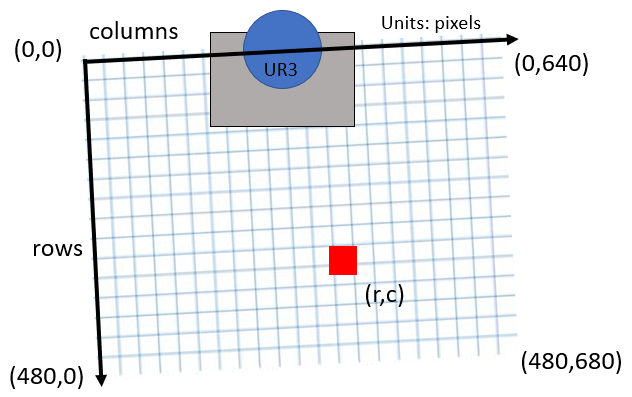
\includegraphics[height=6cm]{image/appendixC_camera_1.png}
	\caption{\figlbl{cam_1} The view from the camera.}
\end{figure}

The image starts as seen in \figref{cam_1}.  We can see that all data is in pixels, so the location of the object would be described by the rows and columns of the pixel at the centroid of the red block.  We can further see that the image is not square to the table, but instead slightly rotated.  We will ignore that for the time being.

\begin{figure}[ht]
	\centering
		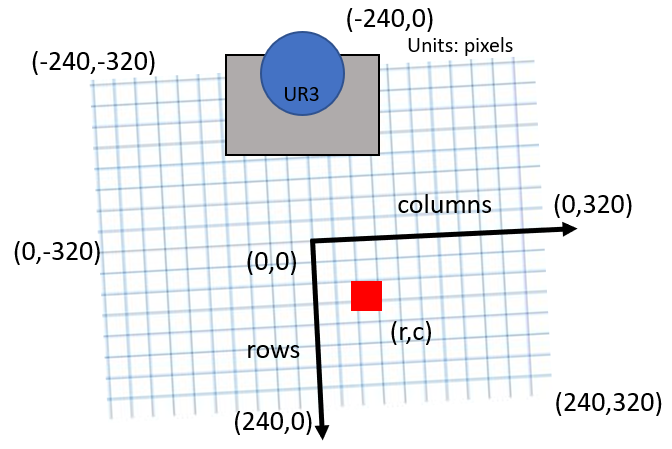
\includegraphics[height=6cm]{image/appendixC_camera_2.png}
	\caption{\figlbl{cam_2}  The view from the camera with the origin shifted to the principal point.}
\end{figure}
The first step is to translate the frame from the top left corner, to the center of the image also known as the principal point as seen in \figref{cam_2}.  As seen in Table \ref{tab:DOV}, the location of the principal point is in our original frame are called $\left(O_{r},O_{c}\right)$.  Based on this image, what are $O_{r}$ and $O_{c}$

\begin{eqnarray*}
	O_{r} & = & \\
	O_{c} & = &
\end{eqnarray*}
Side note: It is possible to develop the camera transformation without this translations, but shifting to the principle point is the standard method.  It is recommended that you consult a more exhaustive text on computer vision to better understand why.

The next step is to move from pixel measurements to something we can measure in the real world such as meters.  To do this, we need a relationship between pixel distance and physical distance on the table top. This value depends both on the physical properties of the camera and the distance between the camera and table top.  The physical properties of the camera are encapsulated by focal length ($f_{x}$ and $f_{y}$ as seen in Table \ref{tab:DOV}).  Because we do not know the focal length of the camera, we instead create a simple value $\beta$ which encapsulates both pieces of information:
\[
\beta=\frac{f_x}{z_c}=\frac{f_y}{z_c}. 
\]
This is a simplification of this relationship.  It assumes that pixels are square and that the lens does not distort the image at all.  Because of this, you might find it is less accurate at the edges of the image, but it should work fine for our purposes.  The units of $\beta$ are pixels per meter.

We now have enough information to complete our first equation.  This equation gives us the location of the block in meters, but with respect to the camera frame and not the world frame.  These equations are often called the \textbf{intrinsic} equations because they rely on the intrinsic properties of the camera such as $O_{r}$, $O_{c}$, $f_{x}$ and $f_{y}$ (i.e. properties that don't change).  These equations are essentially a transition from the camera sensor to the tabletop as seen in \figref{cam_3}.  Please complete the intrinsic equations using only $\beta$, $O_{r}$, and $O_{c}$
\begin{eqnarray*}
	x_c(r) & = & \\
	y_c(c) & = &
\end{eqnarray*}

\begin{figure}[ht]
	\centering
		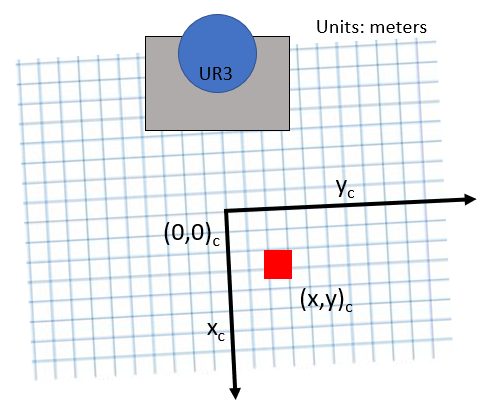
\includegraphics[height=6cm]{image/appendixC_camera_3.png}
	\caption{\figlbl{cam_3} The camera frame projected onto the table top.  This is the output of the intrinsic equations.}
\end{figure}


Now that we have the intrinsic equations and have transitioned to the table top, we can try to align this table top camera frame with the world frame at the corner of the aluminum plate.  We start this by shifting the frame from its current position which sits where the principal point lines up on the table top as shown in \figref{cam_4}.  As seen in Table \ref{tab:DOV}, the relationship between these two frames is $O_{cw}$ which is the origin of the world frame in terms of the camera frame.  The key values here are $T_{x}$ and $T_{y}$ as $T_{z}=0$.



\begin{figure}[ht]
	\centering
		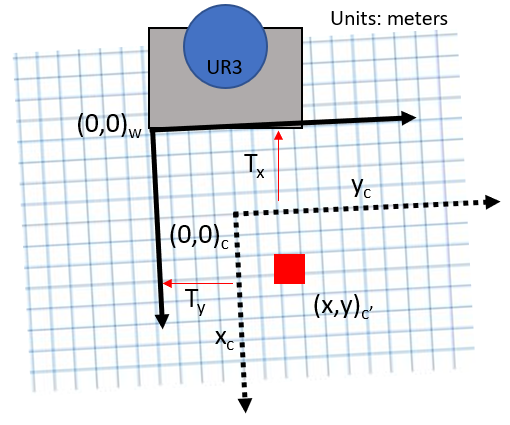
\includegraphics[height=6cm]{image/appendixC_camera_4.png}
	\caption{\figlbl{cam_4} The table top camera frame must be translated to align with the world frame.}
\end{figure}

Now that we have aligned the origins, it is time to straighten up the frame as shown in \figref{cam_5}.  We do this naturally by a rotation about the z-axis by the angle $\theta$.  We can see in Table \ref{tab:DOV} that $\theta$ is defined for $R_{cw}$.


\begin{figure}[ht]
	\centering
		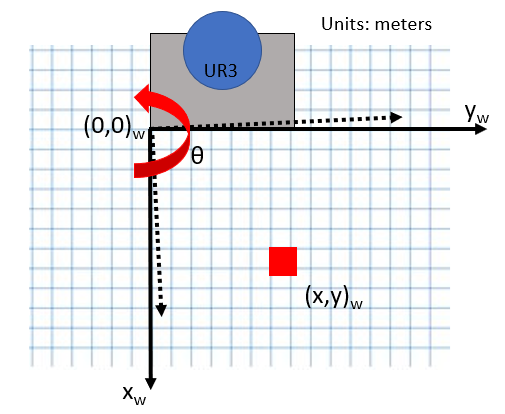
\includegraphics[height=6cm]{image/appendixC_camera_5.png}
	\caption{\figlbl{cam_5} The table top camera frame must be rotated to align with the world frame.}
\end{figure}


Now that we have translated and rotated our frame to align with the world frame, we can write the \textbf{extrinsic} equations.  These are known as extrinsic equations because they are based on values outside of the camera and change depending on placement and orientation.  Let's write the extrinsic equations:

\[
\left[\begin{array}{c}
x_w \\ y_w
\end{array}\right] = 
\]



Pay special attention to the signs of $T_{x}$ and $T_{y}$! 

We now have both the intrinsic and extrinsic equations and we can put them both together:

\begin{eqnarray*}
	x_w(r,c) & = & \\
	y_w(r,c) & = &
\end{eqnarray*}

These are the equations that you will use in your code to perform the camera transformation.  What about $z_w$?  Well, since we are working on the flat table top, $z_w$ is just the height of any object we wish to pick up.  A value for $z_w$ is provide in the code.

\begin{table}
	\centering
	\begin{tabular}{cl}
			Name & Description \\
		  \hline
			$(r,c)$     & (row,column) coordinates of image pixel \\
			$f_x,f_y$ & ratio of focal length to physical width and length of a pixel \\
			$(O_r,O_c)$ & (row,column) coordinates of {\it principal point} of image\\
            & (principal point of our image is center pixel) \\
			$(x_c,y_c)$ & (meters) coordinates of point in camera frame \\
% 			$p^c$	    & = $[x^c y^c z^c]^T$coordinates of point in camera frame \\
% 			$p^w$	    & = $[x^w y^w z^w]^T$coordinates of point in world frame \\
			$O_{cw}$		& = $[T_x T_y T_z]^T$ origin of world frame expressed in camera frame \\
			$R_{cw}$     & rotation expressing world frame w.r.t. camera frame. \\
		  \hline
	\end{tabular}
	\caption{Definitions of variables necessary for camera calibration.}
	\label{tab:DOV}
\end{table}


\section{Camera Calibration}
After formulating the camera transformation it is natural to ask how the key values such as $\beta$, $\theta$, $T_{x}$ and $T_{y}$ are found.  This is through the process of camera calibration.  Due to simulation limitations, this has already been done for this lab.  This section will give a brief introduction to how this process works.
\begin{itemize}
    \item $\beta$ - This value is found using a calibration stick.  The stick has two target set 10cm apart (center to center).  When the centroids of these targets are found, their distance in pixels can be determined.  It is then just a matter of relating the pixels to the fixed 10cm distance.
    \item $\theta$ - The same calibration stick is used again.  It is placed on the table top such that it carefully aligns with the y-axis of the world frame.  When the centroids of the targets are found, a right triangle can be formed with the two points and the angle formed will be $\theta$.
    \item $T_{x}$ and $T_{y}$ - This time a single target is placed on the table top with a known position in the world frame.  With this known positions, the location of the centroid (r,c) and $\beta$ and $\theta$, the only unknown in the camera transformation equations are $T_{x}$ and $T_{y}$, which can easily be solved for.
\end{itemize}







\chapter{VMware Installation and Simulator Guide}

\section{System Requirements}

\begin{itemize}
    \item CPU: i3 desktop or equivalent/ i5 laptop or equivalent
    \item GPU: Integrated Graphics Unit/ Dedicated GPU
    \item Memory: 6G or above
    \item Disk Space: 20G or above
\end{itemize}

Reference Laptop:
\begin{itemize}
    \item CPU: i5 8th Gen
    \item GPU: Intel UHD Graphics 620
    \item Memory: 8G
    \item Disk Space: 20G
\end{itemize}

Note: Simulators are demanding software to run. If you have problems running the virtual machine and/or the simulator, please let the TAs know about your situation. If you believe that it is due to hardware limitations, please check out the technology loan program \url{https://answers.uillinois.edu/illinois/99680}.

\newpage

\section{VMware Installation}

The UIUC WebStore offers free VMware products under VMware Academic Program. \url{https://e5.onthehub.com/WebStore/Welcome.aspx?ws=6c313875-25d6-e311-93fd-b8ca3a5db7a3}\\

Follow the instructions and download VMware Workstation 15.x Player on Windows/Linux or VMware Fusion 11.x Pro for Mac. Note that the guide is only written for VMware Workstation 15.x but not on VMware Fusion 11.x Pro. Please let the instructors know if you experience issues with Mac.

\section{VMware Image}

VMware uses VM image files to run the operating system as well as store files. Please unzip the ECE470VM.zip file and extract it to a working directory. In VMware, click “Open a Virtual Machine” and navigate to your working directory.

\begin{figure}[ht]
	\centering
		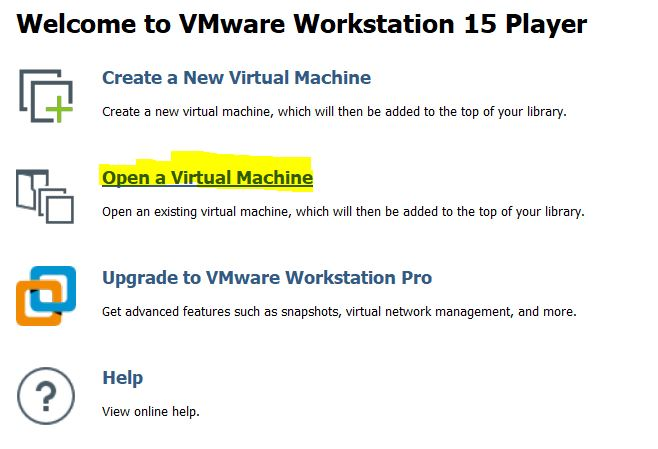
\includegraphics{image/appendixD_vm_open.JPG}
	\caption{Open a Virtual Machine}
\end{figure}

Double click the “ECE470VM.vmx” and you will see the “ECE470VM” option on the left side.

\begin{figure}[ht]
	\centering
		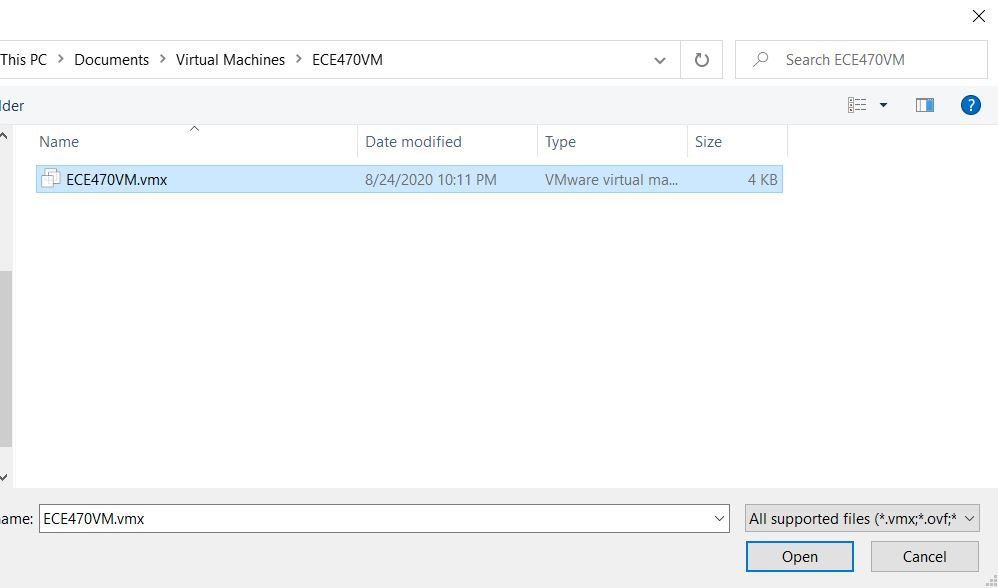
\includegraphics[scale=0.6]{image/appendixD_vm_open_2.JPG}
	\caption{Open vmx file}
\end{figure}

For memory, you need at least 4 GB to run the simulation. Because the host system also requires memory to run, the requirement for memory is at least 6 GB. If your computer has less than 6 GB memory, you need to contact the TAs and use the technology loan program.\\

Now you are ready to boot the system. Click “Play virtual machine” to boot the system. In the new box that asks about whether you moved or copied the virtual machine, choose "I Copied It".

\begin{figure}[ht]
	\centering
		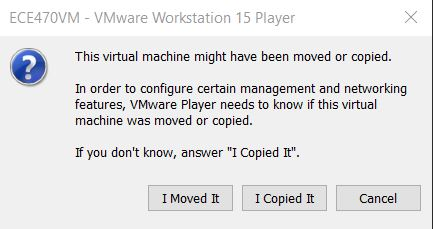
\includegraphics{image/appendixD_vm_copy.JPG}
	\caption{Click "I Copied It"}
\end{figure}

\section{Test}

In the lab, we are mainly going to use two software. To test their functionalities, open a terminal by the shortcut "Ctrl + Alt + T" or other way you prefer. In the terminal window, type in the following command:

\begin{lstlisting}[language=bash]
  $ roscore
\end{lstlisting}

The terminal should print out something similar to this:

\begin{figure}[ht]
	\centering
		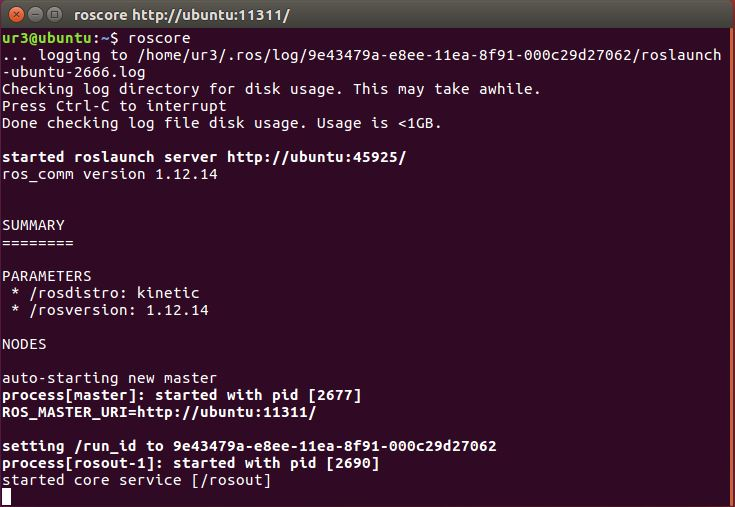
\includegraphics[scale=0.8]{image/appendixD_roscore.JPG}
	\caption{Result of Running "roscore"}
\end{figure}

Now you've tested basic functionalities of ROS, close the ROS core by "Ctrl + C". After the process ends, type in the following command:

\begin{lstlisting}[language=bash]
  $ gazebo
\end{lstlisting}

A new window should pop up and display something like this. If it somehow fails, try running it again. Let the TA know if Gazebo fails consistently. Similarly, after testing, close Gazebo by "Ctrl + C" in the terminal (not the new simulator window).

\begin{figure}[ht]
	\centering
		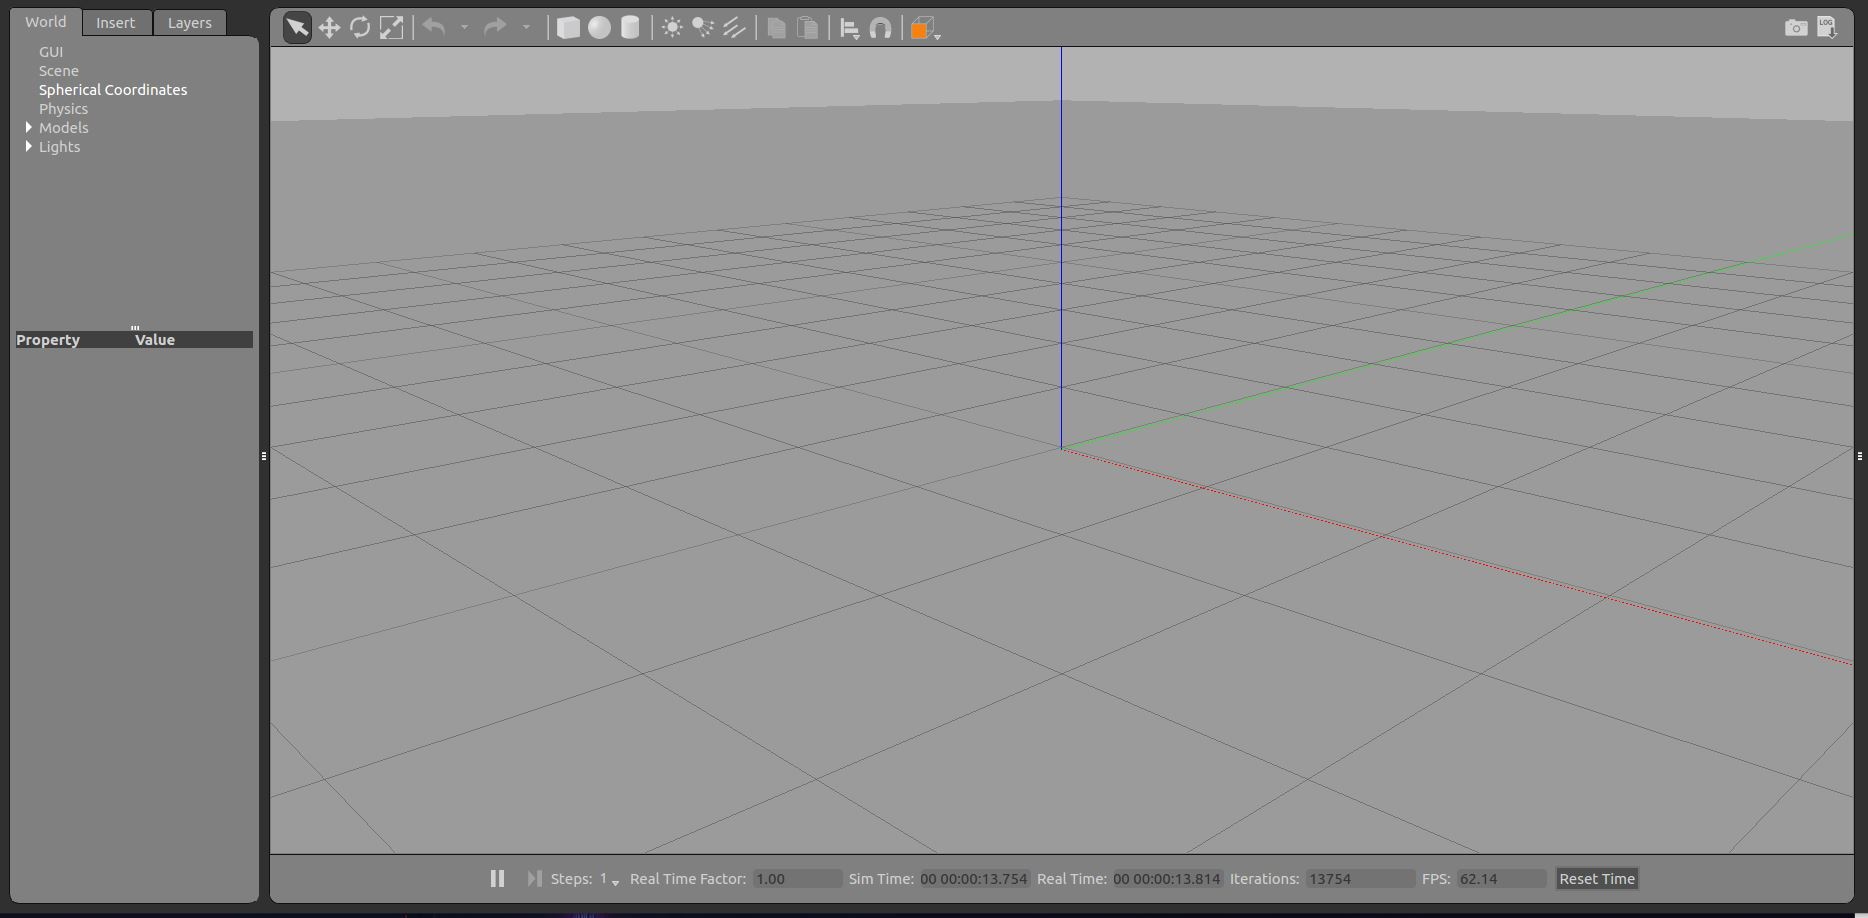
\includegraphics[scale=0.3]{image/appendixD_gazebo.JPG}
	\caption{Result of Running "gazebo"}
\end{figure}




\end{document}
